\documentclass[a4paper,12pt]{report}

\usepackage[cp1250]{inputenc}
%\usepackage[czech]{babel}

\usepackage{graphicx}
\usepackage{amsmath,amsthm}
\usepackage{amssymb}
\usepackage{amsfonts}
\usepackage{subfigure}
%\usepackage{subfloat}
\usepackage[usenames]{color}
%\usepackage[left=3.2cm,right=3.2cm,bottom=4.1cm,top=3.2cm]{geometry} 
\usepackage[left=3.5cm,right=2.5cm,bottom=4cm,top=3cm]{geometry} 
\usepackage{multirow}
\usepackage{enumerate}
\usepackage{epsfig}
\usepackage{accents}
\usepackage{verbatim}
\usepackage{easybmat}
\usepackage[titletoc]{appendix}
\usepackage{scrextend} %indenting
\usepackage{color}

\newlength{\dwidehatheight}
\newcommand{\doublewidehat}[1]{%
    \settoheight{\dwidehatheight}{\ensuremath{\widehat{#1}}}%
    \addtolength{\dwidehatheight}{-0.35ex}%
    \widehat{\vphantom{\rule{1pt}{\dwidehatheight}}%
    %\hat{\vphantom{\rule{1pt}{\dhatheight}}
    %\widehat{\hphantom{\rule{1pt}{5.5pt}{\dwidehatheight}}%
    \smash{\widehat{#1}}}}
    
\newcommand{\bm}[1]{\mbox{\boldmath{$#1$}}}
\newcommand{\sm}[1]{\mbox{\small{$#1$}}}
\newcommand{\ft}[1]{\mbox{\footnotesize{$#1$}}}
\newcommand{\ui}[1]{^{_{#1}}}
\newcommand{\li}[1]{_{^{#1}}}
\newcommand{\tr}{^{^{_\texttt T}}}
\newcommand{\diag}{\mathrm{diag}}
\setlength{\parindent}{10pt}
\numberwithin{equation}{chapter}

\newcommand{\assleq}{\, \mbox{$_{^{^\leq}}^{\hspace{-0mm}^{_{\textrm{as}}}\hspace{0.3mm}}$\ }}
\newcommand{\asleq}{\raisebox{0.5mm}{$\ _\leq$}\hspace{-2.4mm}\raisebox{1.7mm}{$^{_{_{_\textrm{as}}}}$}}
\newcommand{\asgeq}{\raisebox{0.5mm}{$\ _\geq$}\hspace{-2.4mm}\raisebox{1.7mm}{$^{_{_{_\textrm{as}}}}$}}
\newcommand{\aseq}{\ \mbox{$=^{\hspace{-2.7mm}^{_{\textrm{as}}}\hspace{0.3mm}}$\ }}
\newcommand{\aeeq}{\ \mbox{$=^{\hspace{-2.8mm}^{_{\textrm{ae}}}\hspace{0.3mm}}$\ }}
\newcommand{\aeaseq}{\ \mbox{$=^{\hspace{-2.7mm}^{_{\textrm{as}}}\hspace{0.3mm}} \raisebox{-2mm}{$\hspace{-4.5mm}^{_{\textrm{ae}}}\hspace{1.3mm}$}$\ }}

\newtheorem{thm}{Theorem}[chapter]
\newtheorem{lem}[thm]{Lemma}
\newtheorem{prop}[thm]{Proposition}
\newtheorem{cor}[thm]{Corollary}
\theoremstyle{definition}
\newtheorem{df}[thm]{Definition}

% Tato makra p�esv�d�uj� m�rn� o�kliv�m trikem LaTeX, aby hlavi�ky kapitol
% s�zel p���etn�ji a nevynech�val nad nimi spoustu m�sta. Sm�le ignorujte.
\makeatletter
\def\@makechapterhead#1{
  {\parindent \z@ \raggedright \normalfont
   \Huge\bfseries \thechapter. #1
   \par\nobreak
   \vskip 40\p@
}}
\def\@makeschapterhead#1{
  {\parindent \z@ \raggedright \normalfont
   \Huge\bfseries #1
   \par\nobreak
   \vskip 40\p@
}}
\makeatother

\title{}
\author{Pavol Stanek}

\begin{document}

%\thispagestyle{empty}
\begin{titlepage}
\begin{center}
\ \\

\vspace{15mm}

\large
Vrije Universiteit Amsterdam\\
Faculty of Sciences\\

\vspace{5mm}

{\Large\bf MASTER THESIS}

\vspace{10mm}

%%% Aby vlo�n� loga v�e spr�vn� fungovalo, je t�eba m�t soubor logo.eps nahran� v pracovn�m adres��i,
%%% tj. v adres��i, kde se nach�z� p�ekl�dan� zdrojov� soubor. Soubor logo.eps je mo�n� z�skat nap�.
%%% na adrese: http://www.mff.cuni.cz/fakulta/symboly/logo.eps

\includegraphics[scale =1] {LogoVU.jpg}
%{G:/School/MFF/Bakalarka/Bodove procesy/

\vspace{15mm}

%\normalsize
{\Large Pavol Stanek}\\ % dopl�te va�e jm�no
\vspace{5mm}
{\Large\bf Risk-Sensitive Control}\\ % dopl�te n�zev pr�ce
\vspace{5mm}
%Katedra pravd�podobnosti a matematick� statistiky\\ % dopl�te n�zev katedry �i �stavu
\end{center}
\vspace{30mm}

%\large
\noindent Supervisors: Mgr. Peter Dostal Ph.D., dr. Sandjai Bhulai 
\vspace{2mm}

\noindent Study programme: Stochastics and Financial Mathematics 

\vspace{\fill}
\begin{center}
2012
\end{center}

\end{titlepage} % zde kon�� �vodn� strana


\thispagestyle{empty}
\normalsize % nastaven� norm�ln� velikosti fontu
\setcounter{page}{2} % nastaven� ��slov�n� str�nek
\ \vspace{10mm} 

\noindent Before giving a formal start to this diploma thesis I would first like to thank Mgr. Peter Dostal Ph.D. and dr. Sandjai Bhulai for their careful supervision. %leading and valuable help with writing this thesis.

%R�d by som na tomto mieste po�akoval prof. RNDr. Viktorovi Bene�ovi, DrSc. za
%cenn� rady, �as a ochotu, ktor� mi venoval pri tvorbe tejto pr�ce. �alej by som r�d po�akoval Dr. D. Klementovi za poskytnutie d�t z neurofyziologick�ho experimentu. % dopl�te vlastn� text

\vspace{\fill} % nastavuje dynamick� um�st�n� n�sleduj�c�ho textu do spodn� ��sti str�nky
\noindent I hereby certify that I wrote this thesis on my own and that the references
include all the sources of information I have utilized. I agree with lending
this thesis.

\bigskip
\noindent Prague, June 18, 2012 \hspace{\fill}Pavol Stanek\\ % dopl�te pat�i�n� datum, jm�no a p��jmen�

%%%   V�tisk pak na tomto m�ste nezapome�te PODEPSAT!
%%%  
                                      
\tableofcontents % vkl�d� automaticky generovan� obsah dokumentu
\setcounter{page}{1}

\newpage % p�echod na novou str�nku
\addcontentsline{toc}{chapter}{\protect\numberline{}Abstract}
\chapter*{Abstract}
%%% N�sleduje strana s abstrakty. Dopl�te vlastn� �daje.

\noindent
Title: Risk-Sensitive Control\\
Author: Pavol Stanek\\
Department: Faculty of Sciences\\
Supervisor: Mgr. Peter Dostal Ph.D, dr.Sandjai Bhulai\\
%Supervisor's e-mail address: benesv@karlin.mff.cuni.cz\\

\noindent Abstract: This master thesis is concerned with risk-sensitive control of Markov decision chains. Risk sensitivity is represented by a exponential utility function. An iterative alghorithm for finding a control, that maximizes a long term growth rate of expexted utility is developed. The alghorithm is derived for both discrete time and continuous time chain. Results are applied on the problem of optimal management of portfolio with proportional transaction  costs. Dynamics of the value of a portfolio is derived and the consequent process is approximated by a Markov chain. Using the iterative alghorithm, the optimal trading strategy is numerically found.\\
%an optimal control is developed. By optimal is meant the one which maximizes the long term growth rate of expexted utility.
\\
\noindent Keywords: risk-sensitive control, Markov decision process, porfolio optimalization, proportional transaction cost
\newpage
\thispagestyle{empty}
\begin{titlepage}
\begin{center}
\ \\

\vspace{5mm}

\large
{\bf Univerzita Karlova v Praze}\\
\vspace{3mm}
{\bf Matematicko-fyzik�ln� fakulta}\\

\vspace{14mm}

{\Large\bf DIPLOMOV� PR�CE}

\vspace{10mm}

%%% Aby vlo�n� loga v�e spr�vn� fungovalo, je t�eba m�t soubor logo.eps nahran� v pracovn�m adres��i,
%%% tj. v adres��i, kde se nach�z� p�ekl�dan� zdrojov� soubor. Soubor logo.eps je mo�n� z�skat nap�.
%%% na adrese: http://www.mff.cuni.cz/fakulta/symboly/logo.eps

\includegraphics[scale =0.4] {Logo_MFF.jpg}
%\includegraphics[scale=0.3]{logo.eps}
%{G:/School/MFF/Bakalarka/Bodove procesy/

\vspace{15mm}

%\normalsize
{\Large Pavol Stanek}\\ % dopl�te va�e jm�no
\vspace{5mm}
{\Large\bf Exponenci�ln� ��zen� homogenn�ch markovsk�ch proces�}\\ % dopl�te n�zev pr�ce
\vspace{5mm}
Katedra pravd�podobnosti a matematick� statistiky\\ % dopl�te n�zev katedry �i �stavu
\end{center}
\begin{center}
\large
\begin{align*}
\noindent \text{Vedouc� diplomov� pr�ce: }& \text{Mgr. Peter Dost�l Ph.D.}\\ % dopl�te odpov�daj�c� 
\vspace{2mm} 
\noindent \text{Studijn� program: }& \text{Matematika}\\
\vspace{2mm} 
\noindent \text{Studijn� obor: }& \text{Pravd�podobnost, matematick� statistika }\\
                                & \text{a ekonometrie}% dopl�te odpov�daj�c� �daje
\end{align*}

\vspace{\fill}

Praha 2012
\end{center}

\end{titlepage} % zde kon�� �vodn� strana

\thispagestyle{empty}
\normalsize % nastaven� norm�ln� velikosti fontu
\setcounter{page}{2} % nastaven� ��slov�n� str�nek
\ \vspace{10mm} 

\noindent R�d by som na tomto mieste po�akoval Mgr. Peterovi Dost�lovi Ph.D za
cenn� rady, �as a ochotu, ktor� mi venoval pri tvorbe tejto pr�ce. %�alej by som r�d po�akoval Dr. D. Klementovi za poskytnutie d�t z neurofyziologick�ho experimentu.
 % dopl�te vlastn� text

\vspace{\fill} % nastavuje dynamick� um�st�n� n�sleduj�c�ho textu do spodn� ��sti str�nky
\noindent Prohla�uji, �e jsem tuto diplomovou pr�ci vypracoval samostatn� a v�hradn� s pou�it�m citovan�ch pramen�, literatury a dal��ch odborn�ch zdroj�.\\
\\
\noindent Beru na v�dom�, �e se na moji pr�ci vztahuj� pr�va a povinnosti vypl�vaj�c� ze z�kona �. 121/2000 Sb., autorsk�ho z�kona v platn�m zn�n�, zejm�na skute�nost, �e Univerzita Karlova v Praze m� pr�vo na uzav�en� licen�n� smlouvy o u�it� t�to pr�ce jako �koln�ho d�la podle � 60 odst. 1 autorsk�ho z�kona.\\
\\
\noindent V Praze dne 3.8.2012 \hspace{\fill}Pavol Stanek\\ % dopl�te pat�i�n� datum, jm�no a p��jmen�

%%%   V�tisk pak na tomto m�ste nezapome�te PODEPSAT!
%%%  
                                      
%\tableofcontents % vkl�d� automaticky generovan� obsah dokumentu
\setcounter{page}{1}

\newpage % p�echod na novou str�nku
\addcontentsline{toc}{chapter}{\protect\numberline{}Abstract}
%\chapter*{Abstract}
%%% N�sleduje strana s abstrakty. Dopl�te vlastn� �daje.
%\noindent
%N�zev pr�ce: Risk-Sensitive Control\\
%Autor: Pavol Stanek\\
%Katedra (�stav): Katedra pravd�podobnosti a metematick� statistiky\\
%Vedouc� bakal��sk� pr�ce: Mgr. Peter Dostal Ph.D.\\
%e-mail vedouc�ho: dostal@karlin.mff.cuni.cz\\

\noindent
N�zev pr�ce: Exponenci�ln� ��zen� homogenn�ch markovsk�ch proces�\\
Autor: Pavol Stanek\\
Katedra/�stav: Katedra pravd�podobnosti a matematick� statistiky MFF UK\\
Vedouc� diplomov� pr�ce: Mgr. Peter Dost�l Ph.D., Katedra pravd�podobnosti a matematick� statistiky MFF UK\\
%Supervisor's e-mail address: benesv@karlin.mff.cuni.cz\\
\\
\noindent Abstrakt: T�to diplomov� pr�ca sa zaober� exponenci�lnym riaden�m markovsk�ch re�azcov. V pr�ci je odvoden� itera�n� algoritmus na n�jdenie riadenia, ktor� maximalizuje mieru rastu o�ak�van�ho ��itku. ڞitok je meran� exponenci�lnou ��itkovou funkciou. Algoritmus je odvoden� pre re�azce v diskr�tnom aj spojitom �ase. V�sledn� algoritmus je n�sledne aplikovan� na probl�m optim�lneho riadenia portf�lia pri proporcion�lnych transak�n�ch n�kladoch. Je odvoden� dynamika v�voja investorovej poz�cie. V�sledn� proces je approximovan� markovsk�m re�azcom. Pou�it�m itera�n�ho algoritmu je numericky n�jden� optim�lna obchodn� strat�gia.\\
\\
\noindent Kl��ov� slova: exponenci�lne riadenie, markovsk� re�azec, optimaliz�cia porf�lia, proporcion�lne transak�n� n�klady

\vspace{\fill}

\noindent Title: Exponential control of homogeneous Markov processes\\
Author: Pavol Stanek\\
Department: Department of Probability and Mathematical Statistics, MFF UK\\
Supervisor: Mgr. Peter Dost�l Ph.D., Department of Probability and Mathematical Statistics, MFF UK\\
%Supervisor's e-mail address: benesv@karlin.mff.cuni.cz\\
\\
\noindent Abstract: This master thesis concerns exponential control of Markov decision chains.
An iterative alghorithm for finding a control, that maximizes a long term growth rate of expected utility is developed. The utility is measured by exponential utility function. The algorithm is derived for both discrete time and continuous time chain. Subsequently, the results are applied on the problem of optimally managing portfolio with proportional transaction  costs. The dynamics of the investor's position is derived and the consequent process is approximated by Markov chain. Using the iterative alghorithm, the optimal trading strategy is numerically found.\\
\\
\noindent Keywords: exponential control, Markov chain, portfolio optimization, proportional transaction costs
\newpage
\tableofcontents


%\tableofcontents
\addcontentsline{toc}{chapter}{\protect\numberline{}Introduction}
\chapter*{Introduction}
This master thesis concerns with optimal control of Markov decision chains%, where the optimality criterion incorporates risk sensitivity. 
We develop iterative alghorithm for finding optimal control and later we apply this algorithm to a portfolio management problem.

In first chapter we first introduce the concept of utility. We focus mainly on an exponential utility function which plays crucial role in our perfomance criterion. The peformance criterion is set as a long term growth rate of a certainty equivalent of the chain's payoff. The rest of the chapter is devoted to the derivation of an iterative alghorithm for finding an optimal control. The derivation is based on Perron-Frobenius theory concerning non-negative matrices. Resulting algorithm works similarly to the standard policy iteration procedure. We derive the algorithm for both discrete time and continuous time Markov decision chain.

In the second chapter we focus on the optimal portfolio allocation problem. We consider two assets. The first one represents a bank account and the other one represents some risky asset following a Geometric Brownian motion. Moreover proportional transaction costs are paid for trading the risky asset. We analytically derive the dynamics of the value of the portfolio consisting of these two assets. For the resulting process we construct approximation by both discrete time and continuous time Markov chain. Algorithms from the Chapter 1 is then used to numerically find  the strategy maximizing the long run performance criteria. Finally we compare results of both algorithms with analytical solution. %and we examine the dependence of the optimal strategy to the parameters of the model.% was examined. 

\chapter{Exponential Control of Markov Decision Chain}

In this chapter we are interested in Markov decision chains. Initial research in this field was done by Bellman \cite{Bellman}. He considered a Markov chain which pays a reward for moving from one state to another. Decision, affecting both transition probabilities and rewards, can by made in each state. Within this framework Howard \cite{Howard} derive iterative algorithm for finding a policy which maximizes a long time expected reward. Our aim in this chapter is to derive an algorithm similar to that of Howard, but under different optimality criteria. Our optimality criteria will incorporate risk-sensitivity. To be specific, we will maximize long time expected utility from reward represented by exponential utility function.

\vspace{4 mm}
%%%%%%%%%%%%%%%%%%%%%%%%%%%%%%%%%%%%%%%%%%%%%%%
\section{Exponential utility function}
\vspace{2 mm}

%\indent Let $S$ be an interval in $\mathbb{R}$. Denote all probability measures on $(S,\mathcal{B}(S))$ by $\mathcal{M}$. We interpret $\mathcal{M}$ as the set of all possible random pay-offs. %In this sense every $\mu\in\mathcal{M}$ can be considered as a {\em lottery}. 

In this section we introduce the concept of utility function. Especially we focus on the exponential utility function. We will show its basic properties and motivation for its usage. For more insight about utility, see the Chapter 2 in \cite{Portfolio}.

Imagine a lottery that pays certain prizes with certain probabilities. The outcome of the lottery is unknown, but what is known is its probability distribution. Interesting question is how much one should be willing to pay for opportunity to play such a lottery. Or, in other words, what is the fair price of a game. The first idea that crosses our mind is to take expected value as a fair price of a game. However according to this approach one is indifferent between lottery with a certain average pay-off and getting this amount of money straight away. In fact the majority of people would prefer the second alternative. %Thoughts similar to these led to the concept of utility. 
We see that the answer is not so simple. Certainly, it depends on players aversion to risk. Personal attitude to risk can be modeled by a utility function. %preferences over risky outcomes can be described by a utility function.
%Utility is described by a function which reflects personal preferences. answer not unique.
\begin{df} Let $S$ be an interval in $\mathbb{R}$. A function $u:S\to\mathbb{R}$ is called a \textit{utility function} if $u$ is strictly increasing, strictly concave and continuous on $S$.
\end{df}
\noindent Note that since concavity of a function on an open set implies its continuity, continuity requirement in the above definition concerns only boundary points of $S$.

Denote the set of all probability measures on $(S,\mathcal{B}(S))$ with finite expectation by $\mathcal{P}$. We interpret $\mathcal{P}$ as the set of all possible random pay-offs. In this sense every $\mu\in\mathcal{P}$ can be considered as a {\em lottery}. Denote the {\em expected utility} of the lottery $\mu$ by $U(\mu)$. That is
\[U(\mu)=\int_{\mathbb{R}} u\, d\mu.\]
The expected utility defines the preference relation $\succ$ on $\mathcal{P}$ by 
\[\mu\succ\nu\Leftrightarrow U(\mu)>U(\nu).\] 
The individual is willing to pay for the lottery with pay-off $\mu$ at most the amount of money $\texttt{CE}(\mu)$ which provides him the same utility. In other words, the individual is indifferent between lottery $\mu$ and a certain amount of money $\texttt{CE}(\mu)$. That means \[U(\mu)=U(\delta_{\texttt{CE}(\mu)})=u(\texttt{CE}(\mu))\]
 must be satisfied. The number $\texttt{CE}(\mu)$ is called {\em certainty equivalent}. Since $S$ is an interval, $U(\mu)\in S$ and due to monotonicity of $u$, we can write $\texttt{CE}(\mu)=u^{-1}(U(\mu))$. So the certainty equivalent is always defined and unique.

The requirement of strict concavity in the definition of utility function incorporates kind of risk averseness. Suppose the lottery $\nu$ that pays the amount $a$ with probability $p$ and the amount $b$ with probability $1-p$. If $a\neq b$, then by concavity 
\[p\,u(a)+(1-p)\,u(b)<u(p\,a+(1-p)\,b),\]
so $U(\nu)<u(\mathbb{E}(\nu))$. In words, receiving the amount of money equal to expected value of $\nu$ is preferred to playing the lottery $\nu$.

%A reasonable assumption on utility function is the {\em delta property}.
We say that a utility function fulfils the {\em delta property} if for $\Delta>0$ and $\mu\in\mathcal{P}$
\[\texttt{CE}(\mu + \Delta)=\texttt{CE}(\mu)+\Delta.\]
If the pay-off of a lottery is increased by the constant $\Delta>0$, certainty equivalent also increases by $\Delta$. It can be shown that the only utility function that possesses delta property is of the form
\begin{equation}
\label{expUF}
u(x)=a-b e^{-\gamma x}, \quad \gamma<0,
\end{equation}
where $b>0$ and $a\in\mathbb{R}$. A utility function of this type is called an {\em exponential utility function}. Since any increasing affine transformation of a utility function leads to the same preference relation on $\mathcal{P}$ and the same certainty equivalent, it is sufficient to consider exponential utility function with parameters $a=0$ and $b=1$.

If we relax the concavity condition in the definition of an utility function, then utility functions possessing delta property can be characterized as follows: It is either a linear function or a function of the type \eqref{expUF} with $\gamma\in\mathbb{R}$. Preferences described by a linear utility function coincides with the approach where the fair price of a lottery equals to its expected value.

The exponential utility function is also characterized by so called constant absolute risk aversion.
\begin{df}Suppose that a utility function $u$ is twice differentiable. Then the number
\[\alpha(x)=-\frac{u''(x)}{u'(x)}\]
is called the {\em Arrow-Pratt coefficient of absolute risk aversion} at the level $x$.
\end{df}
\noindent The exponential utility function is characterized by the property $\alpha(x)=-\gamma>0$. This can be easily shown by solving the respective differential equation. Due to this property the exponential utility function is often referred to as a constant absolute risk aversion (CARA) utility function.

The concept of expected utility can be naturally extended from lotteries to random variables with values in $S$. In the following sections we will examine the expected utility from a Markov reward chain under the exponential utility function.
\vspace{4 mm}
%%%%%%%%%%%%%%%%%%%%%%%%%%%%%%%%%%%%%%%%%%%%%%%%%%%%%%%%%%%%%%%%%%%%%%%%%%%%%%%%%%%%%%
\section{Exponential utility and Markov reward chain}
\vspace{2 mm}

Prior to the introduction of formal definition of a Markov chain, let us make a note on the definition that we will use. Throughout this thesis we will use a more general concept of Markov chain than can be found in introductory textbooks. We define a Markov chain not only by terms of probability distribution, but also by a filtration, which could be different from the one generated by the process. This approach is widely used in the general theory of Markov processes which considers continuous time and continuous state domain. See the monograph \cite{MP} for more insight. 

Fixing the filtration in the definition has such a consequence that we cannot consider different process when changing initial distribution. Instead the underlying probability measure changes and the process remains the same. With this approach we gain, beside a more general theory, a significant simplification of notation. So the computations will be more tractable. %Beside simplifying of the notation of conditional expectations we gain... in section... % of conditional expectations.

Let $\mathcal{X}$ be a finite set. Each $x\in\mathcal{X}$ is called a {\em state} and $\mathcal{X}$ is called the {\em state space}. Let $\bm{P}=\{p_{xy}\}_{x,y\in\mathcal{X}}$ be a stochastic matrix, that is a matrix with non-negative entries and with each row summing up to $1$. The matrix $\bm{P}$ is called the {\em transition matrix}. Denote entries of its $n$-th power by $p_{xy}^{(n)}$.

\begin{df} 
%Let $\bm{P}=\{p_{ij}\}_{i,j\in\mathcal{X}}$ be a stochastic matrix and $\bm{P}^n=\{p_{ij}^n\}_{i,j\in\mathcal{X}}$ be its $n$-th power. 
\label{DMCdef}
A system $(\Omega,\{\mathcal{F}_{n}\}_{n\in\mathbb{N}_0},X,\{\mathbb{P}_x\}_{x\in\mathcal{X}})$ is called a {\em (homogenous) Markov chain} with the transition matrix $\bm{P}$ if
\begin{enumerate}[(i)]
\item $\mathcal{F}_n$, $n\in\mathbb{N}_0$ are $\sigma$-fields on $\Omega$ satisfying $\mathcal{F}_m\subset \mathcal{F}_n$ for all $m\leq n$,
\item $X=\{X_n, n\in\mathbb{N}_0\}$ is $\mathcal{X}$-valued process defined on $\Omega$ and $X_m$ is $\mathcal{F}_n$ measurable for all $m\leq n$,
\item for all $x\in\mathcal{X}$, $\mathbb{P}_x$ is a probability measure on $\mathcal{F}_\infty=\sigma\left(\bigcup_{n=0}^{\infty}\mathcal{F}_n \right)$ satisfying for all $y\in\mathcal{X}$ and all $m,n \in \mathbb{N}_0$, $m\leq n$
$$\mathbb{P}_x(X_0=x)=1 \quad \text{and} \quad \mathbb{P}_x(X_n=y|\mathcal{F}_m)=p_{X_m,y}^{(n-m)}, \quad \mathbb{P}_x-a.s.$$ 
\end{enumerate}
%The set $\mathcal{X}$ is called a {\em state spate}. 
\end{df}
%Since $p^{(n-m)}_{X_m,j}$ is $\sigma\{X_m\}$-measurable, we have for any initial state $i\in\mathcal{S}$ 
%$$\mathbb{P}_i(X_n=j|\mathcal{F}_m)=\mathbb{P}_i(X_n=j|\sigma\{X_m\})\quad\mathbb{P}_i-a.s.$$
%So the additional information incorporated in the filtration $\mathcal{F}$ compering to the one generated by the process $X$ do not affect markovian property.

The property (iii) implies that the transition probability
\begin{equation}
\label{eqas}
\mathbb{P}_x(X_n=z|X_m=y) = p_{y,z}^{(n-m)} \quad \mathbb{P}_x-a.s. %=\mathbb{P}(X_n=z|X_m=y)
\end{equation}
almost surely does not depend  on the initial state $x$.
Consider a function $f$ defined on $\mathcal{X}$ and put%Conditional expectation of $f(X_n)$ can be expressed as
\[E^{(n)}_x f \triangleq \sum_{y\in\mathcal{X}} f(y)\,p^{(n)}_{x,y}=\bm{e}_x\tr\,\bm{P}^n\,f. \]
Then, using \eqref{eqas}, for all $x\in\mathcal{X}$ we have 
\[\mathbb{E}[f(X_n)|X_m=y]\aseq \sum_{z\in\mathcal{X}} f(z)\mathbb{P}_x(X_n=z|X_m=y)\aseq E_y^{(n-m)}f.\]
Consequently
\begin{equation}
\label{markov}
\mathbb{E}_x[f(X_n)|\mathcal{F}_m]=E_{X_m}^{(n-m)}\,f, \quad \mathbb{P}_x-a.s. \quad \text{for all } x\in\mathcal{X}.
%g_x(X_m)=g(X_m)
\end{equation}
We see that the conditional expectation $\mathbb{E}_x[f(X_n)|\mathcal{F}_m]$ is almost surely equal to the same random variable regardless of initial distribution. 
Thus we will write $\mathbb{E}$ instead of $\mathbb{E}_x$ in this case. Of course its distribution typically depends on the initial state, since change of the initial state means change of the underlying measure. The equation \eqref{markov} is often referred to as the Markov property.

Our definition treats explicitly only situation when the chain starts from arbitrary state $x$. However we can easily construct a probability measure that covers any initial distribution. Consider a probability distribution $\mu$ on $\mathcal{X}$. Define 
\begin{equation}
\label{PmuDef}
\mathbb{P}_{\mu}(A)=\sum_{x\in\mathcal{X}}\mu(x)\,\mathbb{P}_x(A)\quad A\in\mathcal{F}_{\infty}.
\end{equation}
Then $\mathbb{P}_{\mu}$ is a probability measure on $\mathcal{F}_{\infty}$ satisfying
\[ \mathbb{P}_x(X_n=y|\mathcal{F}_m) = \sum_{x\in\mathcal{X}} \mu(x)\,p^{(n-m)}_{X_m,y}=p^{(n-m)}_{X_m,y}, \quad \mathbb{P}_x-a.s.\]
So the Markov property holds for $\mathbb{P}_{\mu}$. Moreover \eqref{PmuDef} implies
\[ \mathbb{P}_{\mu}(X_0=x)=\sum_{y\in\mathcal{X}} \mu(y)\,\mathbb{P}_{y}(X_0=x)=\mu(x). \] 
In words, the chain has initial distribution $\mu$ under the measure $\mathbb{P}_{\mu}$.

As one expects the $n$-th power of $\bm{P}$ describes transition probabilities in $n$ periods. Indeed, for any states $x$ and $y$ we have
\[\mathbb{P}_x(X_n=y)=\mathbb{E}_x\mathbb{P}_x(X_n=y|\mathcal{F}_0)=\mathbb{E}_x\,p_{X_0,y}^{(n)}=p_{xy}^{(n)}, \quad \mathbb{P}_x-a.s.\]

We will restrict our consideration on Markov chains that have a agreeable behaviour described in a following couple of definitions.
\begin{df}
We say that a state $x$ is {\em accessible} from state $y$ if the $n$-step transition probability $p_{xy}^{(n)}$ is strictly positive for at least one $n$. A Markov chain is called {\em irreducible} if all states are accessible from each other.% if for all $i,j\in\mathcal{X}$ exists $n\in\mathbb{N}$ such that $p_{ij}^n>0$.
\end{df}
\begin{df}Let $x\in\mathcal{X}$ and let $d_x$ be the greatest common divisor of those $n\geq1$ for which $p_{x}^{(n)}$ is strictly positive. If $d_x>1$ then the state $x$ is called {\em periodic}. If $d_x=1$ then the state $x$ is called {\em aperiodic}. A Markov chain is called {\em aperiodic} if all states are aperiodic.
\end{df}
%More precisely, a fundamental result about Markov chains is that a finite state irreducible aperiodic chain has a unique stationary distribution p and, regardless of the initial state, the time-t distribution of the chain converges to p as t tends to infinity.

Now we add rewards to the chain. Suppose that the transition from state $x$ to state $y$ pays a reward $r(x,y)\in\mathbb{R}$ (sometimes denoted by $r_{xy}$). The matrix $\bm{R}=\{r_{xy}\}_{x,y\in\mathcal{X}}$ is called a {\em reward matrix} and a Markov chain enriched with a reward matrix is called {\em Markov reward chain}.

From now on we will consider an aperiodic irreducible Markov reward chain $X$ with the state space $\mathcal{X}=\{1,\dots,N\}$ and CARA utility function of the form
\begin{equation}
\label{euf}
\mathcal{U}_{\gamma}^{\texttt{C}}(x)=-e^{\gamma x}\quad\gamma<0.
\end{equation}
In Section 1.1 we explained that for fixed $\gamma$ exponential utility function of any form represents the same preference order. Therefore the specific choice \eqref{euf} does not impose any restriction on our consideration. The aim is to  compute the expected utility of the total reward of $X$ over the time and examine its asymptotic properties. For a given vector $\bm{b}\in\mathbb{R}^N$ define
\begin{equation}
\label{Udef}
U_n(\bm{b})\triangleq\mathcal{U}_{\gamma}^{\texttt{C}}\Big(\sum_{k=1}^n r(X_{k-1},X_k)\Big)\cdot\bm{b}(X_n).
\end{equation}
Here the symbol $\bm{b}(X_n)$ simply means the $X_n$-th component of the vector $\bm{b}$. Note that $U_n\triangleq U_n(\bm{1})$ is the total utility from reward over times $0,\dots,n$. Considering this quantity with arbitrary factor $\bm{b}(X_n)$ turns out to be useful. In order to avoid confusion, where it is desirable, we write the dot symbol indicating multiplication. Finally note that $U_n(\bm{b})$ can be equally expressed as
\begin{equation}
\label{WeirdNotation}
U_n(\bm{b})=U_n(\bm{1})\cdot\bm{b}(X_n)=U_n\cdot\bm{b}(X_n).
\end{equation}
First look at the conditional expectation of $U_n(\bm{b})$.
\begin{equation}
\label{ExpComutation}
\begin{split}
\mathbb{E}[U_n(\bm{b})|\mathcal{F}_{n-1}]&=\mathbb{E}\left[-\exp\left\{ \gamma\,\sum_{k=1}^{n-1} r(X_{k-1},X_k) \right\}\,\exp\{\gamma\,r(X_{n-1},X_n)\}\,\bm{b}(X_n)\Big|\mathcal{F}_{n-1}\right]\\
&=U_{n-1}\cdot\mathbb{E}[\exp\{\gamma\,r(X_{n-1},X_n)\}\,\bm{b}(X_n)|\mathcal{F}_{n-1}]\\
&\aseq U_{n-1}\cdot\sum_{i=1}^{N}\mathbb{I}_{[X_{n-1}=i]}\,\sum_{j=1}^{N}p_{ij}\,e^{\gamma\,r_{ij}}\,\bm{b}(j)
\end{split}
\end{equation}
Define the matrix $\bm{S}$ by
\begin{equation}
\label{S}
\bm{S}=\{s_{ij}\}_{i,j=1}^{N} \quad \text{with} \quad s_{ij}\triangleq p_{ij}\,e^{\gamma\,r_{ij}},
\end{equation}
Equally we can write the definition of $\bm{S}$ in matrix notation as
\begin{equation}
\label{Smform}
\bm{S}\triangleq\bm{P}\ast\bm{\exp}\{\gamma\,\bm{R}\}.
\end{equation}
where the symbol $\bm{\exp}$ represents exponential function applied entrywise and the symbol $\ast$ represents entrywise product, also known as Hadamard product. Contrary to the ordinary matrix multiplication, the Hadamard product is commutative. Now we can rewrite the second factor of the last term in \eqref{ExpComutation} as
\begin{equation}
\mathbb{E}[-\mathcal{U}_{\gamma}^{\texttt{C}}(r(X_{n-1},X_n))\,\bm{b}(X_n)|\mathcal{F}_{n-1}]=\bm{e}_{X_{n-1}}\tr\,\bm{S}\,\bm{b}=(\bm{S}\,\bm{b})(X_{n-1}),
\end{equation}
where $\bm{e}_k$ is the $k$-th canonical vector. Thus, using the notation \eqref{WeirdNotation}, we have 
\begin{equation}
\label{ConExp}
\mathbb{E}[U_n(\bm{b})|\mathcal{F}_{n-1}]=U_{n-1}\cdot(\bm{S}\,\bm{b})(X_{n-1})=U_{n-1}(\bm{S}\,\bm{b}).
\end{equation}
We make the following conclusion.
\begin{prop}
\label{prop1}
For any given vector $\bm{b}\in\mathbb{R}^N$, the variable $U_{n}(\bm{b})$ defined by \eqref{Udef} and $n\geq k\geq0$ we have 
$$\mathbb{E}[U_n(\bm{b})|\mathcal{F}_{n-k}]=U_{n-k}(\bm{S}^k\,\bm{b}),$$
where the matrix $\bm{S}$ is defined by \eqref{Smform}.
\end{prop}
\begin{proof}
Using induction the result immediately follows from \eqref{ConExp}.
\end{proof}
\noindent As a consequence we get the lemma which will be useful when we move to continuous time set-up. First generalize the definition \eqref{Udef} by putting
\begin{equation}
\label{UdefG}
U_{m,n}(\bm{b})\triangleq\mathcal{U}_{\gamma}^{\texttt{C}}\Big(\sum_{k=m+1}^n r(X_{k-1},X_k)\Big)\cdot\bm{b}(X_n)\in L_1,
\end{equation}
for $0\leq m<n$. Variable $U_{m,n}(\bm{b})$ is integrable because it attains only a finite number of values. Note that $U_{0,n}(\bm{b})=U_n(\bm{b})$ and 
\[U_{n}(\bm{b})=U_{n-k}\cdot(-U_{n-k,n}(\bm{b})).\] 
\begin{lem}
\label{LemmaSum}
For any given vector $\bm{b}\in\mathbb{R}^N$, the variable $U_{m,n}(\bm{b})$ defined by \eqref{UdefG} and $0<k<n$ we have
\[\mathbb{E}[-U_{n-k,n}(\bm{b})|\mathcal{F}_{n-k}]=(\bm{S}^k\,\bm{b})(X_{n-k}).\]
%$$\mathbb{E}\Bigg[-u\Big(\sum_{j=n-k+1}^n r(X_{k-1},X_k) \Big)\cdot\bm{b}(X_{n-k}) \Big|\mathcal{F}_{n-k} \Bigg]=(\bm{S}^k\,\bm{b})(X_{n-k}).$$
\end{lem}
\begin{proof}
Using Proposition \ref{prop1} and the fact that $U_{n-k,n}$ is integrable we get 
\[\mathbb{E}[U_n(\bm{b})|\mathcal{F}_{n-k}]=U_{n-k}\cdot\mathbb{E}[-U_{n-k,n}(\bm{b})|\mathcal{F}_{n-k}]=U_{n-k}\cdot (\bm{S}^k\,\bm{b})(X_{n-k}). \qedhere\]
\end{proof}
Now we can easily compute the expected utility of the reward up to time $n$.
\begin{cor} 
\label{cor1}
Denote $\bm{u}_n(\bm{b})=(u_{n,1}(\bm{b}),\dots,u_{n,N}(\bm{b}))\tr$, where $u_{n,i}(\bm{b})=\mathbb{E}_i[U_n(\bm{b})]$. Then
$$u_n(\bm{b})=-\bm{S}^n\bm{b}.$$
\end{cor}
\begin{proof}
Using Proposition \ref{prop1} with $n=k$ we get
\[\mathbb{E}_i[U_n(\bm{b})]=\mathbb{E}[U_n(\bm{b})|X_0=i]=U_0(\bm{S}^n\bm{b})=-(\bm{S}^n\bm{b})(i)=-\bm{e}_i\tr\bm{S}^n\bm{b}\quad \mathbb{P}_i - a.s.\qedhere\]
\end{proof}
Note that the $i$-th component of the vector $\bm{u}_n=\bm{u}_n(\bm{1})$ is equal to the total expected utility from reward over times $0,\dots,n$ when starting in state $i$ at time $0$. Corollary \ref{cor1} says that the time development of the total expected utility is described by the power of the matrix $\bm{S}$ defined by \eqref{S}.  %govern by it's largest eigenvalues 
Because the matrix $\bm{S}$ has non-negative entries we can apply Perron-Frobenius theory. This theory concerns the maximal eigenvalue of a non-negative matrix and consequently asymptotic properties of its power. For here used matrix results see Appendix A.

Because we assume that $X$ is irreducible and aperiodic, the matrix $\bm{P}$ is also irreducible and aperiodic (see Appendix A). The matrix $\bm{S}$ is constructed from $\bm{P}$ by multiplying each element by the positive number. Thus the matrix $\bm{S}$ also possesses mentioned properties. By the Perron-Frobenius theorem \ref{PF} the maximal eigenvalue of $\bm{S}$, that is the one with maximal Euclidean norm, is real and positive. Denote this eigenvalue by $\lambda>0$. Moreover the eigenvector $\bm{u}$ respective to eigenvalue $\lambda$ can be chosen, such that all its entries are positive, which we denote as $\bm{u}>0$. Further by Theorem \ref{PFlimit} we have
\begin{equation}
\label{limit}
\lim_{n\rightarrow\infty}\lambda^{-n}\,\bm{u}_{n}=\lim_{n\rightarrow\infty}-\lambda^{-n} \bm{S}^{n}\,\bm{1}=-k\,\bm{u},
\end{equation}
where $\bm{u}>0$ is an eigenvector respective to $\lambda$ and $k$ is a positive constant. Consequently for any initial state $i$
$$\lim_{n\rightarrow\infty}\frac{\bm{u}_{n+1}(i)}{\bm{u}_{n}(i)}=\lim_{n\rightarrow\infty}\lambda\,\frac{\lambda^{-(n+1)}\bm{u}_{n+1}(i)}{\lambda^{-n}\bm{u}_{n}(i)}=\lambda.$$
So for large times the utility is multiplied by $\lambda$ each time we move to the next state. This property holds regardless of initial state. That is the relation \eqref{limit} can be equivalently expressed as
\begin{equation}
\label{limprop}
\bm{u}_n=\lambda^n(k\,\bm{u}+o(\bm{1})) \quad n\rightarrow \infty.
\end{equation}
Now look what the preceding limiting property \eqref{limprop} means for the certainty equivalent. Denote the certainty equivalent of $U_n$ under CARA utility when starting in state $i$ by $\bm{\texttt{CE}}^{\texttt{C}}_{n}(i)$. That is  $\bm{\texttt{CE}}^{\texttt{C}}_n(i)$ is equal to $(\mathcal{U}_{\gamma}^{\texttt{C}})^{-1}(\bm{u}_n(i))$, where \[(\mathcal{U}_{\gamma}^{\texttt{C}})^{-1}(x)=\tfrac{1}{\gamma}\log(-x).\] 
Then we can express a limiting relation for certainty equivalent as follows
\begin{equation}
\label{cn}
\begin{split}
\bm{\texttt{CE}}^{\texttt{C}}_n&= \tfrac{1}{\gamma}\,\bm{\log}(-\bm{u}_n)\\
&= \tfrac{1}{\gamma}\,n\,\log\lambda\,\bm{1} +\tfrac{1}{\gamma}\,\bm{\log}(-k\,\bm{u}+o(\bm{1})), \quad n\rightarrow \infty,
\end{split}
\end{equation}
where $\bm{\log}$ represents logarithm function applied entrywise. Denote $\bm{z}\triangleq\tfrac{1}{\gamma}\bm{\log}(-k\bm{u})$ and 
\begin{equation}
\label{gdef}
g\triangleq\tfrac{1}{\gamma}\log\lambda.
\end{equation}
We can rewrite \eqref{cn} as
\begin{equation}
\bm{\texttt{CE}}^{\texttt{C}}_n = n\,g\,\bm{1} + \bm{z} +o(\bm{1}), \quad n\rightarrow \infty.
\end{equation}
The interpretation is that for large times the certainty equivalent increases by $g$ when the Markov chain moves to another state. The vector $\bm{z}$ is the correction reflecting the initial state. When time is large initial state becomes less important, which is expressed by the following limit holding for every initial state $i$
\begin{equation}
\label{CElimit}
\frac{\bm{\texttt{CE}}^{\texttt{C}}_{n}(i)}{n}\rightarrow g, \quad n\rightarrow\infty.
\end{equation}
In the next section we will look for optimal control of a Markov chain which maximizes certain equivalent growth rate $g$. Note that due to negativity of $\gamma$, \eqref{gdef} implies that maximization of $g$ is equivalent to the minimization of $\lambda$. This is a bit counter-intuitive and it is caused by the fact that our utility function attains only negative values. 
Finally note that the limit to be maximized, given by \eqref{CElimit}, can be equivalently expressed by previously used symbols as
\begin{equation}
\label{CritCh1}
%\lim_{n\rightarrow\infty} \tfrac{1}{n}\,u^{-1}(-U_n)
g=\lim_{n\rightarrow\infty}\tfrac{1}{\gamma}\,n^{-1}\,\log(-\mathbb{E}[U_n]).
\end{equation}
Before we proceed let us discuss an important special case. Sometimes the reward is not related with transition from one state to another but is paid when staying in a particular state. In this case the reward is described by a {\em reward vector} $\bm{r}=\{r_i\}_{i\in\mathcal{X}}$ determining a reward paid in each state. This is equivalent to considering the reward matrix $\bm{R}=\{r_{ij}\}_{i,j\in\mathcal{X}}$, with $r_{ij}=r_{i}$. Then the matrix $\bm{S}$ can be expressed as 
\begin{equation}
\label{QmformSpec}
\bm{S}=\bm{P}\ast\bm{\exp}\{\gamma\,\bm{R}\}=\bm{\exp}\{\gamma\,{\diag}(\bm{r})\}\cdot\bm{P}.
\end{equation}
\vspace{4 mm}
%%%%%%%%%%%%%%%%%%%%%%%%%%%%%%%%%%%%%%%%%%%%%%%%%%%%%%%%%%%%%%%%%%%%%%%%%%%%%%%%%%%%%%%%%%
\newpage
\section{Optimal risk sensitive control of Markov decision chain}
\vspace{2 mm}
We introduce the concept where a decision maker can effect the behaviour of the chain. In each state an action can be chosen. Vector of all actions selected in each state determines the rewards and the transition probabilities of the chain. %Lets move to formal definition.  
Formally consider a state space $\mathcal{X}$ and let $A_x$ be a finite set representing a set of all admissible actions in a state $x\in\mathcal{X}$. %The set \mathcal{A} is called {an action space}. 
%For all $x\in{\mathcal{X}}$ let $\mathcal{U}(x)\subset\mathcal{U}$ be a set of all admissible actions in a state $x$. 
Define an {\em action space} $\mathcal{A}$ as
\[\mathcal{A}=\prod_{x\in\mathcal{X}}A_x.\]
%$$\mathcal{A}=\{a:\mathcal{X}\rightarrow\mathcal{U} \text{, such that } a(x)\in\mathcal{U}(x)\}.$$
Further for any {\em policy} $a\in\mathcal{A}$ let $\bm{P}^{a}$ be a transition matrix  and let $\bm{R}^{a}$ be a reward matrix corresponding to this policy. That is for every policy $a\in\mathcal{A}$ we have a Markov reward chain $X^a$. The whole system $(\Omega,\{\mathcal{F}_n\}_{n\in\mathbb{N}_0},\{$X$^a\}_{a\in\mathcal{A}})$ is called {\em a Markov decision chain}.
%aperiodic irreducibile a Markov chain %A system $(\Omega,\{\mathcal{F}_n\}_{n\in\mathbb{N}_0},X,\{\mathbb{P}^{a}_x\}_{x\in\mathcal{X},a\in\mathcal{A}},\{R^{a}_x\}_{x\in\mathcal{X},a\in\mathcal{A}})$ is called {\em a Markov decision chain}. 
%Finally let $r:\mathcal{X}^2\times\mathcal{A}\rightarrow\mathbb{R}$ be a function determining reward for each policy. Such a system is called {\em a Markov decision chain}.
%$(\mathcal{X},\mathcal{U},\mathcal{A},\{\mathbb{P}(a)\}_{a\in\mathcal{A}},r)$ 

Consider a Markov decision chain with state space $\mathcal{X}=\{1,\dots,N\}$, transition matrices
\[\bm{P}^a=(\bm{p}_1(a_1),\dots,\bm{p}_N(a_N))\tr\] 
and reward matrices
\[\bm{R}^a=(\bm{r}_1(a_1),\dots,\bm{r}_N(a_N))\tr.\] 
We assume that for all policies $a\in\mathcal{A}$ the transition matrix $\bm{P}^a$ is aperiodic and irreducible. 
%Then for any fixed policy $a$, the process $X$ is a Markov reward chain with reward matrix $\bm{R}^a$ with entries $r^{a}_{i,j}=r(i,j,a)$, $i,j=1,\dots,N$. 
For any policy $a$ we have the variable $U_n^a(\cdot)$ defined like in \eqref{Udef} and the non-negative matrix $\bm{S}^{a}$ defined like in \eqref{Smform}. That is
\begin{align*}
\bm{S}^a=(\bm{s}_1(a_1),\dots,\bm{s}_N(a_N))\tr, \quad \bm{s}_i(a_i)&=\{s_{ij}(a_i)\}_{j=1}^{N},\\
 s_{ij}(a_i)&=p_{ij}(a_i)\,\exp\{\gamma \,r_{ij}(a_i)\}.
\end{align*}
By virtue of the Perron-Frobenius theorem \ref{PF} there exists the maximal eigenvalue $\lambda^a>0$ and respective eigenvector $\bm{v}^{a}>0$ of $\bm{S}^{a}$.
 
%For a given $\widehat{a}\in\mathcal{A}$ denote $\widehat{\lambda}=\lambda^{\widehat{a}}$ and $\widehat{\bm{v}}=\bm{v}^{\widehat{a}}$. 
 %$\bm{S}^a\,\bm{v}^{\widehat{a}}=\lambda^{\hat{a}}\,\bm{v}^{\hat{a}}$
\begin{equation}
\label{Mdef} 
M_{n}^{a}\triangleq(\lambda^a)^{-n}U_n^a(\bm{v}^a) \quad n\in\mathbb{N}_0,
\end{equation}
where the variable $U_n^{a}(\cdot)$ defined like in \eqref{Udef}.
\begin{prop}
\label{Mlem}
The process $M_{n}^{a}$ is a $\mathcal{F}_n$-supermartingale if $\bm{S}^a\bm{v}^a\geq\lambda^a\bm{v}^a$ entrywise. The process $M_{n}^{a}$ is a $\mathcal{F}_n$-martingale if $\bm{S}^a\bm{v}^a=\lambda^a\bm{v}^a$.
\end{prop}
\begin{proof}
As the Proposition concerns only one fixed policy, we will omit the upper index $a$ throughout the proof. Using Proposition \ref{prop1} and the fact that $M_{n-1}$ is $\mathcal{F}_{n-1}$ measurable we get
\begin{align*}
\mathbb{E}[M_n-M_{n-1}|\mathcal{F}_{n-1}]&\aseq(\lambda)^{-n}\,U_{n-1}(\bm{S}\bm{v}) - (\lambda)^{-n+1}\,U_{n-1}(\bm{v})\\
&=(\lambda)^{-n}[U_{n-1}(\bm{S}\bm{v})-\lambda\,U_{n-1}(\bm{v})]\\
&=(\lambda)^{-n}\,U_{n-1}\cdot[(\bm{S}\,\bm{v})(X_{n-1})-(\lambda\,\bm{v})(X_{n-1})].
\end{align*}
If $\bm{S}\,\bm{v}=\lambda\,\bm{v}$ the process $M_{n}$ is clearly an $\mathcal{F}_n$-martingal. Finally, from assumption $\bm{S}\,\bm{v}-\lambda\,\bm{v}\geq0$ and from facts that $\lambda$ is positive and $U_{n-1}$ is negative follows $\mathbb{E}[M_n|\mathcal{F}_{n-1}]\asleq M_{n-1}$. 
% and the result follows from the fact that $\widehat{\bm{v}}$ is positive. 
\end{proof}

\begin{thm}
\label{criteria2}
Let $\widehat{a}\in\mathcal{A}$. If the inequality $\bm{S}^a\bm{v}^{\widehat{a}}\geq\lambda^{\widehat{a}}\,\bm{v}^{\widehat{a}}$ holds for every policy $a\in\mathcal{A}$, than $\widehat{a}$ is an optimal policy in sense that $g^{\widehat{a}}\geq g^{a}$ for all $a\in\mathcal{A}$.
\end{thm}
\begin{proof}
%By the Lemma \ref{Mlem} 
For all $i$ we have
$$\frac{\sum_j s_{ij}(a_i)\,v^{\widehat{a}}_j}{v^{\widehat{a}}_i}\geq\lambda^{\widehat{a}}, \quad v^{\widehat{a}}_i>0.$$
Using the inequality from Theorem \ref{ineq} we get
$$\lambda^{a}\geq\min_i\frac{\sum_j s_{ij}(a_i)\,v^{\widehat{a}}_j}{v^{\widehat{a}}_i}\geq\lambda^{\widehat{a}}.$$
Remind that according to \eqref{gdef} the growth rate of certainty equivalent $g$ is equal to $\tfrac{1}{\gamma}\log\lambda$. Since $\gamma$ is negative we have $\widehat{g}\geq g^a$. %Consequently
\end{proof}
\begin{thm}[Policy iteration]
\label{PolicyIteration}
%Denote by $\bm{s}^a_i$ row vector corresponding to the $i$-th row of the matrix $\bm{S}^a$. 
Let $a_{0}\in\mathcal{A}$ be the initial policy. Define the sequence $\{a_n\}$ recursively by
\begin{equation}
\label{minimization}
a_{n+1}(i)\triangleq\underset{\alpha\in\mathcal{A}_i}{\operatorname{argmin}}\,\bm{s}_i(\alpha)\tr\,\bm{v}^{a_n}.
%a_{n+1}=\underset{a\in\mathcal{A}}{\operatorname{argmin}}\,\bm{S}^{a}\bm{v}^{a_n}
\end{equation}
If the minimum is attained for more the one policy and $a_n(i)$ is one of then, always make a conservative choice $a_{n+1}(i)=a_{n}(i)$. The resulting sequence $a_n$ converges to an optimal policy $\widehat{a}$.
\end{thm}
\begin{proof}
Suppose that $a_n$ converges to $\widehat{a}$. Then by \eqref{minimization} for all $i$ we have
\[\bm{e}_i\tr\,\bm{S}^a\,\bm{v}^{\widehat{a}}\geq \bm{e}_i\tr\,\bm{S}^{\widehat{a}}\,\bm{v}^{\widehat{a}}=\lambda^{\widehat{a}}\,v_i^{\widehat{a}}, \quad a\in\mathcal{A}.\]
Thus the inequality $\bm{S}^a\,\bm{v}^{\widehat{a}}\geq\lambda^{\widehat{a}}\,\bm{v}^{\widehat{a}}$ holds for every $a\in\mathcal{A}$ and the policy $\widehat{a}$ is optimal by virtue of Theorem \ref{criteria2}.

It now remains to show that $a_n$ converges. Because the action space is a discrete finite set, the sequence $a_n$ converges if and only if it is eventually constant. Thus it is sufficient to show that every time the procedure moves to a new policy it is better than the previous one. So suppose that $a_n \neq a_{n+1}$. Denote $a_n\triangleq a$ and $a_{n+1}\triangleq b$. Then by \eqref{minimization} the inequality 
%$\bm{s}^b_i\bm{v}^a\leq\lambda^a\bm{v}^a$ 
\[\bm{e}_i\tr\,\bm{S}^b\,\bm{v}^a=\bm{s}_i(b_i)\tr\,\bm{v}^a\overset{\eqref{minimization}}{\leq} \bm{s}_i(a_i)\tr\,\bm{v}^a=\bm{e}_i\tr\,\bm{S}^a\,\bm{v}^a=\lambda\,\bm{v}_i^a\]
holds for every $i$. In addition for some $i$ the inequality must be sharp, i.e.
\[\bm{S}^b\,\bm{v}^a \lneqq \lambda^a\,\bm{v}^a.\] 
Otherwise we would have $a=b$ due to the conservative choice. %$\bm{S}^b\bm{v}^a<\lambda^a\bm{v}^a$ holds.

Here we distinguish two cases. If $\bm{v}^a$ is an eingenvector of $\bm{S}^b$ respective to $\lambda^a$, then $\lambda^b\bm{v}^a<\lambda^a\bm{v}^a$. Because $\bm{v}^a$ has positive entries we have $\lambda^b<\lambda^a$ and consequently $g^b>g^a$.

Now suppose that $\bm{v}^a$ is not an eingenvector of $\bm{S}^b$ respective to $\lambda^a$. Then for all $i$
$$\frac{\sum_j s_{ij}(b_i)\,v_j^a}{v_i^a}\leq\lambda^a$$
with sharp inequality for some $i$. Using inequality from theorem \ref{ineq} we get
$$\lambda^b<\max_i\frac{\sum_j s_{ij}(b_i)\,v_j^a}{v_i^a}\leq\lambda^a$$
and consequently $g^b>g^a$. Note that the inequality is sharp, because $\bm{v}^a$ is not an eingenvector of $\bm{S}^b$.
\end{proof}

The Theorem \ref{PolicyIteration} gives us a method for finding the optimal policy. The algorithm can by summarized by the following steps: 
\begin{enumerate}
\item For every policy $a$ construct the matrix $\bm{S}^{a}$ according to \eqref{Smform}.
\item Choose an arbitrarily initial policy $a_n$, $n=0$.
\item Having the policy $a_n$, find an eigenvector $\bm{v}^{a_n}>0$ of the matrix $\bm{S}^{a_n}$ corresponding to its maximal eigenvalue.
\item Find the improved policy $a_{n+1}$ by entrywise minimization $\bm{S}^{a}\bm{v}^{a_n}$ over all policies $a$.
%\[a_{n+1}=\underset{a\in\mathcal{A}}{\operatorname{argmin}}\,\bm{S}^{a}\bm{v}^{a_n}\]
\item Repeat steps 3. and 4. until $a_n=a_{n+1}$. You have just find an optimal policy.
\end{enumerate}

\vspace{4 mm}
%%%%%%%%%%%%%%%%%%%%%%%%%%%%%%%%%%%%%%%%%%%%%%%%%%%%%%%%%%%%%%%%%%%%%%%%%%%%%%%%%%%%%%%%%%%%%%%%%%%%%%%
\section{Continuous time Markov reward chain}
\vspace{2 mm}
In order to define a continuous time Markov chain we start with a transition probabilities. Let $\mathcal{X}$ be a finite set and let $\{\bm{P}_t,t\geq 0\}$ with $\bm{P}_t=\{p_{xy}(t)\}_{x,y\in\mathcal{X}}$ be a system of stochastic matrixes satisfying
\begin{enumerate}[(B-1)]
\setlength\itemindent{15pt}
 \item $\bm{P}_0 =\bm{I}$,
 \item $\bm{P}_{s+t}=\bm{P}_s\,\bm{P}_t, \quad s,t\geq0$, 
 \item $\lim_{t\rightarrow0_+} \bm{P}_t = \bm{I}$.
\end{enumerate}
Property (B-2) is known as {\em Chapman-Kolmogorov relation}. Condition (B-1) together with (B-3)  assert that the system is right continuous at $t=0$. Moreover all three conditions together imply both sided continuity of the system $\{\bm{P}_t,t\geq 0\}$ in all $t\geq0$. Right continuity follows from computation
\begin{equation} 
\label{firstcourse1}
\lim_{h\rightarrow 0_+} \bm{P}(t+h)=\bm{P}(t)\lim_{h\rightarrow 0_+} \bm{P}(h)=\bm{P}(t)\bm{I}=\bm{P}(t). 
\end{equation}
On the other hand, for $t>h>0$ Chapman-Kolmogorov relation implies
\[\bm{P}_t=\bm{P}_{t-h}\bm{P}_h.\]
The matrix $\bm{P}_h$ is near to identity matrix for $h$ small enough and thus the inverse $\bm{P}_h^{-1}$ exists and also converges to identity matrix. So we have
\begin{equation} 
\label{firstcourse2}
\bm{P}_t=\bm{P}_t\,\lim_{h\rightarrow 0_+} \bm{P}_h^{-1}= \lim_{h\rightarrow 0_+} \bm{P}(t-h).
\end{equation}
Relations \eqref{firstcourse1} and  \eqref{firstcourse2} says that $\{\bm{P}_t,t\geq 0\}$ is continuous in all $t\geq0$ .

Remind that every matrix represents a linear operator and composition of linear operators corresponds to matrix multiplication.
Thus the above defined system together with matrix multiplication constitutes a continuous semigroup of linear operators on $\mathbb{R}^{|\mathcal{X}|}$.
\begin{df}
\label{CMCdef}
A system $(\Omega,\{\mathcal{F}_{t}\}_{t\in\mathbb{R}_0},X,\{\mathbb{P}_x\}_{x\in\mathcal{X}})$ is called a {\em (homogenous) continuous time Markov chain} with the transition probabilities $\{\bm{P}_t,t\geq 0\}$ if
\begin{enumerate}[(i)]
\item $\mathcal{F}_t$, $t \geq 0$ are $\sigma$-fields on $\Omega$ satisfying $\mathcal{F}_s\subset \mathcal{F}_t$ for all $s\leq t$,
\item $X=\{X_t, t\geq0 \}$ is $\mathcal{X}$-valued process on $\Omega$ and $X_s$ is $\mathcal{F}_t$ measurable for all $s\leq t$,
\item for all $x\in\mathcal{X}$ $\mathbb{P}_x$ is a probability measure on $\mathcal{F}_\infty=\sigma\left(\bigcup_{t\geq0}\mathcal{F}_t \right)$ satisfying for all $y\in\mathcal{X}$, $s,t \in \mathbb{R}_0$, $s\leq t$
$$\mathbb{P}_x(X_0=x)=1 \quad \text{and} \quad \mathbb{P}_x(X_t=y|\mathcal{F}_s)=p_{X_s,y}(t-s) \quad \mathbb{P}_x-a.s.$$ 
\end{enumerate}
%The set $\mathcal{X}$ is called a {\em state spate}.
\end{df} 
Similarly to the discussion after Definition \ref{DMCdef} we can show that the process possesses the Markov property and the matrix $\bm{P}(t)$ describes transition in time $t$ meaning that
\[p_{xy}(t)=\mathbb{P}_x(X_t=y).\] 
In discrete time the distribution of a Markov chain is fully described by initial distribution (in our case represented by underlying measure) and one step transition matrix. In continuous time there is no smallest transition step. In order to find similar simple description in continuous time we need to examine derivative of transition functions $p_{xy}(t)$, which is, loosely speaking, infinitesimal transition step. We have already seen that these functions are continuous, but it can be shown that they have much stronger properties. The key results are summarized in the following theorem.
%It can be shown thatFunctions $p_{xy}(t)$ are continuous
\begin{thm}
\label{Liget}
Let $\mathcal{X}$ be a countable set. Assume that the system $\bm{P}_t=\{p_{xy}(t)\}_{x,y\in\mathcal{X}}$ satisfies conditions (B-1)-(B-3) then
\begin{enumerate}[(i)]
\item For every $x,y\in\mathcal{X}$ the function $p_{xy}(t)$ is uniformly continuous in $t$. 
\item For all $x\in\mathcal{X}$ the derivative
\[q_x=-q_{xx}=-\frac{d}{dt_+}p_{xx}(t)\Big|_{t=0}\]
exists and $q_x\in[0,\infty].$ 
\item For all $x,y\in\mathcal{X}$, $y\neq x$ the derivative %If $q_x<\infty$ then for that $x$ and 
\[q_{xy}=\frac{d}{dt_+}p_{xy}(t)\Big|_{t=0}\]
exists and $q_{xy}\in[0,\infty)$.
\item If $q_x<\infty$ then $p_{xy}(t)$ is continuously differentiable in $t\geq 0$ for that $x$ and every $y\in\mathcal{X}$, and satisfies the Kolmogorov backward differential equation
\[\frac{d}{dt}p_{xy}(t)=\sum_{z\in\mathcal{X}} q_{xz} \, p_{zy}(t).\]
\end{enumerate}
\end{thm}
\begin{proof}
The proof can be found in \cite{Liggett}, theorems 2.13 and 2.14.
\end{proof}
%\begin{thm}
%Let $(\bm{P}_t, t\geq 0)$ be a system of transition matrices satisfying (a)-(c). Then for every state $x$ and $y$, $x\neq y$ following limits exist
%\[\lim_{h\rightarrow 0_+}\frac{1-p_{xx}(h)}{h}=q_x\in[0,\infty],\quad x\in\mathcal{X},\]
%\[ \lim_{h\rightarrow 0_+}\frac{p_{xy}(h)}{h}=q_{xy}\in[0,\infty),\quad x,y\in\mathcal{X}, x\neq y. \]
%\[\lim_{t\rightarrow 0_+}\frac{1-p_{xx}(t)}{t}=q_x,\quad\lim_{t\rightarrow 0_+}\frac{p_{xy}(t)}{t}=q_{xy}.\]
%Moreover $q_{xy}\in[0,\infty]$ and $q_x\in[0,\infty]$.
%\end{thm}
%\begin{proof}
%The proof can be found in \cite{Praskova} Chapter 14, Theorems 1.1 and 1.2.
%\end{proof}
The number $q_{xy}$ is called the {\em transition rates} from state $x$ to state $y$. The number $q_{x}$ is called the {\em total rate out of state} $x$. The larger the total rate is, the shorter time period the chain remains in state $x$. If $q_x=0$, the chain remains in $x$ permanently and we say that the state $x$ is {\em absorbing}. The state $x$ with $q_x<\infty$ is called {\em stable}. If $q_x=\infty$ the chain can not remain in $x$ for positive amount of time and we say that the state $x$ is {\em instantaneous}. However instantaneous states can occur only in case of infinite state space. In this thesis we work only with Markov chain with finite state space, so all states are stable. In this case
%If $q_{x}$ is finite have
\begin{equation}
\label{TotInt}
\sum_{y\neq x}q_{xy}=q_x.
\end{equation}
Indeed
\[0=\frac{1-\sum_y p_{xy}(t)}{t}=\frac{1-p_{xx}(t)-\sum_{y\neq x} p_{xy}(t)}{t}\longrightarrow q_x-\sum_{y\neq x}q_{xy}, \quad t\longrightarrow 0_+.\]
The relation \eqref{TotInt} justifies the name total rate. 
%Total rate has something to do with the amount time the chain stays in particular state. Suppose that the chain is in state $x$. Then the chain stays in $x$ for time $T_x=\inf{t>0:X_t\neq x}$ which has a exponential distribution with expected value equal to $1/q_i$.

Define the matrix $\bm{Q}$ by $\bm{Q}=\{q_{xy}\}_{x,y\in\mathcal{X}}$. Because all states are stable according to Theorem \ref{Liget} (iv) the {\em Kolmogorov backward differential equation} \eqref{KE} must hold.
\begin{equation}
\label{KE}
\frac{d}{dt}\bm{P}_t=\bm{Q}\,\bm{P}_t 
\end{equation}
From the properties of matrix exponential follows that under initial condition $\bm{P}_0=\bm{I}$ the equation \eqref{KE} has the unique solution of  the form
\begin{equation}
\label{InfGen}
\bm{P}_t=\exp\{t\,\bm{Q}\}.
\end{equation} 
So all transition probabilities can be expressed by means of the matrix $\bm{Q}$. In this sense $\bm{Q}$ is a continuous time counter-part of the one step probability matrix. The matrix \bm{Q} is called the {\em infinitesimal generator} or simply the {\em generator matrix}.

%The matrix $\bm{Q}=\{q_{xy}\}_{x,y\in\mathcal{X}}$ is called a {\em transition rate matrix}. 
%We will consider only Markov chains with finite rates. In this case the {\em intensity matrix}
%\[ \bm{Q}=\lim_{t\rightarrow0_+}\tfrac{1}{t}(\bm{P}_t-\bm{I}) \]
%is well defined and is of the form
%\[\bm{P}_t=\exp\{t\,\bm{Q}\}.\]

%Evidently the condition (c) implies that for all $x\in\mathbb{R}^{|\mathcal{X}|}$
%\[\lim_{t\rightarrow0_+}\left\| \bm{P}_t\,x-x \right\|=0,\]
%which together with conditions (a) and (b) indicates that the system $(\bm{P}_t , t\geq 0)$ creates a $C_0-$semigroup. It's {\em infinitesimal} generator is given by
%Define the {\em intensity matrix} $\bm{Q}=\{q_{xy}\}_{x,y\in\mathcal{X}}$ by
%\[ \bm{Q}=\lim_{t\rightarrow0_+}\tfrac{1}{t}(\bm{P}(t)-\bm{I}) \]
%It can be show that under assumptions (a)-(c) the limit exists. Numbers $q_{xy}$ $x\neq y$ are non-negative and finite and we call them {\em transition rates} from state $x$ to state $y$. Number $q_x=-q_{xx}$ are non-negative and can be also equal to $+\infty$ is total rate out of state $x$ 
%Out of main diagonal he Quantities out
%The matrix \bm{Q} is  called {\em an intensity matrix}.
%and the system of transition probabilities is of the form
%$$\bm{P}_t=\exp\{t\,\bm{Q}\}.$$


Now we add rewards to the process. Unlike in the case of a discrete time Markov chain, here the chain stays in every state generally different amount of time. Thus we need to evaluate separately staying in a particular state and transition from one state to another. Reward for staying in a particular state will be described by vector $\bm{r}$, where $r_i$ is a reward paid for being in state $i$ for one unit of time. Reward for a transition from one state to another will be described by matrix $\bm{R}$, meaning that moving from state $i$ to state $j$ pays a reward $r_{ij}$. Because the transition from state $i$ to state $i$ simply means staying in state $i$ and the corresponding reward is included in the vector $\bm{r}$, we assume that $r_{ii}=0$. A continuous time Markov chain with the vector $\bm{r}$ and the matrix $\bm{R}$ is called {\em a continuous time Markov reward chain}.

Consider a continuous time Markov reward chain $X$ with the state space $\mathcal{X}=\{1,\dots,N\}$. We try to do analogue of preceding sections in the continuous time set-up. For a given vector $\bm{b}\in\mathbb{R}^N$, similarly to \eqref{Udef} and \eqref{UdefG}, define
\begin{equation}
\label{UdefC}
U_{s,t}(\bm{b})=\mathcal{U}_{\gamma}^{\texttt{C}}\Big(\int_s^t r(X_v)\,dv+\sum_{s< v\leq t} r(X_{v-},X_{v}) \Big)\cdot \bm{b}(X_t)
\end{equation}
and put $U_{0,t}(\bm{b})=U_{t}(\bm{b})$. Note that the number of $v\leq t$, for which $X_{v-}\neq X_{v}$ is almost surely finite. Thus the sum on the right hand side is almost surely well defined. Again $U_t=U_t(\bm{1})$ is the total utility from the reward over the time interval $[0,t]$. The aim is to derive a formula for the conditional expectation of $U_t(\bm{b})$ similar to the one from Proposition \ref{prop1}.
\begin{equation}
\label{eqFactor}
\begin{split}
\mathbb{E}[U_t(\bm{b})|\mathcal{F}_s]&\aseq U_s\cdot \mathbb{E}\Big[-\mathcal{U}^{\texttt{C}}\Big(\int_s^t r(X_v)\,dv + \sum_{s< v\leq t} r(X_{v-},X_{v})\Big)\cdot \bm{b}(X_t)\Big|\mathcal{F}_s\Big]\\
&\aseq U_s\cdot \mathbb{E}[-U_{s,t}(\bm{b})|\mathcal{F}_s]
\end{split}
\end{equation} 
The idea is to approximate the continuous time Markov chain between $s$ and $t$ by the discrete time 
process obtained by observing the original one in discrete time instances. Such a process turns out be again a Markov chain and we can use Lemma \ref{LemmaSum} to express the second factor of the equation \eqref{eqFactor}. 

Denote  $\ft{t_{n,k}=s+\tfrac{k}{n}(t-s)}$ for $\sm{k=0,\dots,n}$ and consider the partition $\sm{\Delta_n=\{t_{n,k}\}_{k=0}^n}$ of the interval $\sm{[s,t]}$. Note that the norm of the partition $\Delta_n$ is equal to $\ft{\tfrac{t-s}{n}}$. Define the process
%$$ Y^{n}_k=X_{t_{n,k}}, \quad k=0,\dots, n. $$  
\[ X^{n}_v=X_{\lfloor v \rfloor_{\Delta_n}} \quad v\in[s,t],\]
%\[ X^{n}_v = X_{t_{n,k}} \quad v=[t_{n,k},t_{n,k+1}) \quad k=0,\dots, n. \]
where $\lfloor v \rfloor_{\Delta_n}$ means the value $v$ rounded down with respect to the set $\Delta_n$. The process $X^{n}$ has piecewise constant trajectories with jumps in points of partition $\Delta_n$.  Key properties of the constructed process are that the Markov property preserves and $X^{n}$ approximates well the original process $X$.
%The following lemma shows
\begin{lem}
\label{Skorochod}
\begin{enumerate}[(i)]
\item The process $\{X_{t_{n,k}}\}_{k=0}^n$ is a Markov chain with filtration %\newline $\{\mathcal{F}_{t_{n,k}},k=0,\dots,n\}$
$\{\mathcal{F}_{t_{n,k}}\}_{k=0}^n$ and the transition matrix $\bm{P}_{\frac{t-s}{n}}$.
\item Considering the processes $X^n=(X^{n}_v, v\in[s,t])$ and $X=(X_v,v\in[s,t])$ as random variables with values in the metric space $D[s,t]$ with Skorokhod metric,  $X^n$ converges to $X$ almost surely.
\end{enumerate}
\end{lem}
\begin{proof}
(i) 
All three required conditions from the Definition \ref{DMCdef} follow from their continuous-time couterparts from the Defintion \ref{CMCdef}. First two are obvious. The third one is shown by following computation. For any $\sm{0\leq k < l \leq n}$
\begin{equation}
\label{comput}
\begin{split}
\mathbb{P}(X_{t_{n,k}}=j|\mathcal{F}_{t_{n,l}})&=\mathbb{P}\left[X(s+\tfrac{k}{n}(t-s))=j|\mathcal{F}(s+\tfrac{l}{n}(t-s))\right]\\
&=p_{X_{t_{n,l}},j}(\tfrac{k-l}{n}t-s)  =\widetilde{p}_{X_{t_{n,l}},j}\ui{\,(k-l)},
\end{split}
\end{equation}
where $\widetilde{p}\li{i,j}\ui{\,(k-l)}$ is the entry of the \mbox{\small{$(k-l)$}}-th power of the matrix $\sm{\bm{P}_{\frac{t-s}{n}}}$ on $i$-th row and $j$-th column.
Note that the probability measures $\sm{\widetilde{\mathbb{P}}_{i}}$ can be defined by putting $\sm{\widetilde{\mathbb{P}}_{i}(X_{t_{n,0}}=i)=1}$. However the specific choice of measure does not influence the computation \eqref{comput}.% no matter how it is specified.

(ii) Remind that the Skorokhod metric is given by
\[ \rho(f,g)=\inf_{\lambda\in\Lambda}\Big( \left\|\lambda-I\right\| \vee \left\|f-g\circ\lambda\right\| \Big),\]
where $\left\|\cdot\right\|$ is the uniform norm on $[s,t]$ and $\Lambda$ is the set of all strictly increasing continuous bijection on $[s,t]$. We want to show that $\rho(X^n,X)$ almost surely goes to zero.

\begin{figure}[h]
\centering
\subfigure[Trajectories]{
   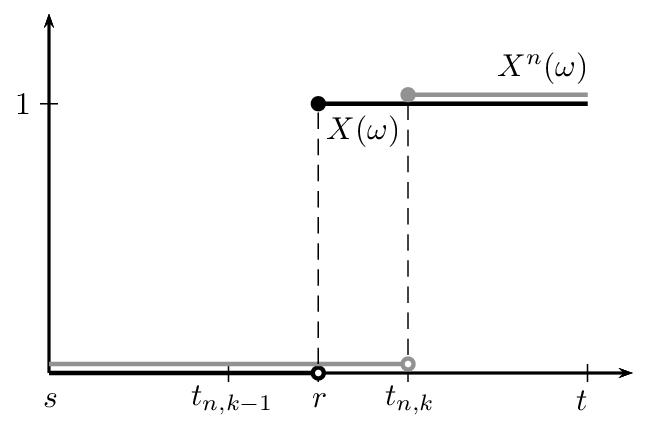
\includegraphics[scale =0.4] {obr1.jpg} %scale =0.4
   \label{skorochod1}
 }
 \subfigure[Time transformation]{
   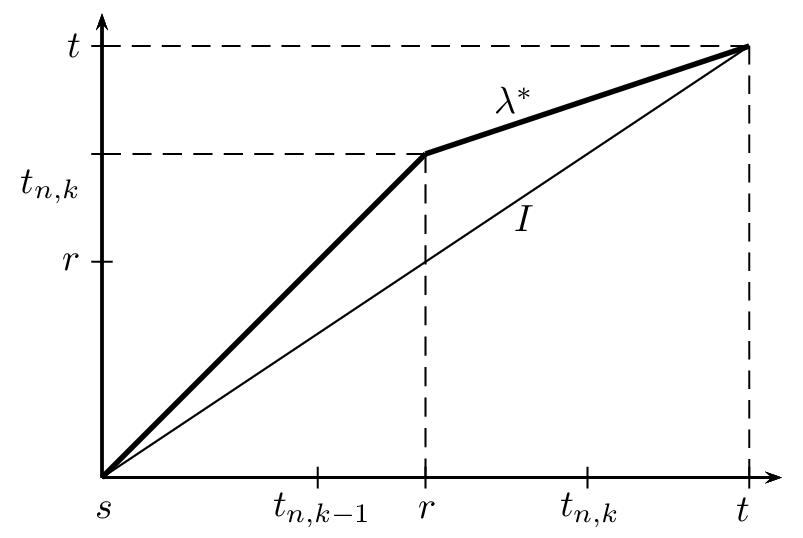
\includegraphics[scale =0.32] {obr2.jpg} %scale =0.32
   \label{skorochod2}
 }
\label{skorochod}
\caption{Reasoning for $X^n(\omega)\circ\lambda^*=X(\omega)$}
\end{figure}

For almost every  $\omega\in\Omega$ trajectory $X(\omega)$ has only finite number jumps in the interval $[s,t]$. Choose one such $\omega$. Because the state space is finite, size of each jump is finite. For clarity we will consider a trajectory $X(\omega)$ with only one jump of unit size. The general case with finite number of jumps is left as an exercise for the reader. So assume that $X(\omega)$ is of the form 
\[X(\omega,v)=\begin{cases}
0 & \text{if $v\in[s,r)$}\\ 
1 & \text{if $v\in[r,t]$}.
\end{cases}\]

For every partition $\Delta_n$ there exists $k$ for which $r\in(t_{n,k-1},t_{n,k}]$. 
As we can see from Figure \ref{skorochod1} the only difference between trajectories  $X^n(\omega)$ and $X(\omega)$ is that $X^n(\omega)$ is shifted right by $\sm{t_{n,k}-r}$. If we speed up the time appropriately on the interval $[0,r]$, the trajectory $X^n(\omega)$ would be equal to $X(\omega)$. Appropriate time transformation $\lambda^*\in\Lambda$ could be piecewise linear on intervals $[s,r]$, $[r,t]$ satisfying $\lambda^*(r)=t_{n,k}$. The function is plotted on Figure \ref{skorochod2}. Then evidently $X^n(\omega)\circ\lambda^*=X(\omega)$ and thus
\[\rho(X(\omega),X^n(\omega))\leq  \left\|\lambda^*-I\right\| \vee \left\|X(\omega)-X^n(\omega)\circ\lambda^*\right\| =\left\|\lambda^*-I\right\|\leq \left\|\Delta_n\right\|.\]
The result follows from the fact that the norm of the partition $\Delta_n$ goes to zero as $n$ goes to infinity.
\end{proof}
Like at the end of the previous section Section 1.2, define the matrix $\bm{\widetilde{R}}$ with entries $\widetilde{r}_{ij}=r_{i}$. When we replace the process $X$ by process the $X^n$ in equation \eqref{eqFactor}, we can express the second factor on the right hand side  as
\begin{equation}
\label{longterm}
\begin{split}
\mathbb{E}[-U_{s,t}^n(\bm{b})|\mathcal{F}_s]&\aseq\mathbb{E}\Big[-\mathcal{U}_{\gamma}^{\texttt{C}}\Big(\int_s^t r(X^n_v)\,dv + \sum_{s< v\leq t} r(X^n_{v-},X^n_{v})\Big)\cdot \bm{b}(X_t)\Big|\mathcal{F}_s\Big]\\
&\aseq\mathbb{E}\Big[-\mathcal{U}_{\gamma}^{\texttt{C}}\Big(\sum_{k=1}^n \tfrac{t-s}{n}\,r(X_{t_{n,k-1}})+\sum_{k=1}^n r(X_{t_{n,k}-},X_{t_{n,k}})  \Big)\cdot \bm{b}(X_t)\Big|\mathcal{F}_s\Big]\\
& \aseq \mathbb{E}\Big[ -\mathcal{U}_{\gamma}^{\texttt{C}}\Big(\sum_{k=1}^n \tfrac{t-s}{n} \widetilde{r}(X_{t_{n,k-1}},X_{t_{n,k}})+r(X_{t_{n,k-1}},X_{t_{n,k}})  \Big)\cdot \bm{b}(X_{t_{n,n}})\Big|\mathcal{F}_s\Big].
\end{split}
\end{equation}
Using Lemma \ref{LemmaSum} we can further simplify this term.
\begin{equation}
\label{longterm2}
\begin{split}
\mathbb{E}[-U_{s,t}^n(\bm{b})|\mathcal{F}_s]&\aseq \Big(\Big[\bm{P}_{\frac{t-s}{n}}\ast\bm{\exp}\{\gamma\,\tfrac{t-s}{n}\,\bm{\widetilde{R}}\} \ast\bm{\exp}\{\gamma\,\bm{R}\}\Big]^n\,\bm{b} \Big) (X_s)\\
&=\Big(\Big[\big(\exp\{\tfrac{t-s}{n}\,\gamma\,\diag(\bm{r})\}\cdot \exp\{\tfrac{t-s}{n}\,\bm{Q}\}\big) \ast\bm{\exp}\{\gamma\,\bm{R}\}\Big]^n\,\bm{b} \Big) (X_s).
%&=\Big(\Big[\exp\{\tfrac{t-s}{n}\,(\bm{Q}-\gamma\,\text{diag}(\bm{r}))\}\circ\bm{\exp}\{-\gamma\,\bm{R}\}\Big]^n\,\bm{b} \Big) (X_s)
\end{split}
\end{equation}
Using the Taylor expansion, it can be shown that last term converges to a finite limit. In spite of the simplicity of idea behind the proof, the proof itself is quite technical and tedious. Thus we move this computation to Appendix C. Now we can make the following conclusion.
%Accoring to the Proposition \ref{MatrixResult} the last term converges to a finite limit. 
\begin{prop}
\label{propC}
Let $0\leq s\leq s+h$. Then for any given vector $\bm{b}\in\mathbb{R}^N$ and the variable $U_{s+h}(\bm{b})$ defined by \eqref{UdefC} we have
$$\mathbb{E}[U_{s+h}(\bm{b})|\mathcal{F}_{s}]=U_{s}(\bm{S}^{h}\,\bm{b}),$$
where $\bm{S}^h$ has non-negative entries and is of the form
\begin{equation}
\label{SdefC}
\bm{S}^h=\exp\{h\,\bm{T}\}, \quad h\geq 0,
\end{equation}
where
\begin{equation}
\label{TdefC}
\bm{T}=(\bm{Q}+\gamma\,\diag(\bm{r}))\ast\bm{\exp}\{\gamma\,\bm{R}\}.
\end{equation}
\end{prop}
\begin{proof}
Define the functional $f$ on $D[s,t]$ by %\rightarrow\mathbb{R}
\[f(y)=-\mathcal{U}_{\gamma}^{\texttt{C}}\Big(\int_s^{s+h} r(y_v)\,dv + \sum_{s< v\leq s+h} r(y_{v-},y_{v})\Big)\cdot \bm{b}(y_t).\]
Because $f$ is continuous, according to Lemma \ref{Skorochod} $f(X^n)$ converges to the $f(X)$ almost surely. Moreover the sequence $f(X^n)$ is uniformly bounded, because the state space is finite. Thus we also have convergence in $L^1$ which implies convergence of conditional expectations. Now we can complete computation \eqref{longterm2} by taking the limit. The matrix $\bm{R}$ has zeros on its main diagonal. So according to the Lemma \ref{MatrixResult}
\begin{equation*}
\begin{split}
\lim_{n\rightarrow\infty}\Big[\exp\{\tfrac{h}{n}\,\gamma\,\diag&(\bm{r})\}\cdot \exp\{\tfrac{h}{n}\,\bm{Q}\} \ast\bm{\exp}\{\gamma\,\bm{R}\}\Big]^n\\
&=\exp\{(h)(\bm{Q}+\gamma\diag(\bm{r}))\ast\bm{\exp}\{\gamma\bm{R}\}\}=\bm{S}^{h}.\\
%&=\bm{S}^{t-s}
\end{split}
\end{equation*}
%Only non-negativity of $\bm{S}^h$ remains to be shown. This follows from the fact that 
The left hand side of the above term can be also expressed as %has non-negative entries because it can be expressed as... term  According to \eqref{longterm2} the matrix $\bm{S}^h$ can be also expressed as
$$\lim_{n\rightarrow\infty}\Big[\bm{P}_{\frac{h}{n}}\ast\bm{\exp}\{\gamma\,\tfrac{h}{n}\,\bm{\widetilde{R}}\} \ast\bm{\exp}\{\gamma\,\bm{R}\}\Big]^n.$$
So $\bm{S}^h$, $h\geq0$ is a limit of non-negative matrices and thus it is itself non-negative.
\end{proof}

%\begin{align*}
%\mathbb{E}\Big[&-u\Big(\sum_{k=1}^n \tfrac{t-s}{n}\,r(X_k^{s,t,n})+\sum_{k=1}^n r(X_{k-1}^{s,t,n},X_k^{s,t,n})  \Big)\cdot \bm{b}(X_t)\Big|\mathcal{F}_s\Big]\\
%& = \mathbb{E}\Big[ -u\Big(\sum_{k=1}^n \tfrac{t-s}{n} \widetilde{r}(X_{k-1}^{s,t,n},X_k^{s,t,n})+r(X_{k-1}^{s,t,n},X_k^{s,t,n})  \Big)\cdot \bm{b}(X^{s,t,n}_0)\Big|\mathcal{F}_s\Big]\\
%&= \Big(\Big[\bm{P}_{\frac{t-s}{n}}\circ\bm{\exp}\{-\gamma\,\tfrac{t-s}{n}\,\bm{\widetilde{R}}\} \circ\bm{\exp}\{-\gamma\,\bm{R}\}\Big]^n\,\bm{b} \Big) (X_s)\\
%&=\Big(\Big[\bm{P}_{\frac{t-s}{n}}\cdot\exp\{-\tfrac{t-s}{n}\,\gamma\,\text{diag}(\bm{r})\} \circ\bm{\exp}\{-\gamma\,\bm{R}\}\Big]^n\,\bm{b} \Big) (X_s)\\
%&=\Big(\Big[\exp\{\tfrac{t-s}{n}\,(\bm{Q}-\gamma\,\text{diag}(\bm{r}))\}\circ\bm{\exp}\{-\gamma\,\bm{R}\}\Big]^n\,\bm{b} \Big) (X_s).
%\end{align*}
%\begin{align}
%\Big[\bm{P}_{\frac{t-s}{n}}\circ\bm{\exp}\{-\gamma\,\bm{\widetilde{R}}\} \circ\bm{\exp}\{-\gamma\,\bm{R}\}\Big]^n&=\Big[\bm{P}_{\frac{t-s}{n}}\cdot\exp\{-\tfrac{t-s}{n}\,\gamma\,\text{diag}(\bm{r})\} \circ\bm{\exp}\{-\gamma\,\bm{R}\}\Big]^n\\
%&=\Big[\exp\{\tfrac{t-s}{n}\,(\bm{Q}-\gamma\,\text{diag}(\bm{r}))\}\circ\bm{\exp}\{-\gamma\,\bm{R}\}\Big]^n
%&=\exp\{(t-s)\,(\bm{Q}-\gamma\,\text{diag}(\bm{r}))\}\circ\bm{\exp}\{-\gamma\,\bm{R}\}
%\Big[\bm{P}_{\frac{t-s}{n}}\cdot\exp\{-\tfrac{t-s}{n}\,\gamma\,\text{diag}(\bm{r})\} \circ\bm{\exp}\{-\gamma\,\bm{R}\}\Big]^n%\exp\Big\{\tfrac{t-s}{n}\,\Big(\bm{Q}-\gamma\,\text{diag}(\bm{r})\Big)\Big\} \circ\bm{\exp}\{-\gamma\,\bm{R}\}\Big]^n
%&\longrightarrow \exp\Big\{(t-s)\,\Big(\bm{Q}-\gamma\,\text{diag}\{r_i\}_{i=1}^n\Big)\Big\} \circ\bm{\exp}\{-\gamma\,\bm{R}\}\Big\,\bm{b}(X_s)
%\end{align}
%It turns out that the last term converges to a finite limit. We can make the following conclusion.
%Denote $\bm{A}=\bm{Q}-\gamma\,\text{diag}(\bm{r})$ and $\bm{B}=\bm{\exp}\{-\gamma\,\bm{R}\}$. Than, because the matrix $\bm{R}$ has zeros on its main diagonal, $b_{ii}=1$ and according to Proposition \ref{MatrixResult} the last term converges to $\exp\{(t-s)\bm{A}\circ\bm{B}\}$. 
%\newpage
%$$r'(i,j)=\tfrac{t-s}{n}r(j)$$
%\begin{align}
%\mathbb{E}\Big[u\Big(\sum_{k=1}^n \tfrac{t-s}{n}\,r(X_k^{s,t,n}) \Big)\cdot b(X_t)\Big|\mathcal{F}_s\Big]&=
%[\bm{P}_{\frac{t-s}{n}}\circ\bm{\exp}\{-\gamma\,\bm{R}\}]^{n}\,b(X_s)\\
%&=\exp\Big\{\tfrac{t-s}{n}\,\bm{Q}\Big\}\,\exp\Big\{\tfrac{t-s}{n}\,\gamma\,\text{diag}\{r_1,\dots,r_N\}\Big\}\\
%&=\exp\Big\{\tfrac{t-s}{n}\,\Big(\bm{Q}-\gamma\,\text{diag}\{r_1,\dots,r_N\}\Big)\Big\}
%\end{align}
\vspace{2 mm}
%%%%%%%%%%%%%%%%%%%%%%%%%%%%%%%%%%%%%%%%%%%%%%%%%%%%%%%%%%%%%%%%%%%%%%%%%%%%%%%%%%%%%%%%%
\section{Optimal risk sensitive control of continuous time Markov decision chain}
\vspace{4 mm}

Similarly to the discrete time set-up, also here we add decisions to the process. Consider an action space
\[\mathcal{A}=\prod_{x\in\mathcal{X}}A_x,\]
 with $A_x$ representing the set of all admissible action in state $x$. For any policy $a\in\mathcal{A}$ let $\bm{Q}^a$ be an intensity matrix and $\bm{R}^a, \bm{r}^a$ be a reward matrix and a reward vector corresponding to the policy $a$. That is for every policy $a\in\mathcal{A}$ we have a continuous time Markov reward chain $X^a$.
 The whole system $(\Omega,\{\mathcal{F}_n\}_{n\in\mathbb{N}_0},\{$X$^a\}_{a\in\mathcal{A}})$ is called {\em a continuous time Markov decision chain}.

Consider a Markov decision chain with state space $\mathcal{X}=\{1,\dots,N\}$, intensity matrices
\[\bm{Q}^a=(\bm{q}_1(a_1),\dots,\bm{q}_N(a_N))\tr,\] 
reward matrices and reward vectors
\[\bm{R}^a=(\bm{r}_1(a_1),\dots,\bm{r}_N(a_N))\tr,\quad \bm{r}^a=(r_1(a_1),\dots,r_N(a_N))\tr.\] 
We assume that for all policies $a\in\mathcal{A}$ the chain is aperiodic and irreducibile. 
For any policy $a$ we have the variable $U_n^a(\cdot)$ defined by \eqref{UdefC} and the non-negative matrix  $\bm{S}^{a}=\exp\{\bm{T}^a\}$ defined by \eqref{SdefC} and \eqref{TdefC}. That is
\begin{align*}
\bm{T}^a=(\bm{t}_1(a_1),\dots,\bm{t}_N(a_N))\tr, \quad \bm{t}_i(a_i)&=\{t_{ij}(a_i)\}_{j=1}^{N},\\
 t_{ij}(a_i)&=(q_{ij}(a_i)+\gamma\,\delta_{ij}\,r_i(a_i)) \,e^{\gamma r_{ij}(a_i)},
\end{align*}
where $\delta_{ij}$ is the Kronecker delta. By virtue of the Perron-Frobenius theorem \ref{PF} the matrix $\bm{S}^a$ has its maximal eigenvalue $\lambda^a>0$ and respective eigenvector $\bm{v}^{a}>0$. In addition, according to the results of Appendix B, $\bm{v}^{a}$ is also an eigenvector of $\bm{T}^a$ coressponding to its maximal eigenvalue $\kappa^a\triangleq\log\lambda^a$.
%Consider a continuous time Markov decision chain with state space $\mathcal{X}=\{1,\dots,N\}$ such that for all policies $a\in\mathcal{A}$ the chain is aperiodic and irreducibile. For any fixed policy $a$ we have the nonnegative matrix $\bm{S}^a=\exp\{\bm{T}^a\}$ defined by \eqref{SdefC} and the variable $U_{t}^a(\cdot)$ defined by \eqref{UdefC}. 

%For a given $\widehat{a}\in\mathcal{A}$ denote $\widehat{\lambda}=\lambda^{\widehat{a}}$ and $\widehat{\bm{v}}=\bm{v}^{\widehat{a}}$. 
%$\exp\{u\widetilde{\bm{T}}\}=e^{-u\,\kappa}\,\bm{S}^{u}$
For fixed any $a\in\mathcal{A}$ consider a process
\begin{equation}
%\label{Mdef} 
M_{t}^{a}=(\lambda^a)^{-t}U_t^a(\bm{v}^a) \quad t\geq0.
\end{equation}
\begin{prop}
\label{MMlem}
The process $M_{t}^{a}$ is a $\mathcal{F}_t$-supermartingale if $\bm{T}^a\,\bm{v}^a\geq\kappa^a\,\bm{v}^a$. The process $M_{t}^{a}$ is a $\mathcal{F}_t$-martingale if $\bm{T}^a\,\bm{v}^a=\kappa^a\,\bm{v}^a$.
\end{prop}
\begin{proof}
As the Proposition concerns only one fixed policy, we will omit the upper index $a$ throughout the proof. %Denote $\kappa\triangleq\log\lambda$. 
First we want to show that the assumption $\bm{T}\,\bm{v}=\kappa\,\bm{v}$ implies the inequality  \[\exp\{s\,\bm{T}\}\,\bm{v}=\bm{S}^s\,\bm{v}\geq\lambda^s\,\bm{v}=e^{s\,\kappa}\,\bm{v} \quad\text{for all } s\geq0.\]
Using the fact $\exp\{-s\kappa\,\bm{I}\}=e^{-sk}\bm\,\bm{I}$ we compute
\begin{align*}
\bm{S}^s\,\bm{v}-\lambda^s\,\bm{v}&=\exp\{s\,\bm{T}\}\,\bm{v}-e^{s\,\kappa}\,\bm{v}\\
&=e^{s\,\kappa}\,(e^{-s\,\kappa}\,\exp\{s\,\bm{T}\}\,\bm{v}-\bm{v})\\
&=e^{s\,\kappa}\,(\exp\{s(\underbrace{\bm{T}-\kappa\,\bm{I}}_{\triangleq\widetilde{T}})\}-\bm{I})\,\bm{v}.
\end{align*}
The last equality is true due to the fact that matrices $\bm{T}$ and $\kappa\,\bm{I}$ commute. Denote $\widetilde{\bm{T}}\triangleq \bm{T}-\kappa\,\bm{I}$. Then by assumption $\widetilde{\bm{T}}\,\bm{v}\geq0$. We continue with computation as follows
\begin{align*}
\bm{S}^s\,\bm{v}-\lambda^s\,\bm{v}&=e^{s\,\kappa}\,(\exp\{s\widetilde{\bm{T}}\}-\bm{I})\,\bm{v}\\
&=e^{s\,\kappa}\,\left(\int_0^s \frac{\mathrm{d}}{\mathrm{d}u}\exp\{u\widetilde{\bm{T}}\}\mathrm{d} u \right)\,\bm{v}
=\underbrace{e^{s\,\kappa}}_{\geq 0}\,\left(\int_0^s \exp\{u\widetilde{\bm{T}}\}\mathrm{d} u\right) \,\underbrace{(\widetilde{\bm{T}}\bm{v})}_{\geq 0}.
\end{align*}
The integrant $\exp\{u\widetilde{\bm{T}}\}=e^{-u\,\kappa}\,\bm{S}^{u}$ is also non-negative according to Proposition \ref{propC}. Thus the whole term is nonnegative. 

We have shown that $\bm{S}^s\,\bm{v}\geq\lambda^s\,\bm{v}$, $s\geq0$. Employing  the Proposition \ref{propC} and the fact that $M_{s}$ is $\mathcal{F}_{s}$ measurable we get
\begin{align*}
\mathbb{E}[M_{s+h}-M_{s}|\mathcal{F}_{s}]&=\lambda^{-(s+h)}\,U_{s}(\bm{S}^h \bm{v}) - \lambda^{-s}\,U_{s}(\bm{v})\\
&=\lambda^{-s-h}[U_{s}(\bm{S}^h\bm{v})-\lambda^h\,U_{s}(\bm{v})]\\
&=\underbrace{\lambda^{-s-h}}_{> 0}\,\underbrace{U_{s}}_{< 0}\cdot[(\bm{S}^h\,\bm{v})(X_{s})-(\lambda^s\,\bm{v})(X_{s})].
\end{align*}
Because $\lambda$ is positive and $U_{s}$ is negative we have 
\[ \lambda^s\,\bm{v} \leq \bm{S}^s\,\widehat{\bm{v}} \quad \Longrightarrow \quad \mathbb{E}[M_{s+h}|\mathcal{F}_{s}]\asleq M_{s}, \quad 0\leq s \leq s+h. \qedhere\]
\end{proof}

\begin{thm}
If the inequality $\bm{T}^a\,\bm{v}^{\widehat{a}}\geq\kappa^{\widehat{a}}\,\bm{v}^{\widehat{a}}$ holds for every policy $a\in\mathcal{A}$, then $\widehat{a}$ is an optimal policy.
%If $M_{n}^{a}$ is a supermartingale for all $a\in\mathcal{A}$, than $\widehat{a}$ is an optimal policy.
\end{thm}
\begin{proof}
In the proof of the Lemma \ref{MMlem} we show that the assumption implies  
\[\bm{S}^a\,\bm{v}^{\widehat{a}}\geq\lambda^{\widehat{a}}\,\bm{v}^{\widehat{a}} \quad \text{for all  $a\in\mathcal{A}$.}\]
The rest is a direct analogue of the proof of the Theorem \ref{criteria}.
\end{proof}
\begin{thm}[Policy iteration]
\label{PolicyIiterationC}
Let $a_{0}\in\mathcal{A}$ be the initial policy. Let $a_{0}\in\mathcal{A}$ be the initial policy. Define sequence $\{a_n\}$ recursively by 
\begin{equation}
\label{minimizationC}
%a_{n+1}=\underset{a\in\mathcal{A}}{\operatorname{argmin}}\,\bm{S}^{a}\bm{v}^{a_n}
a_{n+1}(i)=\underset{a\in\mathcal{A}}{\operatorname{argmin}}\,\bm{t}^a_i\,\bm{v}^{a_n}.
\end{equation}
If the minimum is attained for more the one policy and $a_n$ is one of then, always make conservative choice $a_{n+1}(i)=a_{n}(i)$. Then $a_n$ converges to an optimal policy $\widehat{a}$.
\end{thm}
\begin{proof} 
%According to ?? the maximal eigenvector of $\bm{T}^a$ is equal to $\kappa^a=\log(\lambda^a)$. Moreover $\bm{v}^{a}$ is eigenvector corresponding to $\kappa^a$. 
Suppose that $a_n$ converges to $\widehat{a}$. Then by \eqref{minimizationC} for all $i$ we have
\begin{equation*}
\label{problemeq}
\bm{e}_i\tr\,\bm{T}^a\,\bm{v}^{\widehat{a}}\geq \bm{e}_i\tr\,\bm{T}^{\widehat{a}}\,\bm{v}^{\widehat{a}}=\kappa^{\widehat{a}}\,v_i^{\widehat{a}} \quad a\in\mathcal{A}
\end{equation*}
Thus the inequality $\bm{T}^a\,\bm{v}^{\widehat{a}}\geq\kappa^{\widehat{a}}\,\bm{v}^{\widehat{a}}$ holds for every $a\in\mathcal{A}$ and the policy $\widehat{a}$ is optimal by virtue of Theorem \ref{criteria2}. %In \eqref{problemeq} we use that $\bm{v}^a$ is an eigenvector of $\bm{T}^a$ corresponding to its eigenvalue  $\log(\lambda^a)$  {(\color{red}!!! Je potrebne formulovat nejake lemma bez dukazu ze toto plati?)} 
The rest is a direct analogue of the proof of the Theorem \ref{PolicyIteration}.
\end{proof}

The Theorem \ref{PolicyIiterationC} gives us a method for finding the optimal policy for continuous time Markov Chain. The algorithm works exactly as for discrete time case, which is described at the end of section 1.3. The only difference is that the matrix $\bm{S}$ is replaced by the matrix $\bm{T}$, which is given by \eqref{TdefC}.

%\newpage




\chapter{Optimal Investment with Proportional Transaction Costs}
%\section{Introduction}

%%%%%%%%%%%%%%%%%%%%%%%%%%%%%%%%%%%%%%%%%%%%%%%%%%%%%%%%%%%%%%%%%%%%%%%%%%
%\begin{comment}
The problem of optimal portfolio management of securities was first formulated by Merton \cite{Merton}. It is known as Merton's porfolio problem or the consumption-investment problem. It concerns a question how to allocate wealth between consumption and investment in order to maximize expected utility over a time horizon. This general problem can be considered under numerous different specific formulations. For example, Merton derived analytical solution for the problem with two assets under logarithmic utility function over both finite and infinite horizon. %However under many formulations the analytical solution is not known or does not even exist. In these cases we are forced to use numerical methods.

In this section we consider the problem with proportional transaction costs as formulated in \cite{Dostal}. We summarize the dynamics of the model and propose its approximation by Markov chain. Then we use the algorithm from the Chapter 1 to solve the problem. The results are compared with analytical solution. 

%he problem when there are transaction costs from assets trading, received a considerable reasearch atention in recent years. The article \cite{survey} provides a survey on this literature. We will use iterative algorithm, derived in the Chapter 1, to provide a numerical solution of the problem formulated in Bielicky, Chancelier, Pliska, Sulem \cite{Benchmark} and Bielicky, Pliska \cite{Benchmark2}.
%\end{comment}
%%%%%%%%%%%%%%%%%%%%%%%%%%%%%%%%%%%%%%%%%%%%%%%%%%%%%%%%%%%%%%%%%%%%%%%%%%

%Under many set-ups the f solution is not known. 
%formulation is reather general and  and must allocate his wealth between stocks and a risk-free asset maximize utility over a 
%Optimal asset allocation problem\\
%Briefly describe: set-up, criterion, strategy...\\

\section{Model description} 
Suppose that a market consists of two assets. The first one is assumed to be riskless and the second one is assumed to be risky. Time development of the riskless asset, denoted by $S^0$, is deterministic and is given by
\begin{equation}
\mathrm{d}S^0_t=r\,S^0_t\,\mathrm{d}t.
\end{equation}
This asset represents a bank account with constant interest rate $r$ and with continuous compounding. Starting with a certain deposit the account grows exponentially in time with growth rate equal to $r$.

The second asset, denoted by $S^1$, represents a stock or a stock index. We assume that it's price follows geometric Brownian motion with drift $\mu$ and volatility $\sigma$. That is
\begin{equation}
\mathrm{d}S^1_t=\mu\,S^1_t\mathrm{d}t+\sigma\,S^1_t\,\mathrm{d}W_t,
\end{equation}
where $W_t$ is a Brownian motion. 
%The other option is to keep the money in the bank account. For simplicity we assume that the bank account do not earn any interest. 
We assume that no other assets are available.%, so a potential investor can invest only in these two assets.

Further we assume that both assets, the stock and the money, are infinitely divisible. % and no short selling is allowed. 
So the investor can possess any non-negative real volumes of these assets.

As mentioned in the introduction, the transaction costs are paid when trading the risky asset. These transaction costs are proportional to the size of the deal. In case of buying a $(1+c_{+})$ - multiple of the stock price is paid. On the other hand, in case of selling, $(1-c_{-})$ - multiple of the stock price is received. We consider $c_{+}\in(0,\infty)$ and $c_{-}\in(0,1)$.

%%%%%%%%%%%%%%%%%%%%%%%%%%%%%%%%%%%%%%%%%%%%%%%%%%%%%%%%%%%%%%%%%%%%%%%%%%
\begin{comment}
For simplicity we assume that the costs do not distinguish between buying and selling. That is for both operations the transaction costs are the same. Formally, if the investor buys (or sells) $\Delta N^1_t$ amount of stocks at time $t$, he pays transaction costs equal to  
\[c\,S^1_t|\Delta N^1_t|\,.\]
The constant $c$ represents transaction costs per deal of a unit size. 
Because every rebalancing of the porfolio bears transaction costs, it is reasonable to expect that the investor will not trade continuously in time but in discrete time instants.  Thus we restrict possible strategies to the ones given by a sequence $(\tau_k,N_k)$, $k\in\mathbb{N}$. The variables $\tau_k$ determine the time instants, when the investor rebalances portfolio. The variable $N_k$, which obtains values from the interval $[0,\infty)$, represents the number of stocks in portfolio immediately after the transaction is realized in time $\tau_k$. Of course at the time of decision making the future price development of risky asset is not known. Only the information known prior to the time of a decision making can be used. Formally, the strategy must satisfy
\begin{enumerate}
\item $\tau_k$ is $\mathcal{F}_t=\sigma(S_s^1,s\leq t)$ stopping time,
\item $N_k$ is $\mathcal{F}_{\tau_k}$ measurable variable.
\end{enumerate}
%Times $\tau_k$ determines the time instants, when the investor rebalances portfolio. Only informations until can be used, no crystal ball. 
Strategies of the form described above are called {\em pure impulse} strategies. 
Remind that we also made assumption, that no extra money can be poured into the portfolio. 
%Thus the number of stock after transaction must satisfy constrain condition insuring value neutrality of the portfolio.
So the portfolio must satisfy value neutrality condition. For the number of stocks after the $k$-th transaction $N_k$ it means that
\[N_{k-1}\cdot S^1_{\tau_k}-c\,S_{\tau_k}\,(N_k^1-N^1_{k-1})=N_k\cdot S_{\tau_k}.\]
%Further impose rather technical condition, that the value of the portfolio must allways must have positive value 
%\[N_k\cdot S_{\tau_k} > 0.\]
Having a pure inpulse strategy $(\tau_k,N_k)$, $k\in\mathbb{N}$, we can construct the process determining number of risky assets in the portfolio in every time instance $t$. This process is given by
\[ N_t:=N_k \quad \text{for}\quad t\in[\tau_k,\tau_{k+1}), \quad k\in\mathbb{N}, \quad t\in\mathbb{R}.\]
Here we commit a slight abuse of language. While $N$ indexing by natural numbers means number of risky assets in times of trading, $N$ indexing by real numbers means number of risky assets in any time instance.
\end{comment}
%%%%%%%%%%%%%%%%%%%%%%%%%%%%%%%%%%%%%%%%%%%%%%%%%%%%%%%%%%%%%%%%%%%%%%%%%%

\begin{comment}
the following risk-sensitive performance criterion to evaluate certain strategy,
\begin{equation}
\label{criterion}
J_{\gamma}=\liminf_{t\rightarrow\infty}\tfrac{1}{\gamma}t^{-1}\log\mathbb{E}[V_t^{\gamma}].
\end{equation}

It follows that the objective is to find a strategy that maximizes $J_{\gamma}$. %trade such that optimally according to the following risk-sensitive criterion
This criterion provides the trade-off between a portfolio's exponential growh rate and its asymptotic variance. Moreover, the bigger the value of the parameter $\gamma$, the more risk averse the investor is. For further analysis of the criteria, please see \cite{Benchmark2} %Interpretaion of criterion...
\end{comment}
We will consider a utility function with hyperbolic absolute risk aversion (HARA) of the form
\begin{equation}
\label{HARAutility}
\mathcal{U}^{\texttt{H}}_{\gamma}(x)=\tfrac{1}{\gamma}\,x^{\gamma}, \quad \gamma<0.
\end{equation}
%The parameter $\gamma$ represents risk sensitivity.

The aim of the investor is to maximize the growth rate of the certainty equivalent of the value of the portfolio. That is to maximize 
\begin{equation}
\label{criteria}
\lim_{t\rightarrow\infty}t^{-1}\log(\texttt{CE}_{\gamma}^{\texttt{H}}(V_t)),\quad \texttt{CE}_{\gamma}^{\texttt{H}}(V_t):=(\mathcal{U}^{\texttt{H}}_{\gamma})^{-1}\,\mathbb{E}\,\mathcal{U}^{\texttt{H}}_{\gamma}(V_t),
\end{equation}
where $V_t$ is the value of the portfolio at time $t$.

There is an important relation \eqref{CHrelation} between HARA utility function and CARA utility function from the first Chapter, which can be easily shown by direct computation.
\begin{equation}
\label{CHrelation}
\texttt{CE}_{\gamma}^{\texttt{C}}(\log(\cdot))=\log(\texttt{CE}_{\gamma}^{\texttt{H}}(\cdot)).
\end{equation}
According to \eqref{CHrelation}, the criteria \eqref{criteria} can be reformulated as
\begin{equation}
\label{CHcriteria}
\lim_{t\rightarrow\infty}t^{-1}\log(\texttt{CE}_{\gamma}^{\texttt{H}}(V_t)) =\lim_{t\rightarrow\infty}t^{-1}\texttt{CE}_{\gamma}^{\texttt{C}}(\log(V_t)).
\end{equation}
The relation \eqref{CHcriteria} coverts the problem of maximizing \eqref{criteria} to the problem we considered in the chapter one. The main benefit of this conversion is that we can work with $\log(V_t)$ instead of $V_t$. As we will see further, $\log(V_t)$ behaves better for purpose of approximation.

%The idea is to analytically derive the dynamics of the portfolio and then, using approximative Markov chain, find the optimal control. 
Now we analytically derive the dynamics of the portfolio. First we look at the dynamics of the value of the portfolio investment. Denote the number of riskless and risky assets in the portfolio at time $t$ by $N^0_t$ and $N^1_t$ respectively. The value of the portfolio at time $t$ is given by
\[V_t=N\tr_t\!S_t = N^0_t \, S^0_t + N^1_t \, S^1_t.\]
If the investor does not trade, number of both assets $N^0_t$, $N^1_t$ remains constant. Then we can write 

\begin{align*}
\mathrm{d}V_t &=N_t^0\,\mathrm{d}S_t^0+N_t^1\mathrm{d}S_t^1\\
&=N_t^0\,r\,S_t^0\mathrm{d}t + N_t^1(\,\mu\,S_t^1\mathrm{d}t + \sigma\,N_t^0\,r\,S_t^1\mathrm{d}W_t)\\
&=r \,V_t\,\frac{N^0_t\,S_t^0}{N\tr_t\!S_t}\,\mathrm{d}t+\mu\,V_t\,\frac{N^1_t\,S_t^1}{N\tr_t\!S_t}\,\mathrm{d}t
  +\sigma\,V_t\,\frac{N^1_t\,S_t^1}{N\tr_t\!S_t}\,\mathrm{d}W_t.
%&=r \,V_t\,\frac{N^0_t\,S_t^0}{N_t^0\,S_t^0 + N_t^1\,S_t^1}\,\mathrm{d}t+\mu\,V_t\,\frac{N^1_t\,S_t^1}{N_t^0\,S_t^0 + N_t^1\,S_t^1}\,\mathrm{d}t +\sigma\,V_t\,\frac{N^1_t\,S_t^1}{N_t^0\,S_t^0 + N_t^1\,S_t^1}\,\mathrm{d}W_t.
\end{align*}
Defining
\begin{equation}
\label{Gdef}
G_t=\frac{N^1_t\,S_t^1}{N_t^0\,S_t^0 + N_t^1\,S_t^1},
\end{equation}
we gain
\begin{equation}
\label{qv}
\frac{\mathrm{d}V_t}{V_t}=[r+(\mu-r)\,G_t]\,\mathrm{d}t+\sigma\,G_t\,\mathrm{d}W_t.
\end{equation}
Note that the variable $G_t$ represents the portion of the investor's wealth that is hold in the risky asset. We would refer to this quantity as an investor's \textit{position}. The process $(G_t, t\geq0)$ attains only values from the interval $[0,1]$. This is particularly important, because later we would like to approximate this process by a Markov chain with finite state space. %and to use the results from the first chapter. 
This would be problematic in the case of unbounded state domain.

Using Ito's lemma we compute dynamics of the logarithm of the value of the portfolio. According to \eqref{qv} %the quadratic variation of the process  is equal to
\[V_t^{-1}\mathrm{d}\left\langle V\right\rangle_t=\sigma^2\,G_t^{2}\,\mathrm{d}t,\] 
and we have  %(\textit{add reference to stochastic calculus part}). 
\begin{equation}
\mathrm{d}\log V_t =\frac{\mathrm{d}V_t}{V_t}-\frac{\left\langle\mathrm{d}V\right\rangle_t}{2\,V_t^2}=[r+(\mu-r)\,G_t-\tfrac{1}{2}\sigma^2\,G_t^2 ]\,\mathrm{d}t+\sigma\,G_t\,\mathrm{d}W_t.
\end{equation}
For technical details of the above computation see Appendix D. Denote
\[q_0(x)=r+(\mu-r)\,x-\tfrac{1}{2}\sigma^2\,x^2.\]
Then we can write
\begin{equation}
\label{Vdynamics}
\mathrm{d}\log V_t=q_0(G_t)\,\mathrm{d}t+\sigma\,G_t\,\mathrm{d}W_t.%.-\nu_{\pm}(G_t)\mathrm{d}^{\pm} G_t.
\end{equation}  

We managed to derive the dynamics of $\log V_{t}$ in terms of $G_{t}$. Now we would like to compute the dynamics of $G_t$. %Since dynamics caused by trading is described by differentials $\mathrm{d}^{\pm} G_t$, we only need to derive the dynamics in case of no trading. 
Using Ito's formula we gain
\begin{equation*}
V_t\,\mathrm{d} V_t^{-1} = -\frac{\mathrm{d}V_t}{V_t}+\frac{(\mathrm{d}V_t)^2}{V_t^2}=[-r-(\mu-r)\,G_t+\sigma^2\,G_t^2]\,\mathrm{d}t -\sigma\,G_t\,\mathrm{d}W_t.
\end{equation*}
Once again, the details of the computation can be found in Appendix D. Realizing that $G_t=N_t^1\,S_t^1\,V_t^{-1}$, we compute

\begin{align*}
\mathrm{d} G_t&=N_t^1\,V_t^{-1}\,\mathrm{d}S_t^1+N_t^1\,S_t^1\,\mathrm{d}V_t^{-1}+N_t^1\,(\mathrm{d}S_t^1)\,(\mathrm{d}V_t^{-1})\\
&=N_t^1\,V_t^{-1}\,(\mu\,S_t^1\,\mathrm{d}t+\sigma\,S+t^1 \mathrm{d}W_t) + N_t^1\,S_t^1\,V_t^{-1}[(-r(\mu-r)\,G_t+\sigma^2\,G_t^2)\mathrm{d}t\\ 
&\quad -\sigma^2\,G_t\,\mathrm{d}W_t]-N_t^1\,V_t^{-1}\,\sigma^2\,G_t\,S_t^1\,\mathrm{d}t  \\
&=G_t(\mu\mathrm{d}t+\sigma\mathrm{d}W_t)+G_t[(-r-(\mu-r)\,G_t+\sigma^2\,G_t^2)\,\mathrm{d}t-\sigma\,G_t\,\mathrm{d}W_t]-\sigma^2\,G_t^2\,\mathrm{d}t\\
&=G_t(\mu-r-(\mu-r)\,G_t-\sigma^2\,G_t^2-\sigma^2\,G_t)\,\mathrm{d}t + G_t\,(\sigma-\sigma\,G_t)\,\mathrm{d}W_t\\
&=G_t\,(1-G_t)[(\mu-r-\sigma^2\,G_t)\,\mathrm{d}t + \sigma\,\mathrm{d}W_t].
\end{align*}
%For the sake of simplicity of notation we define functions describing drift and volatility,
Define functions describing drift and volatility
\[b(x)=x\,(1-x)\,(\mu-r-\sigma^2\,x),\]
\[s(x)=\sigma\,x\,(1-x).\]
Now we can express the dynamics of $G_t$ as
\begin{equation}
\label{position}
\mathrm{d}G_t=b(G_t)\mathrm{d}t+s(G_t)\mathrm{d}W_t.%-\mathrm{d}^{\pm} G_t.
\end{equation}


%-------------------------------------------------\\
%{\color{red} TO DO}
In order to add trading to the dynamics, denote the sum of stocks bought and sold on the interval $[0,t)$ by $N_t^{+}$ and $N_t^{-}$ respectively. So the total number of stocks $N^1_t$ is equal to $N_t^{+} - N_t^{-}$. %\cite{Dostal}
%We assume that the trading can be realized only in discrete time instances. That is, the processes $N_t^{+}$ and $N_t^{-}$ have piecewise constant trajectories. Buying $\mathrm{d}N_t^{+}$ or selling $\mathrm{d}N_t^{-}$ amount of stocks bears transaction costs equal to $c_{\pm}\,S_t\,\mathrm{d}N_t^{\pm}$. Using Ito...see Dostal... Putting this to \eqref{qv} we get
Using Ito's lemma we can compute the dynamics of $G_t$ and $\log(V_t)$. The technical details are similar to the computations above. Here we only state the resulting differentials. For $G_t$ we get
\begin{equation}
\label{position}
\mathrm{d}G_t=b(G_t)\mathrm{d}t+s(G_t)\mathrm{d}W_t+\mathrm{d}^{+} G_t-\mathrm{d}^{-} G_t,
\end{equation}
where
\[\mathrm{d}^{+} G_t=\frac{(1+c_{+}\,G_t)\,S_t}{V_t}\,\mathrm{d}N_t^{+},\quad \mathrm{d}^{-} G_t= \frac{(1-c_{-}\,G_t)\,S_t}{V_t}\,\mathrm{d}N_t^{-}.\]
For $\log(V_t)$ we get
\begin{equation}
\label{VdynamicsCost}
\mathrm{d}\log V_t=q_0(G_t)\,\mathrm{d}t+\sigma\,G_t\,\mathrm{d}W_t-\nu_{+}(G_t)\mathrm{d}^{+} G_t-\nu_{-}(G_t)\mathrm{d}^{-} G_t,
\end{equation}
where
\begin{equation}
\label{mudef}
\nu_{+}(x)=\frac{c_{+}}{1+c_{+}\,x}, \quad \nu_{-}(x)=\frac{c_{-}}{1+c_{-}\,x}.
\end{equation}
%------------------------------------------------- 

%%%%%%%%%%%%%%%%%%%%%%%%%%%%%%%%%%%%%%%%%%%%%%%%%%%%%%%%%%%%%%%%%
\begin{comment}
What still holds is the fact that the investor trades in discrete time instants $\tau_k$, due to transaction costs. Transaction is realized instantly, so the prices of assets during the trade do not change. Thus the only effect on the portfolio value at time $\tau_k$ is a decline equal to transaction costs. That is 
\[V_{\tau_k}-V_{\tau_k-}=-c\,S^1_{\tau_k}\Delta N^1_{\tau_k}\]
Than for the change in logarithm of the value we have
%We compute (\textit{add detail})
\begin{equation}
%\Delta\log V_{\tau_k}=-|\Delta\ln(1+c\,G_{\tau_k})|.
\Delta\log V_{\tau_k}=\log \frac{V_{\tau_k}}{V_{\tau_k-}}=\log \frac{V_{\tau_k-}-c\,S^1_{\tau_k}|\Delta N^1_{\tau_k}|}{V_{\tau_k-}}=\log(1-c\,|\Delta G_{\tau_k}|).
\end{equation}
The total dynamics can be expressed as follows,
\begin{equation}
\label{lnV}
%f V_{\tau_k}=[r+(\mu-r)\,G_t-\tfrac{1}{2}\sigma^2\,G_t^2]\,\mathrm{d}t+\sigma\,G_t\,\mathrm{d}W_t-\sum_{k=0}^{\infty}\mathbb{I}_{[\tau_k\leq t]} |\Delta\ln(1+c\,G_{\tau_k})| 
\log V_{t}=V_0+\int_0^t[r+(\mu-r)\,G_s-\tfrac{1}{2}\sigma^2\,G_s^2]\,\mathrm{d}s+\int_0^t \sigma\,G_s\,\mathrm{d}W_s-\sum_{k=0}^{\infty}\mathbb{I}_{[\tau_k\leq t]} |\Delta\log(1+c\,G_{\tau_k})|.
\end{equation}
%Having 
We managed to derive dynamics of $\log V_{t}$ in terms of $G_{t}$. Now we would like to compute dynamics $G_t$. Since dynamics caused by trading is described by differentials $\mathrm{d}^{\pm} G_t$, we only need to derive the dynamics in case of no trading. Using Ito's formula we gain
\begin{equation*}
V_t\,\mathrm{d} V_t^{-1} = -\frac{\mathrm{d}V_t}{V_t}+\frac{(\mathrm{d}V_t)^2}{V_t^2}=[-r-(\mu-r)\,G_t+\sigma^2\,G_t^2]\,\mathrm{d}t -\sigma\,G_t\,\mathrm{d}W_t.
\end{equation*}
Once again, the technical details of the computation can be found in Appendix D. Realizing that $G_t=N_t^1\,S_t^1\,V_t^{-1}$, we compute
\begin{align*}
\mathrm{d} G_t&=N_t^1\,V_t^{-1}\,\mathrm{d}S_t^1+N_t^1\,S_t^1\,\mathrm{d}V_t^{-1}+N_t^1\,(\mathrm{d}S_t^1)\,(\mathrm{d}V_t^{-1})\\
&=N_t^1\,V_t^{-1}\,(\mu\,S_t^1\,\mathrm{d}t+\sigma\,S+t^1 \mathrm{d}W_t) + N_t^1\,S_t^1\,V_t^{-1}[(-r(\mu-r)\,G_t+\sigma^2\,G_t^2)\mathrm{d}t\\ 
&\quad -\sigma^2\,G_t\,\mathrm{d}W_t]-N_t^1\,V_t^{-1}\,\sigma^2\,G_t\,S_t^1\,\mathrm{d}t  \\
&=G_t(\mu\mathrm{d}t+\sigma\mathrm{d}W_t)+G_t[(-r-(\mu-r)\,G_t+\sigma^2\,G_t^2)\,\mathrm{d}t-\sigma\,G_t\,\mathrm{d}W_t]-\sigma^2\,G_t^2\,\mathrm{d}t\\
&=G_t(\mu-r-(\mu-r)\,G_t-\sigma^2\,G_t^2-\sigma^2\,G_t)\,\mathrm{d}t + G_t\,(\sigma-\sigma\,G_t)\,\mathrm{d}W_t\\
&=G_t\,(1-G_t)[(\mu-r-\sigma^2\,G_t)\,\mathrm{d}t + \sigma\,\mathrm{d}W_t].
\end{align*}
%For the sake of simplicity of notation we define functions describing drift and volatility,
Define functions describing drift and volatility
\[b(x)=x\,(1-x)\,(\mu-r-\sigma^2\,x),\]
\[s(x)=\sigma\,x\,(1-x).\]
Now we can express the dynamics of $G_t$ as
\begin{equation}
\label{position}
\mathrm{d}G_t=b(G_t)\mathrm{d}t+s(G_t)\mathrm{d}W_t-\mathrm{d}^{\pm} G_t.
\end{equation}
%The process $G_t$ is the one that will be approximated...\\
%\eqref{CHcriteria}
%cannot directly imply approach...change of measure.blbosti...\\
\end{comment}
%%%%%%%%%%%%%%%%%%%%%%%%%%%%%%%%%%%%%%%%%%%

Finally we look at dynamics of the utility $\mathcal{U}^{\texttt{H}}_{\gamma}(V_t)$, which should determine the rewards for our approximating chain. For sake of simplicity we will consider the dynamics without trading. First remind that
%be is essential part of our performance critera \eqref{criteria}. 
\begin{equation}
\label{eq21}
\mathcal{U}^{\texttt{H}}_{\gamma}(x)=\tfrac{1}{\gamma}\,x^{\gamma}=\gamma^{-1}\exp\{\gamma\log(V_t)\}.
\end{equation}
Using Ito's Lemma with $f(x)=\exp\{\gamma x\}$ and \eqref{Vdynamics} we get %Having the dynamics of value of the portfolio \eqref{Vdynamics} and the dynamics of the position \eqref{position}, we can derive the dynamicswe get
\begin{equation}
\label{eq22}
\begin{split}
\mathrm{d}\gamma^{-1}\exp\{\gamma \log(V_t)\}&=V_t^{\gamma}\,\mathrm{d}\log(V_t)+\tfrac{1}{2}\gamma\,V_t^{\gamma}\mathrm{d}\left\langle \log(V) \right\rangle_t\\
&=(V_t^{\gamma}\,q_0(G_t)+\tfrac{1}{2}\gamma\sigma^2 G_t^2) \mathrm{d}t + V_t^{\gamma}\sigma \mathrm{d}W_t\\
&=V_t^{\gamma}\,q_{\gamma}(G_t)\mathrm{d}t + V_t^{\gamma}\sigma \mathrm{d}W_t,\\
\end{split}
\end{equation}
where
\[q_{\gamma}(x)=q_{0}(x)+\tfrac{1}{2}\gamma\sigma^2 x^2.\]
Thus the expected utility of the value of the portfolio is
\[\mathbb{E}\,\mathcal{U}_{\gamma}(V_t)=\mathbb{E}\,\int_0^tV_s^{\gamma}\,q_{\gamma}(G_s)\mathrm{d}s.\]
The process $G$ is the one we would like to approximate by Markov chain. However, in order to determine the rewards for $G$, we need the expected utility  $\mathbb{E}\,\mathcal{U}_{\gamma}(V_t)$ to be dependent only on $G_t$. The Girsanov theorem (see Appendix D) can help us to get rid of dependence on $V_t$. Assume without loss of generality that $V_0=1$. Than by equation \eqref{Vdynamics} we can express $\mathcal{U}_{\gamma}(V_t)$ as 
%\begin{align}
\begin{equation*}
\begin{split}
\mathcal{U}_{\gamma}(V_t)&=\tfrac{1}{\gamma}\exp\{\gamma\log(V_t)\}\\
&=\gamma^{-1}\exp\Big\{\gamma\int_0^t q_0(G_s)\mathrm{d}s + \sigma\gamma \int_0^t G_s \mathrm{d}W_s \Big\}\\
&=\gamma^{-1}
\exp\Big\{\sigma\gamma \int_0^t G_s \mathrm{d}W_s -\tfrac{1}{2}\sigma^2\gamma\int_0^t G_s^2\mathrm{d}s\Big\}  \exp\Big\{\gamma\int_0^t q_\gamma(G_s)\mathrm{d}s\Big\}.\\
%&=\gamma^{-1}\,\mathcal{E}_t\,\exp\Big\{\gamma\int_0^t q_{\gamma}(G_s)\mathrm{d}s\Big\}
\end{split}
\end{equation*}
%\end{align}
Defining the stochastic exponential
\[\mathcal{E}(X)_t=\exp\{X_t-\tfrac{1}{2}\left\langle X\right\rangle_t\}, \quad X_t=\sigma\gamma\int_0^t G_s \mathrm{d}W_s,\]
we can write 

\begin{equation}
\mathcal{U}_{\gamma}(V_t)=\gamma^{-1}\,\mathcal{E}(X)_t\,\exp\Big\{\gamma\int_0^t q_{\gamma}(G_s)\mathrm{d}s\Big\}.
\end{equation}
Since $G_t$ attains only values in $[0,1]$, it satisfies Novikov condition,
\begin{equation}
\mathbb{E}\left[\exp\Big(\frac{1}{2}\int_0^t G^2_s \,\mathrm{d}s \Big)\right]<e^{\tfrac{t}{2}}<\infty, \quad t\geq0.
\end{equation}
Thus, we can use the Girsanov theorem \ref{Girsanov} which gives us existence of the measure $\mathbb{Q}_t$, absolutely continuous to the underlying measure $\mathbb{P}$, for which
\begin{equation}
\label{Qreward}
\begin{split}
\mathbb{E}_{\mathbb{P}}\,\mathcal{U}_{\gamma}(V_t)&=\mathbb{E}_{\mathbb{P}}\,\mathcal{E}(X)_t\exp\Big\{\gamma\int_0^t q_{\gamma}(G_s)\mathrm{d}s\Big\}\\
&=\mathbb{E}_{\mathbb{Q}_t}\,\exp\Big\{\gamma\int_0^t q_{\gamma}(G_s)\mathrm{d}s\Big\}.
\end{split}
\end{equation}
We see that by moving to the measure $\mathbb{Q}_t$ we get rid of dependence on $V$. The only thing that remains to derive is the dynamics of $G$ under the measure $\mathbb{Q}_t$. According to \ref{Girsanov}
\begin{equation}
\label{QBM}
\mathrm{d}W_s=\mathrm{d}\widetilde{W}_s+\left\langle W,X \right\rangle_s=\mathrm{d}\widetilde{W}_s+\gamma\sigma G_t\mathrm{d}t,
\end{equation}
where $\widetilde{W}_s$ is a standard Brownian motion under $\mathbb{Q}_t$ on the interval $[0,t]$. Putting \eqref{position} and \eqref{QBM} together we get

\begin{equation*}
%
\begin{split}
\mathrm{d}G_t&=b(G_t)\mathrm{d}t+s(G_t)\mathrm{d}W_t+\mathrm{d}^{+} G_t-\mathrm{d}^{-} G_t\\
&=b(G_t)\mathrm{d}t+s(G_t)(\mathrm{d}\widetilde{W}_t+\gamma\sigma G_t\mathrm{d}t)+\mathrm{d}^{+} G_t-\mathrm{d}^{-} G_t
\end{split}
\end{equation*}
So the dynamics of $G_t$ under the $\mathbb{Q}$ is 
\begin{equation}
\label{Qposition}
\mathrm{d}G_t=\widetilde{b}(G_t)\mathrm{d}t+s(G_t)\mathrm{d}\widetilde{W}_t+\mathrm{d}^{+} G_t-\mathrm{d}^{-} G_t,
\end{equation}
where
\begin{equation}
\begin{split}
\widetilde{b}(x)&=b(x)+s(x)\,\gamma\,\sigma\,x\\
&=(1-\gamma)\,\sigma^2\,x\,(1-x)\,[\tfrac{(\mu-r)\,\sigma^2}{1-\gamma}-x].
\end{split}
\end{equation}



\begin{comment}
  \begin{equation*}
  \begin{split}
  \mathrm{d}\log Y_t&=q_0(G_t)\mathrm{d}t+\sigma G_t(\mathrm{d}\widetilde{W}_t+\gamma \sigma G_t      
  \mathrm{d}t)-\nu_{\pm}(G_t)\mathrm{d}^{\pm}G_t\\
   &=q_{\gamma}(G_t)\mathrm{d}t+\sigma G_t \mathrm{d}\widetilde{W}_t-\nu_{\pm}(G_t)\mathrm{d}^{\pm}G_t.
   \end{split}
   \end{equation*}
\end{comment}


%Note that every time the investor trades a stock, he changes the portion of the risky part of the portfolio $G_t$. Thus the trading strategy $(\tau_k,N_k)$ can be also expressed as $(\tau_k,G_k)$, where $G_k$ is portion of risky part immediately after transaction is realized at time $\tau_k$. In the following sections we work with this formulation of trading strategy. 
%Reformulation of pure impulse strategy in terms of $G_t$ missing
%%%%%%%%%%%%%%%%%%%%%%%%%%%%%%%%%%%%%%%%%%%%%%%%%%%%%%%%%%%%%%%%%%%%%%%%%%%%%%%%%%%%%%%%%%%%%%%%%%%%%%%%%%%%%%%%%%%%%%%%%
\section{Analytical Solution}

%The optimal strategies in case of proportional transaction costs

Dost�l \cite{Dostal} derived analytical solution for the problem of maximizing \eqref{criteria}. The optimal strategy is not to trade if the position $G_t$ is in certain interval $[\alpha,\beta]$, and to buy or sell the stock in order to keep the position within the interval $[\alpha,\beta]$. Dost�l shows that, considering a \textit{interval strategy} $[\alpha,\beta]$, the certainty equivalent growth rate can be computed as %He consider the interval strategies. That is the strategies as the optimal stragy are of this form keep position in the interval $(\alpha,\beta)$ Considering the interval He showed that

\begin{equation}
\lim_{t\rightarrow\infty}t^{-1}\log(\texttt{CE}^{\texttt{H}}(V_t))=\tfrac{\sigma^2}{2} u(\alpha,\beta),
\end{equation}

where the function $u(\alpha,\beta)$ is defined as the unique solution to the equation
\begin{equation}
\label{IntegralEquation}
\log\frac{1/\alpha-1}{1/\beta-1}=\int_{\xi_{-}(\beta)}^{\xi_{+}(\alpha)}\frac{dz}{\gamma z^2 +2\rho z - u(\alpha,\beta)},
\end{equation}
where 
\[\rho=\frac{\mu}{\sigma^2}-\frac{1}{2}, \quad\ \xi_{-}(x)=x\frac{1-c_{-}}{1-c_{-} x}, \quad \xi_{+}(x)=x\frac{1+c_{+}}{1+c_{+} x}.\]
The optimal interval strategy can be found by maximizing the function $u(\alpha,\beta)$ over $\{(\alpha,\beta):\alpha,\beta\in(0,1),\alpha<\beta\}$.
Unfortunately, the equation \ref{IntegralEquation} do not have a closed-form solution, so the optimization must be carried out numerically.

\section{Discrete Time Approximation}

%{\em interval strategy only}

We will approximate the continuous time model from previous section by discrete time Markov chain. Methods we use are based on monograph \cite{KushnerDupuis}. For further detail see chapters 4 and 5 in this monograph. %(\textit{ciation, "all that is important..."})
The key requirement for approximating Markov chain is that it must preserve the basic characteristics of original process, namely conditional mean and conditional variance.

As we mentioned earlier we will approximate the position process $G$ under the measure $\mathbb{Q}$, which is given by the equation \eqref{Qposition}. First we look at the model without trading. Investor's trading decisions or, in terminology of the first chapter, investor's actions, will be added later. Approximation in both time and state domain are needed. In order to do this we create a lattice on which the approximating chain will be allowed to move. Let us start with time domain. Let $0=t_0<t_1<t_2\dots$ be the sequence with step $t_k-t_{k-1}=\Delta t$, which is the same for all $k$. The change of characteristics of the original process in time step $\Delta t$ can be approximated according to \eqref{Qposition} as follows%Then the characteristics of the original process can be approximated as follows
\begin{equation}
\label{EOrg}
\mathbb{E}[G_{t_k+1}-G_{t_k}|G_{t_k}=g]\sim \widetilde{b}(g) \Delta t,
\end{equation}
\begin{equation}
\label{VarOrg}
\text{var}[G_{t_k+1}-G_{t_k}|G_{t_k}=g]\sim\mathbb{E}[(G_{t_k+1}-G_{t_k})^2|G_{t_k}=g]\sim s^{2}(g)\Delta t.
\end{equation}
In case of conditional variance we neglect the second order term %(\textit{ref. to stoch. calc.})
\[(\mathbb{E}[(G_{t_k+1}-G_{t_k})|G_{t_k}=g])^2\sim (\widetilde{b}(g))^2\,(\Delta t)^2,\]
which is acceptable for small enough $\Delta t$.

Now we move to approximation in state domain of $G_t$, which is the interval $[0,1]$. Let $\{g_i\}_{i=1}^{n}$ be the equidistant partition of the interval $[0,1]$ with the norm equal to $\delta=\tfrac{1}{n}$. The set $\{g_i\}_{i=1}^{n}$ will be the state space of the approximating Markov chain. We denote this chain by $\widehat{G}=(\widehat{G}_k,k\in\mathbb{N})$. Suppose the $\widehat{G}$ is in state $g$. Denote the probability that it moves to the state $g+h$ by  $P_{+}(g)$ and the probability that it moves to the state $g-h$ by  $P_{-}(g)$. The probability that the chain stays in $g$ in the next step is denoted $P_{0}(g)$. We will not allow probability of moving to the other states to be positive. %This is reasonable for small enough time step $\Delta t$. %(\textit{return to this question later}) 
Of course these probabilities must satisfy
\[P_0(g)=1-P_{+}(g)-P_{-}(g).\]
First we need to compute moment characteristics of the chain in term of these probabilities. Then we can determine values $P_{+}(g)$, $P_{-}(g)$ and $P_{0}(g)$ by comparison with characteristics of the original process. We obtain
\begin{align*}
\mathbb{E}[\widehat{G}_{k+1}|\widehat{G}_{k}=g]&=P_{-}(g)\,(g-\delta)+P_{0}(g)\,g+P_{+}(g)\,(g+\delta)\\
&=g-P_{-}(g)\,\delta+P_{+}(g)\,\delta.
\end{align*}
Subtracting $\widehat{G}_{k}=g$ we gain
\begin{equation}
\label{EDis}
\mathbb{E}[\widehat{G}_{k+1}-\widehat{G}_{k}|\widehat{G}_{k}=g]=\delta(P_{+}(g)-P_{-}(g)),
\end{equation}
\begin{equation}
\label{VarDis}
\begin{split}
\text{var}[\widehat{G}_{k+1}-\widehat{G}_{k}|\widehat{G}_{k}=g]&\sim\mathbb{E}[(\widehat{G}_{k+1}-\widehat{G}_{k})^2|\widehat{G}_{k}=g]\\
&\sim \delta^2(P_{+}(g)+P_{-}(g)).
\end{split}
\end{equation}
When we compare \eqref{EOrg} with \eqref{EDis} and \eqref{VarOrg} with \eqref{VarDis} we gain the following equations

\begin{equation}
\begin{split}
\label{EqSustava}
b(g)\Delta t&= \delta(P_{+}(g)-P_{-}(g)),\\
\\
s^2(g)\Delta t&= \delta^2(P_{+}(g)+P_{-}(g)).
\end{split}
\end{equation}
Solving the equations \eqref{EqSustava} we get

\begin{equation*}
P_{+}(g)=\frac{\delta\,\widetilde{b}(g)+s^2(g)}{2\delta^2}\,\Delta t,%\geq0
\end{equation*}

\begin{equation*}
P_{-}(g)=\frac{-\delta\,\widetilde{b}(g) t+s^2(g)}{2\delta^2}\,\Delta t.%\geq0
\end{equation*}
From \eqref{EqSustava} also immediately follows that
\begin{equation*}
P_0(g)=1-P_{+}(g)-P_{-}(g)=1-\frac{s^2(g)\Delta t}{\delta^2}.
\end{equation*}
%Back to choice of disretization steps.. 
Nonnegativity of $P_0(g)$ gives us the constraint $s^2(g)\Delta t\leq \delta^2$. We can choose the time step $\Delta t$ such that
\[\Delta t=\frac{\delta^2}{k},\]
where $k\geq s^2(g)$ holds for every state $g$.

Now we add actions to the chain, meaning trading decisions. We consider three types of actions: action $+$ means to buy stocks, action $-$ means to sell stocks and action $0$ means to do nothing. For the states close to extreme points, not all decisions are allowed. The set of all admissible actions depending on state $A_g$ are as following:  

\begin{itemize}
  \item $A_{0}=\{+\}$, $A_{1}=\{-\}$: in the extreme points only one decision is allowed in order to push  back inside the interval $(0,1)$, 
  \item $A_{h}=\{+,0\}$, $A_{1-h}=\{0,-\}$: only decisions that keep the position inside the interval $(0,1)$ are allowed,
  \item $A_{g}=\{+,0,-\}$, $g=2h,3h\dots,1-2h$: in the rest of the states all alternatives are possible.
\end{itemize}

As we derived above, in case of action $0$, the transition probabilities are following
\begin{align*}
&\qquad p_{i,i-1}=P_{-}(g_i),\\
(0):&\qquad p_{i,i}=P_{0}(g_i),\\
&\qquad p_{i,i+1}=P_{+}(g_i).
\end{align*}
%\begin{comment}
  
  In case of buying or selling, we left the small probability $\epsilon>0$ that the decision is not realized, in   order to keep the chain irreducible. So if the decision to buy is realized the chain $\widehat{G}$ is shifted up. So, the transition probabilities looks like
  \begin{align*}
  &\qquad (1-\epsilon)\,P_{-}(g_{i+1}) \text{ in case of transition } i+1 \rightarrow i,\\
  (+):i\rightarrow i+1&\qquad (1-\epsilon)\,P_{0}(g_{i+1}) \text{ in case of transition } i+1 \rightarrow i+1,\\
  &\qquad (1-\epsilon)\,P_{+}(g_{i+1}) \text{ in case of transition } i+1 \rightarrow i+2.
  \end{align*}
  In case that decision to buy is not realized the transition probabilities looks like
  \begin{align*}
  &\qquad \epsilon\,P_{-}(g_{i}) \text{ in case of transition } i \rightarrow i-1,\\
  (+):i\rightarrow i&\qquad \epsilon\,P_{0}(g_{i}) \text{ in case of transition } i \rightarrow i,\\
  &\qquad \epsilon\,P_{+}(g_{i}) \text{ in case of transition } i \rightarrow i+1.
  \end{align*}
  Putting altogether, we have
  \begin{align*}
  &\qquad p_{i,i-1}=\epsilon\,P_{-}(g_i),\\
  (+):&\qquad p_{i,i}=\epsilon\,P_{0}(g_i)+(1-\epsilon)\,P_{-}(g_{i+1}),\\
  &\qquad p_{i,i+1}=\epsilon\,P_{+}(g_i)+(1-\epsilon)\,P_{0}(g_{i+1}),\\
  &\qquad p_{i,i+2}=(1-\epsilon)\,P_{+}(g_{i+1}).
  \end{align*} 
  Similarly for decision to sell we get
  \begin{align*}
  &\qquad p_{i,i-2}=(1-\epsilon)\,P_{-}(g_{i-1}),\\
  &\qquad p_{i,i-1}=(1-\epsilon)\,P_{0}(g_{i-1})+\epsilon\,P_{-}(g_{i}),\\
  (-):&\qquad p_{i,i}=(1-\epsilon)\,P_{+}(g_{i-1})+\epsilon\,P_{0}(g_{i}),\\
  &\qquad p_{i,i+1}=\epsilon\,P_{+}(g_{i}).
  \end{align*}
%\end{comment}
\begin{comment}
Decision to buy risky asset shifts the chain $\widehat{G}$ up. So the transition probabilities look like  
\begin{align*}
&\qquad p_{i,i}=P_{-}(g_i),\\
(+):&\qquad p_{i,i+1}=P_{0}(g_i),\\
&\qquad p_{i,i+2}=P_{+}(g_i).
\end{align*} 
Similarly for selling decision we have transition probabilities
\begin{align*}
&\qquad p_{i,i-2}=P_{-}(g_i),\\
(-):&\qquad p_{i,i-1}=P_{0}(g_i),\\
&\qquad p_{i,i}=P_{+}(g_i).
\end{align*} 
\end{comment}
For any given control we have defined Markov chain $\{\widehat{G}_n\}_{n=0}^{\infty}$ that approximates the original process $\{G_t,t\geq0\}$. 
Denote rewards in case of actions $0$, $+$ and $-$ by $r_0$, $r_+$ and $r_-$ respectively. According to discrete time analogue of  the equation \eqref{Qreward}, we define rewards in case of no trading
\begin{equation*}
r_0(g_i)=q_\gamma(g_i)\,\Delta t =(r-(\mu-r)\,g_i+\tfrac{1}{2}(1-\gamma)\sigma^2\,g_i^2)\,\Delta t
\end{equation*}
Trading bears a costs given by \eqref{mudef}. Thus we define the rewards in case of trading as
\begin{eqnarray*}
r_+(g_i)&=&r_0(g_i)-\delta\,\nu_{+}(g_i)=r_0(g_i)-\delta\,c_{+}\,(1+c_{+} g_i)^{-1},\\	
r_-(g_i)&=&r_0(g_i)-\delta\,\nu_{-}(g_i)=r_0(g_i)-\delta\,c_{-}\,(1-c_{-} g_i)^{-1}.	 
\end{eqnarray*}

\begin{comment}
 The aim is to find strategy that maximizes
 \begin{equation}
 \label{criterionDiscr}
 J_{\gamma}=\lim_{n\rightarrow\infty}\tfrac{1}{\gamma}n^{-1}\log\mathbb{E}[\widehat{V}_n^{\gamma}],
 \end{equation}
 which is nothing else than discrete version of the criterion \eqref{criterion}. Recall that in the Chapter 1 we   developed iterative algorithm which finds a strategy that maximizes 
 \[\lim_{n\rightarrow\infty}\tfrac{1}{\gamma}n^{-1}\log\mathbb{E}[\exp\{-\gamma\,r(\widehat{V}_n)\}],\] 
 where $r$ is a reward function (compare with equation \eqref{CritCh1}). Notice that if we choose $\log(\cdot)$ for  our reward function, we get exactly criterion \eqref{criterionDiscr}. As a result, all we need to do is to define the rewards to the Makrov decision chain $\widehat{G}$ according to the dynamics of $\log(V_t)$. We have already derived dynamics of $\log(V_t)$ in Section 2.2. So based on equation \eqref{lnV}, we can define rewards for the chain  $\widehat{G}_n$. Denote rewards in case of actions $0$, $+$ and $-$ by $r_0$, $r_+$ and $r_-$ respectively. Then a  discrete time analogue of the equation \eqref{lnV}, gives us
\begin{equation*}
r_0(g_i)=(r-(\mu-r)\,g_i+\tfrac{1}{2}\sigma^2\,g_i^2)\,\Delta t
\end{equation*}
and
\begin{equation*}
\begin{split}
r_+(g_i)=r_-(g_i)&=r_0(g_i)-|\Delta\,\log(1+c\,g_i)|\\
								 &=r_0(g_i)-|\log(1+c\,g_i)-\log(1+c\,g_{i+1})|.
\end{split}
\end{equation*}
Here the reward is not paid for transition from one state to another but for staying in a particular state for an amount of time $\Delta t$. In this case (see section 1.3) the rewards are described by a reward vector $\bm{r}$  rather than a reward matrix. For example, if the strategy is given by a vector $(+,\cdots,+,0,\cdots,0,-,\cdots,-)$ than the reward vector is $(r_+,\cdots,r_+,r_0,\cdots,r_0,r_-,\cdots,r_-)$.

We have defined both the transition probabilities and the rewards, that means, the discrete time Markov decision chain is fully determined.

\begingroup
\renewcommand*{\arraystretch}{0.8}
  \begin{equation}
    \begin{pmatrix}
 r_+(g_1) & r_+(g_1) & r_+(g_1)       			              															\\
      		& \ddots & \ddots & \ddots              															\\
       &  & r_+(g_k) & r_+(g_k) & r_+(g_k) & &\multicolumn{2}{c}{\text{\kern0.5em\smash{\raisebox{-1ex}{\Large 0}}}}\\
          &        & r_0(g_{k+1})    & r_0(g_{k_1})    & r_0(g_{k+1})																			\\
          &        &        & \ddots & \ddots & \ddots    											\\  
          &        &        &        & r_0(g_l)    & r_0(g_l)    & r_0(g_l)    	 							\\     
          &  \multicolumn{2}{c}{\text{\kern-0.5em\smash{\raisebox{0.75ex}{\Large 0}}}} & &  & r_-(g_{l_1})    & r_-(g_{l_1})    & r_-(g_{l_1}) \\
          &        &        &        &        & \ddots & \ddots & \ddots    		\\  
          &        &        &        & 				&				 & r_-(g_n)    & r_-(g_n)    & r_-(g_n)  \\
    \end{pmatrix}
  \end{equation}
\endgroup
\end{comment}

%%%%%%%%%%%%%%%%%%%%%%%%%%%%%%%%%%%%%%%%%%%%%%%%%%%%%%%%%%%%%%%%%%%%%%%%%%%%%%%%%%%%%%%
\section{Continuous Time Approximation}

In this section, we approximate the model given in \eqref{Qposition} by continuous time Markov Chain. In that case time domain of the original process and the approximating chain are the same, thus only the of approximation in the state domain is needed. Similarly to previous section, we start with derivation of change in moment characteristics. Due to continuity of the time domain, we focus on the infinitesimal change.

\begin{equation}
\label{EOrgC}
\mathbb{E}[\underbrace{G_{t+\mathrm{d}t}-G_t}_{\mathrm{d}G_t}|G_{t}=g]= b(g)\,\mathrm{d}t
\end{equation}

\begin{equation}
\label{VarOrgC}
\text{var}[\mathrm{d}G_t|G_{t}=g]\sim\mathbb{E}[\mathrm{d}G_t^2|G_{t}=g]= s^{2}(g)\,\mathrm{d}t.
\end{equation}
Here we neglect the second order term %(\textit{ref. to stoch. calc.})
\[(\mathbb{E}[\mathrm{d}G_t|G_{t}=g])^2= (b(g))^2\,(\mathrm{d}t)^2.\]

Consider the same approximation of the state space $[0,1]$ as in previous section. That is the partition $\{g_i\}_{i=1}^{n}$ with the norm equal to $\delta$. We denote the continuous time approximating chain by $\widetilde{G}=(\widetilde{G}_t,t\geq0$). Further we denote the transition rate from any state $g$ to $g+\delta$ by $Q_+$ and the transition rate from state $g$ to $g-\delta$ by $Q_-$. We will not allow the other rates to be positive. So, for the total rate out of state $g$, denoted by $Q_0$, the equation $Q_0 + Q_+ + Q_- =0$ holds. Note that, according to Kolmogorov backward differential equation \eqref{KE}, for $t$ close to zero, we have the following differential relation between transition rates and transition probabilities
\[\mathrm{d}\bm{P}_t=\bm{Q}\,\bm{P}_{0}\,\mathrm{d} t=\bm{Q}\,\mathrm{d}t.\]
Using this, the infinitesimal change in mean value of the chain $\widetilde{G}$ can be expressed as
\begin{equation}
\label{EDisC}
\begin{split}
\mathbb{E}[\mathrm{d}\widetilde{G}_{t}|\widetilde{G}_{t}=g]&=\mathrm{d}P_{-}(g)\,(g-\delta)+\mathrm{d}P_{0}(g)\,g+\mathrm{d}P_{+}(g)\,(g+\delta)\\
&=[Q_{-}(g)\,(g-\delta)+Q_{0}(g)\,g+Q_{+}(g)\,(g+\delta)]\,\mathrm{d}t\\
&=[\delta(Q_{-}(g)+Q_{+}(g))]\,\mathrm{d}t
\end{split}
\end{equation}
Neglecting the second order term, we can express change in variance
\begin{equation}
\label{VarDisC}
\begin{split}
\text{var}[\mathrm{d}\widetilde{G}_{t}|\widetilde{G}_{t}=g]&\sim\mathbb{E}[(\mathrm{d}\widetilde{G}_{t})^2|\widetilde{G}_{t}=g]\\
&=[Q_{-}(g)\,(g-\delta)^2+Q_{0}(g)\,g^2+Q_{+}(g)\,(g+\delta)^2]\,\mathrm{d}t\\
%&\sim\mathbb{E}[(\widehat{G}_{k+1}-\widehat{G}_{k})^2|\widehat{G}_{k}=g]\\
&\sim [\delta^2(Q_{+}(g)+Q_{-}(g))]\,\mathrm{d}t.
\end{split}
\end{equation}
Comparing \eqref{EOrgC} with \eqref{EDisC}, and \eqref{VarOrgC} with \eqref{VarDisC} we gain the following equations
\begin{equation}
\label{EqSustavaC}
\begin{split}
b(g)&= \delta(Q_{+}(g)-Q_{-}(g)),\\
\\
s^2(g)&= \delta^2(Q_{+}(g)+Q_{-}(g)).
\end{split}
\end{equation}
Solving the equations \eqref{EqSustavaC} we get
\begin{equation*}
Q_{+}(g)=\frac{\delta\,b(g)+s^2(g)}{2\delta^2}\geq0,
\end{equation*}
\begin{equation*}
Q_{-}(g)=\frac{-\delta\,b(g)+s^2(g)}{2\delta^2}\geq0,
\end{equation*}
From \eqref{EqSustavaC} immediately follows that
\begin{equation*}
Q_0(g)=-Q_{+}(g)-Q_{-}(g)=-\frac{s^2(g)}{\delta^2}.
\end{equation*}
Again consider the same set of admissible actions $\mathcal{U}=\{+,-,0\}$ as in previous section. As we derived above, in case of non-trading (action $0$), the transition rates as follows
\begin{align*}
&\qquad q_{i,i-1}=Q_{-}(g_i),\\
(0):&\qquad q_{i,i}=Q_{0}(g_i),\\
&\qquad q_{i,i+1}=Q_{+}(g_i).
\end{align*}
In case of trading we would like the chain to move immediately from the current state. The immediate shift would be accomplished by infinite transition rate. However, for the finite state continuous chain the infinite rates are not allowed. Thus, we are forced to choose some large $K>0$, which will represent the intensity out of a state in case of trading. So, for a decision to buy we have
 \begin{align*}
&\qquad q_{i,i-1}=Q_{-}(g_i),\\
(+):&\qquad q_{i,i}=Q_{0}(g_i)-K,\\
&\qquad q_{i,i+1}=Q_{+}(g_i)+K,
\end{align*}
and for decision to sell we have
\begin{align*}
&\qquad q_{i,i-1}=Q_{-}(g_i)+K,\\
(-):&\qquad q_{i,i}=Q_{0}(g_i)-K,\\
&\qquad q_{i,i+1}=Q_{+}(g_i).
\end{align*}

%As in discrete time case we defined the rewards for the chain based on the equation \eqref{lnV}.
For continuous time Markov chain we distinguish reward for staying in a state and reward for transition from one state to another. The reward for staying in a state $g_i$ is described by \eqref{Qreward}. Thus we define  %$\bm{r}=\{r(g_i)\}$
\begin{equation*}
r(g_i)=q_\gamma(g_i)=(r-(\mu-r)\,g_i+\tfrac{1}{2}(1-\gamma)\sigma^2\,g_i^2).
\end{equation*}
This reward does not depend on decision taken in state $g_i$. The reward for transition from one state to another is related to a transaction cost. So these rewards occur only in case of trading assets, that is only in case of decision $+$ or $-$. According to \eqref{mudef} we have
\begin{eqnarray*}
r_+(g_i)&=&\nu_{+}(g_i)=-c_{+}\,(1+c_{+} g_i)^{-1},\\	
r_-(g_i)&=&\nu_{-}(g_i)=-c_{-}\,(1-c_{-} g_i)^{-1}.
\end{eqnarray*}
All the other transition rewards are equal to zero. 

%%%%%%%%%%%%%%%%%%%%%%%%%%%%%%%%%%%%%%%%%%%%%%%%%%%%%%%%%%%%%%%%%%%%%%%%%%%%%%%%%%%
\newpage
\section{Numerical results}

%Keep the partion $G$ in certain interval...
We implemented both discrete time and continuous time approximation of the model. Using the policy iteration algorithm developed in the first chapter we derive the optimal interval strategy according to the performance criteria \eqref{criteria}. We compare the results with analytical solution.

Remind that the analytical solution is not of the closed-form. It is given as the maximum of the function $u(\alpha,\beta)$, which is defined by integral equation \eqref{IntegralEquation}. We find the maximum approximately by evaluating the function $u$ on the discrete lattice $\{(a,b):0<a<b<1,a=n\,\delta, b=m\,\delta\}$ with the step $\delta=0.005$.

For both discrete time and continuous time approximation we choose the step in the state domain approximation $\delta=0.005$. In case of discrete time approximation we choose the step in the time space approximation $\Delta t=10^{-4}$.



\begin{table}[ht!]
%\vspace{5pt}
    \caption{Results comparison}
    \begin{center}
        \subtable[$\mu=0.5$] %
            { \footnotesize
              %\scriptsize
             \begin{tabular}{l | c  c}
              %\hline
                   &  $g$  & interval \\ \hline
               Cont. model & $0.056373$ & $(0.170, 0.335)$\\ 
               Discr. appr. & $0.056364$ & $(0.165, 0.335)$\\
               Cont. appr. & $0.056375$ & $(0.165, 0.335)$\\  %\hline
              
              \end{tabular}  
            }
        \hspace{1cm}    
        \subtable[$\mu=0.9$] %
            { \footnotesize
              %\scriptsize
              \begin{tabular}{l | c  c}
              %\hline
                   &  $g$  & interval \\ \hline
               Cont. model & $0.193513$ & $(0.350, 0.550)$\\ 
               Discr. appr. & $0.193490$ & $(0.355, 0.550)$\\
               Cont. appr. & $0.193510$ & $(0.355,0.550)$\\ %\hline
              
              \end{tabular}              
          }
    
        \label{table}
    \end{center}
    
\end{table}

The table \ref{table} shows the results of continuous model and both of its approximations. The certainty equivalent growth rates $g$ and corresponding optimal interval strategies are compared. We consider transaction costs $c_+=c_-=0.02$, interest rate $r=0$, volatility of the stock $\sigma=1$ and $\gamma=-1$. The cases (a) and (b) differs by choice drift of the stock $\mu$. We observed a sufficient consistency of both approximations with analytical solution.

\newpage
The figures 2.1 and 2.2 shows the iterations for discrete time approximation and continuous time approximation respectively. The left-hand side figures show the development of certainty equivalent growth rate. We see that each iteration improves the strategy. The right-hand figures show the development of the strategy.

%As it has been mentioned, due to transaction costs we restrict our consideration on pure impulse strategies, that is trading in discrete time instances. It turns out, as might be expected, that the optimal strategy is to keep the risky portion of portfolio value within certain inteval.  

%In the figure \ref{Contour}, we compare discrete time and continuous time approximation. Here we do not use iterative algorithms, we focus merely on approximation. We consider only strategies which keep the process $G$ in certain interval. A point in the graph represents an interval $I\subset[0,1]$ given by its center (horizontal axis) and its radius (vertical axis). For every such interval we computed the utility growth rate by finding a corresponding Perron-Frobenius eigenvalue. The lighter the color is, the bigger utility growth rate is. We see that both approximations lead to a very similar map and to the same optimal interval. In both cases the state domain approximation step $h$ is equal $0.25$, which leads to the total number $121$ of possible intervals. Computation of utility growth rate for all intervals takes several tens of minutes. (risk adjusted growth rate)

%We see that finding the optimal strategy by brute force is very time consuming. For finer approximation it will be certainly untractable. The iterative algorithms are much faster. The figure \ref{Devel} shows the iterations for both discrete time (upper two figures) and continuous time (lower two figures) cases. The left hand side figures shows the development of risk adjusted growth rate. We see that each itteration improves the strategy. The right hand figures show the development of strategy. In each iteration we are allowed to choose from all possible strategies. However in each step the resulting strategy was of the interval form. The speed allows us to use state domain approximation step $h$ to be equal $0.01$, with computing time within several minutes.  The discrete time algorithm needed $14$ iterations to find the optimal strategy, continuous time alghorithm needed only $9$ iterations to find (the same) result. This means that we needed to find Peeron-Frobenius eigenvalue, which is the most time consuming computation, only $14$ ($9$) times. This is a rapid improvement compared to the brute force method.

\begin{figure}[ht!]
\centering
\subfigure[Growth rate of \texttt{CE}, $\mu=0.5$.]{
   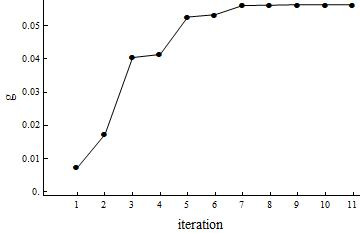
\includegraphics[scale =0.55] {DiscrApprox_G5.jpg}
   \label{GDevelDiscr}
 }
 \subfigure[Optimal strategy, $\mu=0.5$.]{
   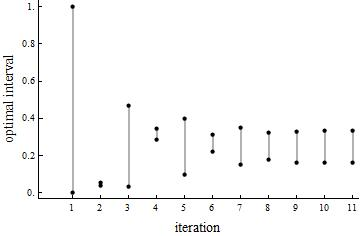
\includegraphics[scale =0.55] {DiscrApprox_Int5.jpg}
   \label{IDevelDiscr}
 }
  \subfigure[Growth rate of \texttt{CE}, $\mu=0.9$.]{
   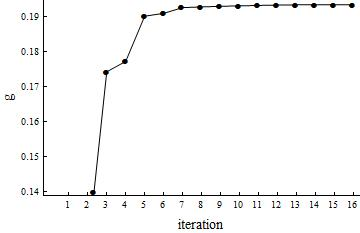
\includegraphics[scale =0.55] {DiscrApprox_G9.jpg}
   \label{GDevelCont}
 }
  \subfigure[Optimal strategy, $\mu=0.9$]{
   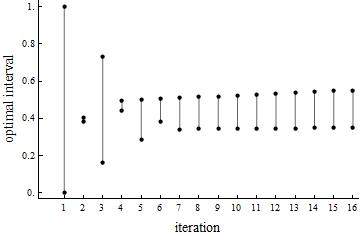
\includegraphics[scale =0.55] {DiscrApprox_Int9.jpg}
   \label{IDevelCont}
 }
\label{DiscrDevel}
\caption{Discrete time approximation, process of finding the optimal strategy.} %the parameters are $\mu=17$, $c=0.01$, $r=0.025$, $\sigma=0.5$ and $\gamma=1$.}
\end{figure}

\begin{figure}[ht!]
\centering
\subfigure[Growth rate of \texttt{CE}, $\mu=0.5$.]{
   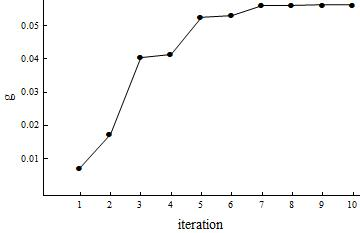
\includegraphics[scale =0.55] {ContApprox_G5.jpg}
   \label{GDevelDiscr}
 }
 \subfigure[Optimal strategy, $\mu=0.5$.]{
   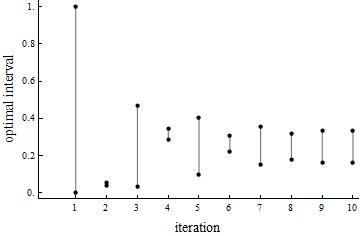
\includegraphics[scale =0.55] {ContApprox_Int5.jpg}
   \label{IDevelDiscr}
 }
  \subfigure[Growth rate of \texttt{CE}, $\mu=0.9$.]{
   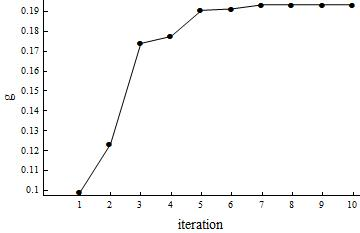
\includegraphics[scale =0.55] {ContApprox_G9.jpg}
   \label{GDevelCont}
 }
  \subfigure[Optimal strategy, $\mu=0.9$]{
   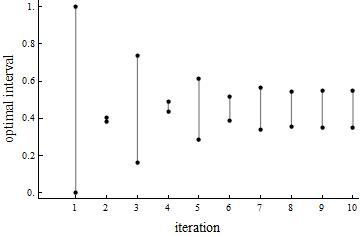
\includegraphics[scale =0.55] {ContApprox_Int9.jpg}
   \label{IDevelCont}
 }
\label{ContDevel}
\caption{Continuous time approximation, process of finding the optimal strategy.} %the parameters are $\mu=17$, $c=0.01$, $r=0.025$, $\sigma=0.5$ and $\gamma=1$.}
\end{figure}

\newpage

%Finally, we examine the dependance of optimal strategy on parameters of the model. We vary one parameter with the rest of the parameters fixed and we look at how the optimal interval changes. The figure \ref{Compr} shows the dependance on drift $\mu$, interest rate $r$, transaction costs $c$ and volatility $\sigma$ respectively. All the dependencies are in accordance with intuition. The higher is the drift, the more likely is the investor to hold his wealth in risky asset, so the optimal interval moves up. Opposite relation hold for interest rate $r$. With higher transaction cost the optimal interval becomes wider, which in consequence means less trading. With higher volatility of the risky asset the investor tends sharply to riskless asset.

\begin{comment}


\begin{figure}[ht]
\centering
\subfigure[]{
   \includegraphics[scale =0.45] {ComparativeMu.jpg}
   \label{ComprMu}
 }
 \subfigure[]{
   \includegraphics[scale =0.45] {ComparativeR.jpg}
   \label{ComprR}
 }
  \subfigure[]{
   \includegraphics[scale =0.45] {ComparativeC.jpg}
   \label{ComprC}
 }
  \subfigure[]{
   \includegraphics[scale =0.45] {ComparativeSigma.jpg}
   \label{ComprSigma}
 }
\label{Compr}
\caption{Dependance of optimal strategy on the parameters of the model, the fixed values of parameters are $\mu=17$, $c=0.01$, $r=0.025$, $\sigma=0.5$ and $\gamma=1$.}
\end{figure}
\end{comment}

%\chapter*{Conclusion}

%%%%%%%%%%%%%
%trading dynamics podla stanikovaj
\begin{comment}
\[V_t+b N^1_t S^1_t=V_t(1+c_{+} G_t)\]
remains the same before and after the transaction. In differential form we can write
\[\mathrm{d}^+ \log V_t=-\mathrm{d}^+\log(1+c_{+} G_t)=-\nu_+(G_t)\mathrm{d}^+ G_t,\]
where $\mathrm{d}^+$ represents the infinitesimal change caused by buying the stock and
\begin{equation}
\label{nuplus}
\nu_+(x)=\frac{c_{+}}{1+c_{+} x}.
\end{equation}
On the other hand if the investor sell the stock the quantity 
\[V_t-c N^1_t S^1_t=V_t(1-c_{-} G_t)\]
remains the same before and after the transaction. In differential form we can write
\[\mathrm{d}^- \log V_t=-\mathrm{d}^-\log(1-c_{-} G_t)=-\nu_-(G_t)\mathrm{d}^- G_t,\]
where $\mathrm{d}^-$ represents the infinitesimal change caused by buying the stock and
\begin{equation}
\label{numinus}
\nu_-(x)=\frac{c_{-}}{1-c_{-} x}.
\end{equation}
\end{comment}


%%%%%%%%%%%%%%%%%%%%%%%%%%%%%%%%%%%%%%%%%%%%%%%%%%%%%%%%%%%%%%%%%%%%%%%%
\begin{comment}
Now we add trading to the dynamics. Denote by $N_t^{+}$ and $N_t^{-}$ the sum of stocks bought and sold on the interval $[0,t)$ respectively. So the total number of socks $N^1_t$ is equal to $N_t^{+} - N_t^{-}$. We assume that the trading can be realized only in discrete time instances. That is, the processes $N_t^{+}$ and $N_t^{-}$ have piecewise constant trajectories. Buying $\mathrm{d}N_t^{+}$ or selling $\mathrm{d}N_t^{-}$ amount of stocks bears transaction costs equal to $c_{\pm}\,S_t\,\mathrm{d}N_t^{\pm}$. Putting this to \eqref{qv} we get
\begin{equation}
\label{qvv}
\mathrm{d}V_t=V_t\,[(r+(\mu-r)\,G_t)\,\mathrm{d}t+\sigma\,G_t\,\mathrm{d}W_t]-c_{+}\,S_t\,\mathrm{d}N_t^{+}+c_{-}\,S_t\,\mathrm{d}N_t^{-}.
\end{equation}

Using Ito's formula we gain
\begin{equation*}
V_t\,\mathrm{d} V_t^{-1} = -\frac{\mathrm{d}V_t}{V_t}+\frac{(\mathrm{d}V_t)^2}{V_t^2}=[-r-(\mu-r)\,G_t+\sigma^2\,G_t^2]\,\mathrm{d}t -\sigma\,G_t\,\mathrm{d}W_t + c_{\pm}\,V_t^{-1}\,\mathrm{d}^{\pm}N_t .
\end{equation*}
Once again, the technical details of the computation can be found in Appendix D. Realizing that $G_t=N_t^1\,S_t^1\,V_t^{-1}$, we compute {\color{red} (toto napisat prehladnejsie...)}

\begin{align*}
\mathrm{d} G_t&=(N_t^1\,V_t^{-1})\,\mathrm{d}S_t^1+(N_t^1\,S_t^1)\,\mathrm{d}V_t^{-1}+N_t^1\,(\mathrm{d}S_t^1)\,(\mathrm{d}V_t^{-1}) +(V_t^{-1}\,S_t^1)\mathrm{d}N_t^{\pm}\\
&=N_t^1\,V_t^{-1}\,(\mu\,S_t^1\,\mathrm{d}t+\sigma\,S+t^1 \mathrm{d}W_t) + N_t^1\,S_t^1\,V_t^{-1}[(-r(\mu-r)\,G_t+\sigma^2\,G_t^2)\mathrm{d}t+\\ 
&\quad -\sigma^2\,G_t\,\mathrm{d}W_t + c_{\pm}\,V_t^{-1}\,\mathrm{d}N_t^{\pm}] -N_t^1\,V_t^{-1}\,\sigma^2\,G_t\,S_t^1\,\mathrm{d}t +(V_t^{-1}\,S_t^1)\mathrm{d}N_t^{\pm} \\
&=G_t(\mu\mathrm{d}t+\sigma\mathrm{d}W_t)+G_t[(-r-(\mu-r)\,G_t+\sigma^2\,G_t^2)\,\mathrm{d}t-\sigma\,G_t\,\mathrm{d}W_t]-\sigma^2\,G_t^2\,\mathrm{d}t \\
&\quad c_{\pm}\,N_t\,S^1_t\,V_t^{-2}\,\mathrm{d}N_t^{\pm}+V_t^{-1}\,S_t^1\mathrm{d}N_t^{\pm}\\
&=G_t(\mu-r-(\mu-r)\,G_t-\sigma^2\,G_t^2-\sigma^2\,G_t)\,\mathrm{d}t + G_t\,(\sigma-\sigma\,G_t)\,\mathrm{d}W_t\\
&\quad +(1+c_{\pm}\,G_t)\,S_t\,V_t^{-1}\,\mathrm{d}N_t^{\pm}\\
&=G_t\,(1-G_t)[(\mu-r-\sigma^2\,G_t)\,\mathrm{d}t + \sigma\,\mathrm{d}W_t]+\mathrm{d}G_t^{\pm}.
\end{align*}
Define functions describing drift and volatility
\[b(x)=x\,(1-x)\,(\mu-r-\sigma^2\,x),\]
\[s(x)=\sigma\,x\,(1-x).\]
Now we can express the dynamics of $G_t$ as
\begin{equation}
\label{position}
\mathrm{d}G_t=b(G_t)\mathrm{d}t+s(G_t)\mathrm{d}W_t-\mathrm{d}^{\pm} G_t.
\end{equation}
\end{comment}

\addcontentsline{toc}{chapter}{\protect\numberline{}Conclusion}
\chapter*{Conclusion}

For both discrete time and continuous time Markov decision chains we developed the iterative algorithm for finding a control that maximizes
\begin{equation*}
\label{zaver}
\lim_{t\rightarrow\infty}\tfrac{1}{\gamma}\,t^{-1}\,\log(-\mathbb{E}[U_t]),
\end{equation*}
where $U_t$ is utility from reward over the time horizon $[0,t]$. The algorithm is numerically tractable. 

Both discrete time and continuous time version of algorithm were applied on a particular problem in portfolio optimization theory. It presents how a continuos time problem of optimal stochastic control can be solved numerically via Markov chain approximation. The method can be possibly applied for different problems. The results provide a sufficient consistency with the analytical solution, which demonstrate that they work properly.   

%demostrating a  for    in  works properly was applied

%The alghorthms was derive
%In the second chapter possible application of the alghorithm for continuous time problem was demostrated. By approximating 

%\appendix
%\renewcommand\chaptername{Appendix}
%\addcontentsline{toc}{chapter}{Appendices}
%\renewcommand\thesection{Appendix \Alph{section}}
\begin{appendices}

\chapter{Perron-Frobenius Theory}
In this section we summarize the results of Perron-Frobenius theory about non-negative matrices that is used throughout the thesis. Comprehensive explanation of the topic can be found in monograph by Lancaster and Tismenetsky \cite{Lancaster} in Chapter 15.

Let $\bm{A}$ be a square $n\times n$ matrix with non-negative entries. We denote this fact by $A\geq0$.
\begin{df}
Let $d_j$ be the greatest common divisor of those $m\geq1$ for which $\bm{A}^m_{jj}>0$. If $d_j=1$ for all $j=1,\dots,n$ then the matrix $\bm{A}$ is called {\em aperiodic}. 
\end{df}
\begin{df}
The square matrix $\bm{A}$ of order $n$ is called {\em irreducible} if for every permutation matrix $\bm{R}$
\[ \bm{R}\,\bm{A}\,\bm{R}^{-1}\neq\left( \begin{array}{cc}
\bm{C} & \bm{0}  \\
\bm{D} & \bm{F}  \\
\end{array} \right), \] 
where \bm{C} and \bm{F} are square matrices of order $2$ at least.
\end{df}
\noindent These terms are directly related to the same terms defined for Markov chains. If $X$ is a Markov chain with transition matrix $\bm{P}$, then $X$ is aperiodic iff \bm{P} is aperiodic, and $X$ is irreducible iff \bm{P} is irreducible.

\begin{thm}[Perron-Frobenius] 
\label{PF}
Let $\bm{A}$ be a nonnegative, irreducible and aperiodic square matrix. Then there exists a real eigenvalue $\lambda_1>0$ of $\bm{A}$, such that $\lambda_1>|\lambda|$ for all other eigenvalues of $\bm{A}$. Moreover, (right) eigenvector $\bm{v}$ respective to $\lambda_1$ can be chosen entrywise positive and $\text{ker}(\bm{A}-\lambda\bm{I})$ is onedimensional. The same holds for a left eigenvalue $\bm{w}$, that is for a eigenvector of $\bm{A}\tr$ respective to $\lambda_1$.
\end{thm}

\begin{thm} 
\label{PFlimit}
Let $\bm{A}$ be a nonnegative, irreducible and aperiodic square matrix. Let $\lambda>0$ be its maximal eigenvalue given by Perron-Frobenius theorem. Then
$$\lim_{k\rightarrow\infty}{\lambda^{-k}}\bm{A}^k=\frac{\bm{v}\,\bm{w}\tr}{\bm{v}\tr\,\bm{w}}$$%=\bm{v}\,\frac{\sum_{i} w_i}{\sum_i v_i\, w_i}=k(\bm{v},\bm{w})\,\bm{v},$$
where $\bm{v}$ is any right eigenvector and $\bm{w}$ is any left eigenvector of $\bm{A}$ respective to $\lambda$. %If $\bm{v}$ is choosen positive, then the constant $k(\bm{v},\bm{w})$ is also positive.
\end{thm}
Note that if $\bm{v}$ is chosen positive, then 
$$\lim_{k\rightarrow\infty}{\lambda^{-k}}\bm{A}^k\,\bm{1}=\frac{\sum_{i} w_i}{\sum_i v_i\, w_i}\,\bm{v}=k(\bm{v},\bm{w})\,\bm{v},$$
where $k(\bm{v},\bm{w})$ is a positive constant.

\begin{thm}
\label{ineq}
Let $\bm{A}$ be a nonnegative, ireducible square matrix. Let $\lambda>0$ be its maximal eigenvalue and let $\bm{v}$ be a positive vector. Then following inequality holds
\begin{equation*}
\min_i \frac{\sum_j a_{ij}\,v_j}{v_i}\leq\lambda\leq\max_i \frac{\sum_j a_{ij}\,v_j}{v_i}
\end{equation*}
and the inequality with equality sign holds if and only if $\bm{v}$ is an eigenvector of $\bm{A}$ respective to $\lambda$.
\end{thm} 

\begin{comment}
\begin{lem}
\label{TtoS}
Let \bm{S}=\exp{\bm{T}}. Let $\kappa_1$ be a maximal egenvalue of $\bm{T}$, that is the one with maximal Eeuclidean norm. Then $e^{\kappa_1}=\lamba_1$ is a maximal eigenvalue of $\bm{S}$. Moreover eigenspace of $\bm{T}$ corresponding to $\mu$ coincides with eigenspace of $\bm{S}$ corresponding to $\lambda$
\end{lem}
\begin{proof}
Note that the 
$$\mu^a=\underset{u\in\mathcal{A}}{\operatorname{argman}}\|{mu|\}$$
\end{proof}
\end{comment}

\chapter{Matrix Exponential Function}

Here we summarize some facts about the matrix exponential that we used in Section 1.5. Particularlly, we are interested in its eigenvalues and eigenvectors.

Let $\bm{A}$ be a square $n \times n$ matrix. Define a matrix function on $[0,\infty)$ by
\begin{equation}
\label{MexpDef}
\exp\{u\,\bm{A}\}\triangleq \sum_{k=0}^{\infty}\frac{(u\,\bm{A})^k}{k!}.
\end{equation}  
We will assume that $\bm{A}$ has $n$ distinct eigenvalues $\lambda_1,\dots,\lambda_n$, i.e. the Jordan canonical form of \bm{A} is of the form
\[\bm{D}\triangleq\text{diag}(\{\lambda_i\}).\]
This simplifying assumtion hepls us to clearly demonstrate the idea behind. However, note that all the results that will be stated hold also for general case. The methods used for general case are similar, but considering the general Jordan canonical form the notation becomes more technical. For fully rigorous treatment see \cite{Baker}. 

%form assumtion demostrate the idea All the result ho is similar but more technical considering However all the result holds hold for all the results Suppose that $\bm{A}$ has $n$ distinct eigenvalues $\lambda_1,\dots,\lambda_n$. Denote the Jordan form of the matrix $\bm{A}$ by $\bm{D}$. That is, there exists a regular matrix $\bm{P}$ such that 
%\[\bm{A}=\bm{P}\,\bm{D}\,\bm{P}^{-1}, \quad \bm{D}=\text{diag}(\{\lambda_i\}).\] demostrate the The crucial result for us is that matrix exponential leaving the corresponding eigenspace unchanged is that

Using the Jordan canonical form the matrix $\bm{A}$ can be decomposed to $\bm{P}\,\bm{D}\,\bm{P}^{-1}$ for some matrix $\bm{P}$.  Note that 
\[\bm{A}^2=\bm{P}\,\bm{D}\,\bm{P}^{-1}\,\bm{P}\,\bm{D}\,\bm{P}^{-1}=\bm{P}\,\bm{D}^2\,\bm{P}^{-1}.\]
So by induction we have $\bm{A}^k=\bm{P}\,\bm{D}^k\,\bm{P}^{-1}$ for $k\in\mathbb{N}$. Then the power series in \ref{MexpDef} can be expressed as
\begin{align*}
\exp\{u\,\bm{A}\}&= \sum_{k=0}^{\infty}\frac{1}{k!}u^k\,\bm{P}\,\bm{D}^k\,\bm{P}^{-1}\\
&=\bm{P}\,\left(\sum_{k=0}^{\infty}\frac{u^k\,\bm{D}^k}{k!}\right)\,\bm{P}^{-1}\\
&=\bm{P}\,\exp\{u\,\bm{D}\}\,\bm{P}^{-1},
\end{align*}
where
\[\exp\{u\,\bm{D}\}\triangleq\text{diag}(\{e^{u\,\lambda_i}\}).\]
This shows the existence of $\exp\{u\,\bm{A}\}$. As $\exp\{u\,\bm{D}\}$ is the Jordan canonical form of $\bm{D}$, the eigenvalues of $\bm{D}$ are $e^{u\,\lambda_1},\dots,e^{u\,\lambda_n}$. 
Moreover, if $\bm{v}$ is an eigenvector of $\bm{A}$ corresponding to $\lambda_i$, then
\[\exp\{u\,\bm{A}\}\bm{v}=\sum_{k=0}^{\infty}\frac{u^k\,\bm{A}^k\,\bm{v}}{k!}=\sum_{k=0}^{\infty}\frac{u^k\,\lambda_i^k\,\bm{v}}{k!}=e^{\lambda_i}\,\bm{v}.\]
Consequently, the eigenspace of $\bm{A}$ corresponding to $\lambda_i$ is identical to the eigenspace of $\exp\{\bm{A}\}$ corresponding to $e^{\lambda_i}$. 

%matrix is replaced by general Jordan form matrix
%the eigenvalues of the matrix $\bm{D}$ $\exp\{u\,\bm{A}\}$.
%spectrum of $\\bm{A}$
%All results holds.. technical, see..  

\chapter{A Matrix Result}

Here is the technical Lemma that is used in the proof of the Proposition \ref{propC}. The idea behind the proof is just a direct use of Taylor expansion.

We start with the definition of a matrix norm that we will use.
\begin{df}
Let $\bm{A}$ be a square $n \times n$ matrix. Define the matrix \textit{operator norm} by
\[\left\|\bm{A}\right\|=\max\{ \left\|\bm{A}\,\bm{x}\right\|:\left\|\bm{x}\right\|\leq 1\},\]
where $\bm{x}\in\mathbb{R}^n$ and $\left\|\bm{x}\right\|=\underset{i}{\max} \,|x_{i}|$.
\end{df}
\noindent For any non-zero vector $\bm{x}$ we have $\|\bm{A}\,\tfrac{\bm{x}}{\left\|\bm{x}\right\|}\|\leq \left\|\bm{A}\right\|$ and thus $\left\|\bm{A}\,\bm{x}\right\|\leq \left\|\bm{A}\right\|\left\|\bm{x}\right\|$. Employing this inequality we get
\[\left\|\bm{A}\,\bm{B}\,\bm{x}\right\|\leq\left\|\bm{A}\right\|\,\left\|\bm{B}\,\bm{x}\right\|\leq\left\|\bm{A}\right\|\,\left\|\bm{B}\right\|\,\left\|\bm{x}\right\|,\]
and consequently
\begin{equation}
\label{ineq}
\left\|\bm{A}\,\bm{B}\right\|\leq \left\|\bm{A}\right\|\,\left\|\bm{B}\right\|.
\end{equation}

%Now we proceed to the Lemma.
%\begin{prop}

%\end{prop}

\begin{lem}
\label{MatrixResult}
Let $\bm{A}$, $\bm{B}$ and $\bm{C}$ be square $n \times n$ matrices. Let entries of the main diagonal of the matrix $\bm{C}$ be equal to $1$, e.i. $c_{ii}=1$. Then
$$\lim_{n\rightarrow\infty}\left[\big(\exp\{\tfrac{1}{n}\,\bm{A}\}\cdot\exp\{\tfrac{1}{n}\,\bm{B}\}\big) \ast \bm{C}\right]^n=\exp\{(\bm{A}+\bm{B})\ast\bm{C}\}.$$
%$$[\exp\{\tfrac{1}{n}\,\bm{A}\ast \bm{B}\}]^n\longrightarrow \exp\{\bm{A}\ast\bm{B}\}, \quad n\longrightarrow\infty.$$
\end{lem}
\begin{proof}

1) First we show that the exponential $\exp\{\tfrac{1}{n}\,\bm{A}\}$ can be well approximated by $\bm{I}+\tfrac{1}{n}\,\bm{A}$, meaning that
\begin{equation}
\label{AppB1}
\exp\{\tfrac{1}{n}\,\bm{A}\}=\bm{I}+\tfrac{1}{n}\,\bm{A}+O\left(\tfrac{1}{n^2}\right), \quad n\longrightarrow\infty.
\end{equation}
It is sufficient to show that $\bm{H}(t)=t^{-2}(\exp\{\bm{A}t\}-\bm{I}-\bm{A}\,t)$ converges to some finite matrix as $t$ goes to zero. Using L' Hospital's rule twice we get
$$\frac{d\,\bm{H}(t)}{d^2\,t}=\tfrac{1}{2}\,\bm{A}^2\,\exp\{\bm{A}\,t\}\longrightarrow\tfrac{1}{2}\,\bm{A}^2, \quad t\longrightarrow 0.$$
2) The relation \eqref{AppB1} implies
\begin{equation}
\label{AppB2}
\exp\{\tfrac{1}{n}\,\bm{A}\}\cdot\exp\{\tfrac{1}{n}\,\bm{B}\}=\bm{I}+\tfrac{1}{n}\,(\bm{A}+\bm{B})+O\left(\tfrac{1}{n^2}\right), \quad n\longrightarrow\infty.
\end{equation}
3) Because the main diagonal of the matrix $\bm{C}$ consists of ones, we have $\bm{I}\ast\bm{C}=\bm{I}$. Thus, using the relation \eqref{AppB2} for $n$ going to infinity
\begin{equation}
\label{AppB3}
\begin{split}
\big(\exp\{\tfrac{1}{n}\,\bm{A}\}\cdot \exp\{\tfrac{1}{n}\,\bm{B}\}\big)\ast \bm{C}&=\left[\bm{I}+\tfrac{1}{n}\,(\bm{A}+\bm{B})+O\left(\tfrac{1}{n^2}\right)\right]\ast\bm{C}\\
&=\bm{I}+\tfrac{1}{n}\,\bm{E}+O\left(\tfrac{1}{n^2}\right),
\end{split}
\end{equation}
where $\bm{E}=(\bm{A}+\bm{B})\ast\bm{C}$.\\
4) Finally we show the convergence. Define sequence
\[ \bm{D}_n=\big(\exp\{\tfrac{1}{n}\,\bm{A}\}\cdot \exp\{\tfrac{1}{n}\,\bm{B}\}\big)\ast \bm{C}-\bm{I}+[\tfrac{1}{n}\,[(\bm{A}+\bm{B})\ast\bm{C}]], \]
which is according to \eqref{AppB3} $O\left(\tfrac{1}{n^2}\right)$. Using the binomial theorem we get 
\begin{align*}
\left[\big(\exp\{\tfrac{1}{n}\,\bm{A}\}\cdot\exp\{\tfrac{1}{n}\,\bm{B}\}\big)\ast \bm{C}\right]^n&=[(\bm{I}+\tfrac{1}{n}\,(\bm{A}+\bm{B})\ast\bm{C})+\bm{D}_n]^n\\
&=\left[\bm{I}+\tfrac{1}{n}\,\bm{E}\right]^n+\sum_{k=1}^n {{n}\choose{k}}\,\bm{D}_n^k\,\left(\bm{I}+\tfrac{1}{n}\bm{E}\right)^{n-k}.
\end{align*}
We tend to show that the second term is negligible. 
Then using the triangle inequality and \eqref{ineq} we get
%, because the term $[\bm{I}+\tfrac{1}{n}(\bm{A}\ast\bm{B})]^{n-k}$ converges to a finite limit and
%\[ \sum_{k=1}^n {{n}\choose{k}}\,\bm{C}_n^k \leq \sum_{k=1}^n \frac{n^k}{k!}\,\bm{C}_n^k=o(1) \]
\begin{align*}
\left\|\sum_{k=1}^n {{n}\choose{k}}\,\bm{D}_n^k\,\left(\bm{I}+\tfrac{1}{n}\bm{E}\right)^{n-k}\right\|
&\leq \sum_{k=1}^n {{n}\choose{k}}\,\left\|\bm{D}_n\right\|^k\,\left(\left\|\bm{I}\right\|+\tfrac{1}{n}\left\|\bm{E}\right\|\right)^{n-k}\\
&=\left\|\bm{D}_n\right\|\,\sum_{l=0}^{n-1} {{n-1}\choose{l+1}}\,\left\|\bm{D}_n\right\|^l\,\left(1+\tfrac{1}{n}\left\|\bm{E}\right\|\right)^{n-1-l}\\
&\leq n\,\left\|\bm{D}_n\right\|\,\sum_{l=0}^{n-1} {{n-1}\choose{l}}\,\left\|\bm{D}_n\right\|^l\,\left(1+\tfrac{1}{n-1}\left\|\bm{E}\right\|\right)^{n-1-l}\\
&=(n\,\left\|\bm{D}_n\right\|)\,(1+\left\|\bm{D}_n\right\|+\tfrac{1}{n-1}\left\|\bm{E}\right\|)^{n-1}.  
\end{align*}
First factor converges to $0$ as $\bm{D}_n$ is $O(\tfrac{1}{n^2})$. The second term converges to $\exp\{\left\|\bm{E}\right\|\}$, e.i. finite number. Thus the whole term converges to $0$. 
%The second summand is negligible, 
%\begin{align*} \sum_{k=1}^n {{n}\choose{k}}\, O\left(\tfrac{1}{n^2}\right)^k\, \left(\bm{I}+\tfrac{1}{n}(\bm{A}\ast\bm{B})\right)^{n-k}&=\sum_{k=1}^n \tfrac{n\,(n-1)\dots(n-k+1)}{k!} \, O\left(\tfrac{1}{n^{2k}}\right)\,O(1)\\
%&\leq \sum_{k=1}^n \tfrac{n^k}{k!}\, O\left(\tfrac{1}{n^{2k}}\right)=\sum_{k=1}^n O\left(\tfrac{1}{n^k}\right)=o(1).
%\end{align*}
We can conclude
\begin{align*}
\left[\big(\exp\{\tfrac{1}{n}\,\bm{A}\}\cdot\exp\{\tfrac{1}{n}\,\bm{B}\}\big)\ast \bm{C}\right]^n&=[(\bm{I}+\tfrac{1}{n}\,(\bm{A}+\bm{B})\ast\bm{C})]^n+o(1)\\
&\longrightarrow\exp\{(\bm{A}+\bm{B})\ast\bm{C}\},\quad n\longrightarrow\infty.\qedhere
\end{align*}
%\begin{align*}
%$$ \sum_{k=1}^n {{n}\choose{k}}\, O\left(\tfrac{1}{n^2}\right)^k\, \left(\bm{I}+\tfrac{1}{n}(\bm{A}\ast\bm{B})\right)^{n-k}=\sum_{k=1}^n \tfrac{n\,(n-1)\dots(n-k+1)}{k!} \, O\left(\tfrac{1}{n^2k}\right)\,\left(\bm{I}+\tfrac{1}{n}(\bm{A}\ast\bm{B})\right)^{n-k}  $$
%\leq \sum_{k=1}^n \frac{n^k}{k!} \, %O\left(\tfrac{1}{n^2}\right)^k\,\left(\bm{I}+\tfrac{1}{n}(\bm{A}\ast\bm{B})\right)^{n-k}\\
%&=22
%\end{align*}
\end{proof}

\chapter{Stochastic calculus}
In this section we only introduce basic stochastic calculus tools that we use in Chapter 2. These are Ito's formula for computing the differential of a process and Girsanov Theorem. The whole stochastic calculus is a complex mathematical theory while deeper insight is out of the scope of this thesis. Readable but sufficiently rigorous explanation of the topic can be found for instance in monograph \cite{Shreve}.\\
%quadratic variation
%Ito
\begin{thm}[Ito's Formula] 
\label{ItoThm}
Let $f:\mathbb{R}\rightarrow\mathbb{R}$ be a twice continuously differentiable function and let $X=(X_t,t\geq0)$ be a real-valued continuous semimartingale. Then
\begin{equation}
\label{ItoFormula}
f(X_t)=f(X_0)+\int_0^t f^{\prime}(X_s)\mathrm{d}X_s+\int_0^t f^{\prime\prime}(X_s)\mathrm{d}\langle X,X \rangle_s.
\end{equation}
%$\int_{0}^t X_s \mathrm{d} < \infty$ almost surely for all $t>0$.
\end{thm}
\noindent We can reformulate the equation \eqref{ItoFormula} using the differential notation in a following way,
\begin{equation}
\label{ItoFormula2}
\mathrm{d}f(X_t)=f^{\prime}(X_t)\mathrm{d}X_t+f^{\prime\prime}(X_t)\mathrm{d}\langle X\rangle_t.
\end{equation}
Here are the two applications of \eqref{ItoFormula2} that are used in the Chapter 2.
\begin{enumerate}
\item For $f(x)=\ln(x)$ we have $f^{\prime}(x)=x^{-1}$, $f^{\prime\prime}(x)=-x^{-2}$ and
\[\mathrm{d}\ln(X_t)=\frac{\mathrm{d}X_t}{X_t}-\frac{\mathrm{d}\langle X\rangle_t}{2X_t^2}.\]
\item For $f(x)=x^{-1}$ we have $f^{\prime}(x)=-x^{-2}$ $f^{\prime\prime}(x)=2 x^{-3}$ and
\[\mathrm{d}X_t^{-1}=-\frac{\mathrm{d}X_t}{X_t^2}+\frac{\mathrm{d}\langle X\rangle_t}{X_t^2}.\]
\end{enumerate}

\begin{comment}
\begin{thm}[Girsanov Theorem] 
\label{Girsanov}
Let $\{\Omega,\mathcal{F},\mathbb{P}\}$ be a probability space with Brownian motion $W_t$. Let be $\{\mathcal{F}_t^{W}\}$ the filtration generated by the Brownian motion $W$. Let $(X_t,t\geq 0)$ be an $\{\mathcal{F}_t^{W}\}$-martingale with bounded trajectories.
%\[\mathbb{E}[\exp\{\int_0^t X^2_t \mathrm{d}\}]<\infty, \quad \text{for all } t>0. \]
 Define stochastic exponential $\mathcal{E}(X)$ by
\[\mathcal{E}(X)_t=\exp\{X_t-\tfrac{1}{2}\left\langle X \right\rangle_t\}.\]
Then for any fixed $T>0$ there exist a measure $\mathbb{Q}_{T}$ such that
\[\frac{\mathrm{d}\mathbb{Q}_T}{\mathrm{d}\mathbb{P}}|_{\mathcal{F}_t^{W}}=\mathcal{E}(X)_t,\quad 0\leq t\leq T.\] %\restriction
Moreover
\[\widetilde{W}_t=W_t-\left\langle W,X \right\rangle_t,\quad 0\leq t\leq T.\]
is a Brownian motion under the measure $\mathbb{Q}_T$.
\end{thm}
\end{comment}

We say that the process $G$ satisfies \textit{Novikov condition} on $[0,T]$ if
\begin{equation}
\mathbb{E}\left[\exp\Big(\frac{1}{2}\int_0^T G^2_s \,\mathrm{d}s \Big)\right]<\infty.
\end{equation}

\begin{thm}[Girsanov Theorem] 
\label{Girsanov}
Let $(\Omega,\mathcal{F},(\mathcal{F}_t),\mathbb{P})$ be a filtrated probability space satisfying usual conditions (UC). Let $W$ be an ($\mathcal{F}_t$)-martingale and let  $G_t$ be an ($\mathcal{F}_t$)-progressively measeruble process satisfying Novikov condition on every interval $[0,T]$. Put 
\[X\triangleq\int_0^t G_s \,\mathrm{d}W_s.\]
%Brownian motion $W_t$. Let be $\{\mathcal{F}_t^{W}\}$ the filtration generated by the Brownian motion $W$. Let $(X_t,t\geq 0)$ be an $\{\mathcal{F}_t^{W}\}$-martingale with bounded trajectories.
%\[\mathbb{E}[\exp\{\int_0^t X^2_t \mathrm{d}\}]<\infty, \quad \text{for all } t>0. \]
 Define stochastic exponential $\mathcal{E}(X)$ by
\[\mathcal{E}(X)_t\triangleq\exp\{X_t-\tfrac{1}{2}\left\langle X \right\rangle_t\}.\]
Then for any fixed $T>0$ there exist a measure $\mathbb{Q}_{T}$ such that
\[\frac{\mathrm{d}\mathbb{Q}_T}{\mathrm{d}\mathbb{P}}|_{\mathcal{F}_T}=\mathcal{E}(X)_T.\] %\restriction
Moreover
\[\widetilde{W}_t=W_t-\left\langle W,X \right\rangle_t,\quad 0\leq t\leq T.\]
is a Brownian motion under the measure $\mathbb{Q}_T$.
\end{thm}

\end{appendices}


%\chapter{The Program Implementation}   

We implemented continuous time and discrete time alghoritms in Wolfram Mathematica 7.0. Here is the code for both procedures.\\
\\

%%%%%%%%%%%%%%%%%%%%%%%%%%%%%%%%%%%%%%%%%%%%%%%%%%%%%%
\begin{scriptsize}

h = 0.005; dt = 0.0001; n = 1/h + 1; G = Range[0, 1, h];\\
\\
ArgMinList[list2d\_] := Module[\{min, argument, values, output\},
  \begin{addmargin}[1em]{0em}
  argument = list2d[[All, 1]];\\
  values = list2d[[All, 2]];\\
  min = Min[values];\\
  If[Count[values, min] == 1, output = argument[[Position[values, min][[1, 1]]]], output = Null];\\
  output
  \end{addmargin} 
]\\
\\
\\
ModelDiscrete[r\_, mu\_, sigma\_, c\_, gamma\_] :=  Module[\{A, B, EigenA, lA, vA\},\\

  \begin{addmargin}[1em]{0em}
  (*portfolio drift and volatility*)\\
  b[x\_] := x (1 - x) (mu - r - (sigma\textasciicircum 2) x);\\
  s[x\_] := sigma x (1 - x);\\
  \\
  (*transition matrix*)\\
  PUp[g\_] := (h b[g] dt + (s[g])\textasciicircum 2 dt )/(2 h\textasciicircum 2);\\
  PDown[g\_] := (-h b[g] dt + (s[g])\textasciicircum 2 dt )/(2 h\textasciicircum 2);\\
  PZero[g\_] := 1 - (PUp[g] + PDown[g]) ;\\
  PRowUp[g\_] := Join[Table[0, \{g/h\}], \{PDown[g], PZero[g], PUp[g]\}, Table[0, \{n - g/h - 3\}]];\\
  PRowDown[g\_] := Join[Table[0, \{g/h - 2\}], \{PDown[g], PZero[g], PUp[g]\}, Table[0, \{n - (g/h - 2) - 3\}]];\\
  PRowZero[g\_] := Join[Table[0, \{g/h - 1\}], \{PDown[g], PZero[g], PUp[g]\}, Table[0, \{n - (g/h - 1) - 3\}]];\\
  PRow[a\_, g\_] := Piecewise[\{\{PRowZero[g], a == 0\}, \{PRowUp[g], a == 1\}, \{PRowDown[g], a == -1\}\}];\\
  \\
  (*rewards*)\\
  RZero[g\_] := (mu + (mu - r) g - 1/2 sigma\textasciicircum 2 g\textasciicircum 2) dt;\\
  rew[a\_, g\_] :=  Piecewise[\{\{RZero[g] - Abs[Log[1 - c g] - Log[1 - c (g - h)]], a == -1\}, \{RZero[g],
      \begin{addmargin}[1em]{0em} 
      a == 0\}, \{RZero[g] - Abs[Log[1 - c g] - Log[1 - c (g + h)]], a == 1\}\}];
      \end{addmargin}
  RRow[a\_, g\_] := Table[rew[a, g], \{n\}];\\
  \\
  (*interval - policy vector  transformation*)\\
  aVec[alpha\_, beta\_] := Join[Table[1, \{Round[(alpha + h)/h]\}], Table[0, \{Round[(beta - alpha)/h - 1]\}], Table[-1, \{Round[n - beta/h]\}]];\\
  aInt[aVec\_] := Union[h (Last[Position[aVec, 1]] - 1), h (First[Position[aVec, -1]] - 1)];\\
  \\
  (*S matrix*)\\
  SRow[a\_, g\_] := PRow[a, g] Exp[-gamma RRow[a, g]];\\
  S[aVec\_] := MapThread[SRow, \{aVec, G\}];\\
  \\
  (*iterative algorithm*)\\
  A = \{\};\\
  B = aVec[0, 1]; (*initial policy*)\\
  LambdaImprovement = \{\};\\
  PolicyImprovement = \{B\};\\
  While[A != B,
     \begin{addmargin}[1em]{0em}
     A = B;\\
     B = Table[Null, \{n\}];\\
     EigenA = Eigensystem[S[A], 1];\\
     lA = EigenA[[1, 1]];\\
     vA = EigenA[[2, 1]];\\
     vA = vA/Last[vA];\\
     B[[1]] = 1;\\
     B[[2]] = ArgMinList[\{\{0, SRow[0, h].vA\}, \{1, SRow[1, h].vA\}\}];\\
     For[k = 2, k <= n - 3, k++,
      \begin{addmargin}[1em]{0em}
      B[[k + 1]] = ArgMinList[\{\{-1, SRow[-1, k h].vA\}, \{0, SRow[0, k h].vA\}, \{1, SRow[1, k h].vA\}\}];
      \end{addmargin}
      ];\\
     B[[n - 1]] = ArgMinList[\{\{-1, SRow[-1, (n - 2) h].vA\}, \{0, SRow[0, (n - 2) h].vA\}\}];\\
     If[B[[n - 1]] == Null, B[[2]] = A[[2]]];\\
     B[[n]] = -1;\\
     For[k = 1, k <= n, k++, If[B[[k]] == Null, B[[k]] = A[[k]]]];\\
     PolicyImprovement = Append[PolicyImprovement, B];\\
     LambdaImprovement = Append[LambdaImprovement, lA];
     \end{addmargin}
  ]\\   
  LambdaImprovement = Append[LambdaImprovement, Eigensystem[S[B], 1][[1, 1]]];\\
  aInt[PolicyImprovement[[-1]]]
  ]  
  \end{addmargin} 
   
\end{scriptsize}
\vspace{0.7cm}

%%%%%%%%%%%%%%%%%%%%%%%%%%%%%%%%%%%%%%%%%%%%%%%%%%%%%%%%%%%%%%%%%%%%%%%%%%%%%%%%%%%%%%%%%% 
\begin{scriptsize} 

ModelContinuous[r\_, mu\_, sigma\_, c\_, gamma\_] := Module[\{A, B, EigenA, lA, vA\},\\

  \begin{addmargin}[1em]{0em}
  (*portfolio drift and volatility*)\\
  b[x\_] := x (1 - x) (mu - r - (sigma\textasciicircum 2) x);\\
  s[x\_] := sigma x (1 - x);\\
  \\
  (*transition rate matrix*)\\
  QUp[g\_] := (h b[g]  + (s[g])\textasciicircum 2  )/(2 h\textasciicircum 2);\\
  QDown[g\_] := (-h b[g]  + (s[g])\textasciicircum 2  )/(2 h\textasciicircum 2);\\
  QZero[g\_] := -(QUp[g] + QDown[g]);\\
  Qmove[g\_] := 100000;\\
  QRowZero[g\_] :=Join[Table[0, \{g/h - 1\}], \{QDown[g], QZero[g], QUp[g]\}, Table[0, \{n - Max[(g/h - 1), 0] -3\}]];\\
  QRowUp[g\_] := Join[Table[0, \{g/h\}], \{-Qmove[g], Qmove[g]\}, Table[0, \{n - Max[(g/h - 0), 0] - 2\}]];\\
  QRowDown[g\_] := Join[Table[0, \{g/h - 1\}], \{Qmove[g], -Qmove[g]\}, Table[0, \{n - Max[(g/h - 1), 0] - 2\}]];\\
  QRow[a\_, g\_] := Piecewise[\{\{QRowZero[g], a == 0\}, \{QRowUp[g], a == 1\}, \{QRowDown[g], a == -1\}\}];\\
  \\
  (*rewards*)\\
  revZero[g\_] := (mu + (mu - r) g - 1/2 sigma\textasciicircum 2 g\textasciicircum 2) dt;\\
  rev[a\_, g\_] := Piecewise[\{\{revZero[g] - Abs[Log[1 - c g] - Log[1 - c (g - h)]], a == -1\}, \{revZero[g],
    \begin{addmargin}[1em]{0em}
    a == 0\}, \{revZero[g] - Abs[Log[1 - c g] - Log[1 - c (g + h)]], a == 1\}\}];
    \end{addmargin}
  RVector[aVec\_] := MapThread[rev, \{aVec, G\}];\\
  RRow[a\_, g\_] :=  Join[Table[0, g h], rev[a, g], Table[0, n - g h - 1]];\\
  \\
  (*interval - policy vector  transformation*)\\
  aVec[alpha\_, beta\_] := Join[Table[1, \{Round[(alpha + h)/h]\}], Table[0, \{Round[(beta - alpha)/h - 1]\}],\\ 
    Table[-1, \{Round[n - beta/h]\}]];\\
  aInt[aVec\_] :=  Union[h (Last[Position[aVec, 1]] - 1), h (First[Position[aVec, -1]] - 1)];\\
  \\
  (*S matrix*)\\
  Q[aVec\_] := MapThread[QRow, \{aVec, G\}];\\
  T[aVec\_] := Q[aVec] - gamma DiagonalMatrix[RVector[aVec]];\\
  S[aVec\_] := MatrixExp[aVec];\\
  SRow[aVec, g\_] := S[aVec\_][[g h + 1, All]];\\
  \\
  (*iterative algorithm*)\\
  A = \{\};\\
  B = aVec[0, 1]; (*initial policy*)\\
  LambdaImprovement = \{\};\\
  PolicyImprovement = \{B\};\\
  While[A != B,
     \begin{addmargin}[1em]{0em}
     A = B;\\
     B = Table[Null, \{n\}];\\
     EigenA = Eigensystem[S[A], 1];\\
     lA = EigenA[[1, 1]];\\
     vA = EigenA[[2, 1]];\\
     vA = vA/Last[vA];\\
     B[[1]] = 1;\\
     B[[2]] = ArgMinList[\{\{0, SRow[0, h].vA\}, \{1, SRow[1, h].vA\}\}];\\
     For[k = 2, k <= n - 3, k++,
      \begin{addmargin}[1em]{0em}
      B[[k + 1]] = ArgMinList[\{\{-1, SRow[-1, k h].vA\}, \{0, SRow[0, k h].vA\}, \{1, SRow[1, k h].vA\}\}];\\
      ];
      \end{addmargin}
     B[[n - 1]] = ArgMinList[\{\{-1, SRow[-1, (n - 2) h].vA\}, \{0,SRow[0, (n - 2) h].vA\}\}];\\
     If[B[[n - 1]] == Null, B[[2]] = A[[2]]];\\
     B[[n]] = -1;\\
     For[k = 1, k <= n, k++, If[B[[k]] == Null, B[[k]] = A[[k]]]];\\
     PolicyImprovement = Append[PolicyImprovement, B];\\
     LambdaImprovement = Append[LambdaImprovement, lA];\\
     ]\\
     \end{addmargin}   
    LambdaImprovement =  Append[LambdaImprovement, Eigensystem[S[B], 1][[1, 1]]];\\
  aInt[PolicyImprovement[[-1]]]\\
  ]\\
  \end{addmargin}
\end{scriptsize}

\end{appendices}

\clearpage 
%\addcontentsline{toc}{chapter}{Literat�ra}
\begin{thebibliography} {99}
 %\addcontentsline{toc}{section}{Literatura}

\bibitem{Baker} Baker A., (2006), ``Matrix Groups: An Introduction to Lie Group Theory'', 3rd edition, Princeton Springer Great Britain.  
\bibitem{Bellman} Bellman R.E., (1957), ``Dynamic Programming'', Princeton University Press, NJ. 
\bibitem{Benchmark} Bielicky T.R., Chancelier J. P., Pliska S. R., Sulem A., (2003), ``Risk sensitive portfolio optimization with transaction cost'', {\em Journal of Computational Finance, 8(1), 39-63}. 
\bibitem{Benchmark2} Bielicky T.R., Pliska S. R., (2000), ``Risk sensitive dynamic asset management in the presence of transaction costs'', {\em Finance and Stochastics}, vol. 4, pp. 1-33. 
\bibitem{survey} Cadenilas A., (2000), ``Consumption-investment problems with transaction cost: survey and open problems,'', {\em Math. Methods Operations Research, vol 51}, pp,43-68. 
\bibitem{Dostal} Dost�l P., ``Investment strategies in the long run with proportional transaction costs and a HARA utility function'',{\em Quantitative Finance, Vol. 9, No. 2, March 2009}.
\bibitem{MP} Ethier N., Kurtz G., (2005), ``Markov Processes'', John Wiley \& Sons, New Jersey. 
\bibitem{Portfolio} Follmer H., Schied A., (2004), ``Stochastic Finance. An Introduction in Discrete Time'', second edition, Walter de Gruyter, Berlin
\bibitem{Howard} Howard  R.A., (1972), ``Dynamic Programming and Markov Processes'', {\em Management Science}, Vol. 18, No. 7, March 1972.
\bibitem{HowardRS} Howard  R.A., Matheson J.E., (1960), ``Risk-Sensitive Markov Decision pocesses'', The M.I.T. Press, Princeton, NJ.
\bibitem{Howard} Howard R.A, Metheson J.E., (1972), ``Risk-Sensitive Markov Decision Processes'',. {\em Management Science}, Vol. 18, No. 7, March.   
\bibitem{Praskova} Karlin S., Taylor H.M., (1981), ``A Second Course in Stochastic Processes'', 
Academic Press, New York.
%\bibitem{Kal} Kalu��kov� M., ``Diskontovan� ��zen� portfolia'', Bachelor thesis {\em MFF UK}
\bibitem{KushnerDupuis} Kushner H.J., Dupuis P., (2001), ``Numerical Methods for Stochastic Control Problems in Continuous Time'',  Springer-Verlag, New York .  
\bibitem{Lancaster} Lancaster P., Tismenetsky M., (1985), ``The Theory of Matrices Second Edition'',  Academic Press.
\bibitem{Liggett} Liggett T.M., (2010), ``Continuous Time Markov Processes: An Introduction'',  American Mathematical Society, Providence.
\bibitem{MC} Norris J.R., (1997), ``Markov Chain'', Cambridge University Press, Cambridge. 
\bibitem{Merton} Merton R.C., (1992), ``Continuous-Time Finance'', B. Blackwell.
\bibitem{Shreve} Shreve S.E., (1981), ``Stochastic Calculus for Finance II'', Springer, New York.
\bibitem{Sta} Stan�kov� D. (2006), ``Asymptotic Control of Portfolio'', Bachelor thesis, MFF UK.
\end{thebibliography}

\end{document}